% !TEX root = ../thesis-example.tex
%
\chapter{Interface sensible / hardware}
\label{ch:interfaces}

\cleanchapterquote{Komponieren heißt: über die Mittel nachdenken.\\
Komponieren heißt: ein Instrument bauen.\\
Komponieren heißt: nicht sich gehen,\\
sondern sich kommen lassen.}
{Helmut Lachenmann}{1986}

\cleanchapterquote{Fingers are not to be despised:\\
they are great inspirers, and,\\
in contact with a musical instrument,\\
often give birth to subconscious ideas \\
which might otherwise never come to life.}
{Igor Stravinsky}{\textit{An autobiography}, 1975. \cite{stravinsky_autobiography_1975}}

\vspace*{\fill}

\noindent Dans ce chapitre sont étudiés différents aspects de l'interface des \glspl{DMI}, c'est-à-dire leur part matérielle, tangible et sensible, qui réifie et incarne la part immatérielle et intangible de l'instrument définie par le code informatique, en se situant à la frontière entre ces deux domaines. Seront notamment considérés les éléments concrets qui composent cette interface, le rôle qu'ils y jouent, et la manière dont l'instrumentiste peut appréhender une interface nouvelles.\\
\indent Pour illustrer ces différentes considérations dans un cas pratique, je présenterai également deux interfaces que j'ai développées pour ma pratique musicale : le Filigramophone (figure \ref{fig:interface:filigramophone_unplugged}) et le Xypre (figure \ref{fig:interface:xypre_unplugged}). Ces deux interfaces sont en quelque sorte des variations sur un même archétype d'instrument ``tablette'', nées de l'utilisation initiale d'une tablette graphique Wacom. Leur design reflète les différentes contraintes rencontrées lors du passage d'une technologie à une autre et la manière dont un même modèle général d'interaction est adapté en fonction du medium et des technologies qui l'implémentent et l'incarnent.

\clearpage

%------------ Figure : filigramophone et xypre -----------
\begin{figure}[!htbp]
	\captionsetup{format=plain}%
	\centering
	\begin{minipage}[t]{0.48\textwidth}
		\includegraphics[width=\linewidth]{gfx/05_interfaces/Filigramophone_Overview.jpg}
		\caption[Filigramophone: vue d'ensemble]{Filigramophone, vue d'ensemble du dispositf : Filigramophone, ordinateur avec Max, carte son [sous le] Akai MPD24, haut-parleurs, accessoires de jeu.}
		\label{fig:interface:filigramophone_unplugged}
	\end{minipage}
	\hspace{.02\linewidth}
	\begin{minipage}[t]{0.48\textwidth}
	    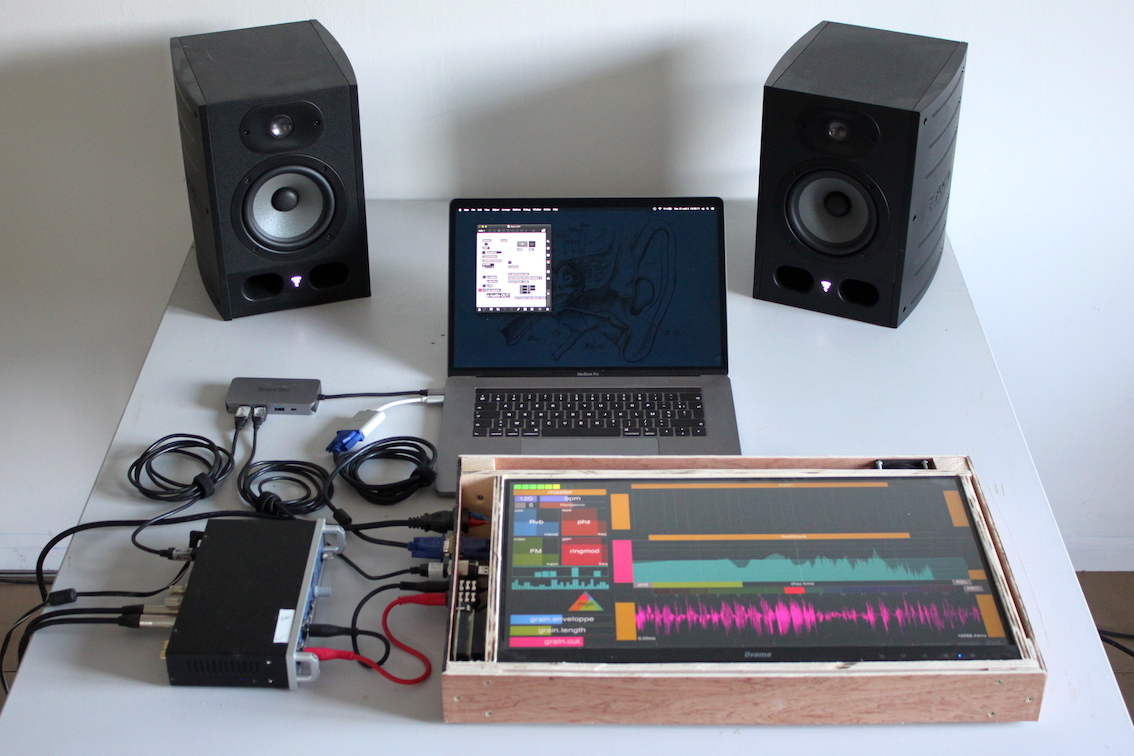
\includegraphics[width=\linewidth]{gfx/05_interfaces/Xypre_Overview_144dpi.jpg}
		\caption[Xypre: vue d'ensemble]{Xypre, vue d'ensemble du dispositif: Xypre, ordinateur avec Max, carte son, haut-parleurs}
		\label{fig:interface:xypre_unplugged}
	\end{minipage}
\end{figure}
%------------ Figure : filigramophone et xypre piezo -----------

%--------------------------------------------------------------
\section{Différentes faces de l'interface}

\subsection{Interface gestuelle ou interface sensible?}


\noindent Il est souvent question ``d'interface gestuelle'', voire de ``contrôleur gestuel'', lorsqu'on évoque les \glspl{IHM} utilisées pour l'interaction musicale. Comme nous l'avons vu au chapitre précédant, le geste y occupe une part importante, mais les interfaces de jeu ne 
%captent pourtant pas directement le geste, seulement ses éventuels effets sur différents types de capteurs. Ces capteurs peuvent impliquer un contact physique, tels les \gls{FSR} ou les potentiomètres qui constituent les capteurs les plus fréquemment utilisés sur les interfaces. Ces capteurs sont sensibles à des variations physiques telles que 
se limitent pas nécessairement à la captation du geste\footnote{Il serait plus exact de dire qu'elle ne captent pas les gestes, mais les effets des geste sur les capteurs.} : elle peuvent être sensibles au son\footnote{L'utilisation de microphones est courante et sera développée en particulier dans la section \ref{sec:interfaces:part_acoustique}}, à la température, la lumière\footnote{Voir par exemple les œuvres \textit{Light Thing} de Leaf Cutter John (\url{https://youtu.be/2jIlLHfSEfs}), ou encore \textit{Light Music} de Thierry de Mey}, la couleur, la géolocalisation\footnote{Voir en particulier les travaux d'Atau Tanaka \cite{tanaka_mobile_2004}, ou les instruments de Yann Seznec \url{https://www.impracticaldevices.com}}, aux signaux biologiques internes du corps\footnote{Voir notamment les travaux de Marco Donnarumma \cite{donnarumma_biophysical_2017}} et réagir de manière générale à différentes conditions environnementales.\\
\indent Par ailleurs, le geste possède un certain nombre de qualités qui ne sont pas forcément captées par l'interface, alors qu'elle sont effectivement perçues par le musicien et par le public et contribuent ainsi à la performance.\\
\indent Enfin, le ``geste'' qui vient contrôler les processus sonores dans les \glspl{DMI} peut être de nature virtuelle, prendre la forme de motifs pré-enregistrés qui peuvent être issus de toute sorte de source de données interprétées en tant que flux temporels, comme c'est le cas dans la ``sonification de données''\footnote{La sonification de données consiste à transformer des données non sonore, par exemple le cours de la bourse, en signaux audio. Cette technique est notamment utilisée, en dehors du champ musical, pour rendre perceptible des phénomènes ignorés, en s'appuyant en particulier sur nos capacités auditive à identifier des périodicités ou des intervalles de valeurs.} ou l'utilisation de ``modèles intermédiaires''\footnote{La notion de ``modèle intermédiaire'' sera décrit plus en détail dans le chapitre \ref{ch:algorithms}.}.\\
\indent Pour toutes ces raisons, il semblerait ainsi préférable de parler d'\textit{interface sensible}, plutôt que d'\textit{interface gestuelle} pour décrire les dispositifs d'interaction numériques pour la musique, leur caractéristique commune étant l'usage de capteurs (\textit{sensors}).
\indent Inversement, les haut-parleurs, les projections graphiques, les moteurs et actionneurs contrôlés algorithmiquement sont également \textit{à l'interface}, en ``sortie'' cette fois, entre le virtuel et le réel. Si de même, on considère plus souvent la partie ``captation'' que la partie ``diffusion'' lorsqu'on évoque les interfaces de jeu des \glspl{DMI}, il faut garder en vue que ces deux aspects s'entremêlent, non seulement dans la boucle de rétro-action qui se créé entre le musicien et l'instrument, mais également dans l'agencement concret des éléments matériels qui constituent le dispositif instrumental dans son ensemble, comme nous le verront dans ce chapitre.\\
\indent L'interface de jeu, en étant à la fois sensible à son environnement tout en rendant perceptible les artefacts générés par les algorithmes, traduit dans le réel la potentialité virtuelle d'un \gls{DMI}.


%%%%%%%%%%%%%%%%%%%%%%%%%%%%%%%%%%%%%%%%%
\subsection{Un support pour \textit{musiquer}?}

\noindent Les \glspl{DMI} sont des objets techniques dont l'interface est le support de diverses activités musicales: composition, interprétation, improvisation, pédagogie... En tant qu'agencements éphémères en perpétuelle évolution, leur interface est parfois le support de l'activité même de lutherie qui sert à les concevoir\footnote{L'exemple le plus manifeste de cette amalgame entre les fonctions d'instrument de performance, de composition et de lutherie est sans doute le \textit{live-coding}, dans lequel le clavier alphanumérique (ainsi que l'écran et les haut-parleurs) joue le rôle d'interface de jeu polyvalente pour ces différents contexte.}.

\todo{raccorder la suite avec ce début, e.g. virer ce paragraphe ?}
\noindent Les \glspl{DMI} intègrent souvent des matériaux sonores pré-composés, que le musicien peut déclencher et qui pourront tourner de manière autonome (paysages sonores, processus génératifs, drônes, etc.) et une part créée plus directement, qu'elle soit synthèse ou transformation de matériaux.\\
%\indent Les différents accès de l'interface de jeu doivent ainsi permettrent d'articuler ces différents pôles, en permettant la gestion du temps à différentes échelles. En particulier, les écrans \textit{multitouch}, s'ils permettent de gérer aisément de multiples processus lents (qu'on pourra visualiser et ajuster à l'écran), ne permettent guère une réactivité ``percussive'', telle que le permet un pad \gls{MIDI} ou un capteur échantillonné à fréquence audio.\\
\indent La granularité du contrôle joue également un rôle important dans cette perspective. Entre une note \gls{MIDI} qui ne déclenche qu'un événement ponctuel, un contrôleur continu qui envoie des données chaque fois qu'il est modifié et un capteur échantillonné à fréquence audio qui envoit ses valeurs 44100 fois par seconde, les possibilités de contrôle seront différentes en terme de réactivité et de finesse de modulation. Il faut donc prévoir les capteurs adéquats pour les processus que l'on souhaite contrôler en aval. Comme le faisait remarquer Max Mathews: \iquote{Il faut penser aux systèmes dans leur globalité pour obtenir quelque chose d'utilisable musicalement - on ne peut pas vraiment développer un capteur sans le mettre en perspective des programmes avec lesquels on va l'utiliser}\footnote{``One has to think of overall systems to get a musically useful thing — you can't really develop a sensor without relating it to the programs that you're going to use it with.'', Max Mathews, cité par Joel Chadabe dans \cite{chadabe_electric_1996}, p. 230}.\\
\indent Ceci n'est pas sans poser problème dans la perspective de modularité d'un \gls{DMI} que l'on aimerait pouvoir faire évoluer et adapter à différents contextes, différents projets. Une direction consiste à disposer d'une palette de capteurs différents afin de les agencer selon une ergonomie adaptée aux gestes qu'ils invitent, et d'adapter le logiciel, plus souple, à cette configuration\footnote{C'est par exemple la direction prise dans le Méta-Instrument de Serge de Laubier, qui peut charger tout une série d'instruments logiciels différents (cf. \cite{couprie_meta-instrument:_2018})}. Une autre direction, sans compromission de l'interface, consiste à accepter le fait qu'un instrument ne puisse pas tout faire et à prendre l'objet tel quel, dans sa complexité, avec ses résistances, avec ses choix esthétiques, avec son usage unique et singulier\footnote{C'est par exemple davantage le cas dans \textit{The Sponge} de Martin Marier (figure \ref{fig:interface:TheSponge}).}. 

\subsection{Instruments acoustico-électronico-numériques}

\noindent Si on les considère sur le plan matériel, il faut encore noter que les \glspl{DMI}, s'ils se caractérisent par l'usage de la computation numérique, sont aussi nécessairement des instruments électroniques, électriques et acoustiques. Il portent par conséquent l'héritage et les contraintes propres à ces différentes dimensions.\\
\indent Dans le domaine virtuel du code informatique, ces dimensions sont (trop\footnote{Cf. commentaires en section \ref{ch:algorithms:digital-material}}) bien séparées : la mécanique et l'électricité y sont absentes, et les signaux acoustiques et de contrôle bien rangés dans des variables indépendantes qui n'interagissent que si on le leur demande explicitement. Dans le monde réel, au contraire, l'interférence est la règle --~pour le meilleur et pour le pire~-- et il devient nécessaire d'isoler les différents signaux si l'on ne veut pas avoir à gérer la complexité de leur interaction : mettre les haut-parleurs loin des microphones, isoler les câbles électriques pour ne pas capter la radio, rajouter des mousses pour ne pas entendre les bruits mécaniques d'une frappe sur un capteur, etc. En se situant à la frontière, l'interface de jeu doit communiquer avec le virtuel mais aussi composer avec le réel.

%-------------------------------------------------------------

\subsection{Facteurs de formes: héritages et transpositions}
\label{sec:interfaces:heritages}

\noindent En partie libérés\footnote{En partie seulement, cf. § \ref{sec:interfaces:part_acoustique}} des contraintes de facteur de forme liées à l'acoustique, l'interface de jeu présentent un agencement et une topologie liés à des questions d'ergonomie d'une part mais aussi de divers héritages musicaux et extra-musicaux. Il ne s'agit pas ici de [les comparer avec pour but de] juger des directions les plus adaptées à la performance instrumentale, mais de constater leur usage effectif dans ce domaine par les musiciens numériques, en analysant leur intérêt respectif.

\subsubsection{Héritage instrumental}
\label{sec:interfaces:heritages:instrument}
%------------ Figure : Hyvibe et SmartMandolin -----------
\begin{figure}[!htbp]
	\captionsetup{format=plain}%
	\centering
	\begin{minipage}[t]{0.48\textwidth}
		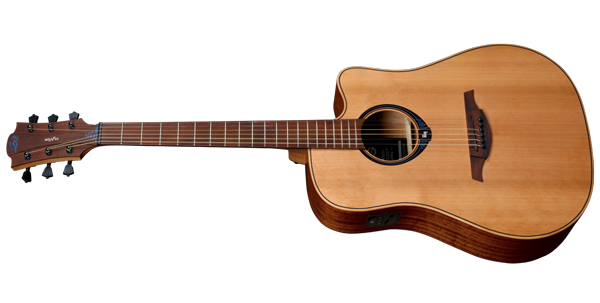
\includegraphics[width=\linewidth]{gfx/05_interfaces/HyVibe-guitar.png}
		\caption[La Smart Guitar de HyVibe]{La Smart Guitar de HyVibe ressemble à s'y méprendre à une guitare. Photographie © HyVibe}
		\label{fig:interface:hyvibe}
	\end{minipage}
	\hspace{.02\linewidth}
	\begin{minipage}[t]{0.48\textwidth}
	    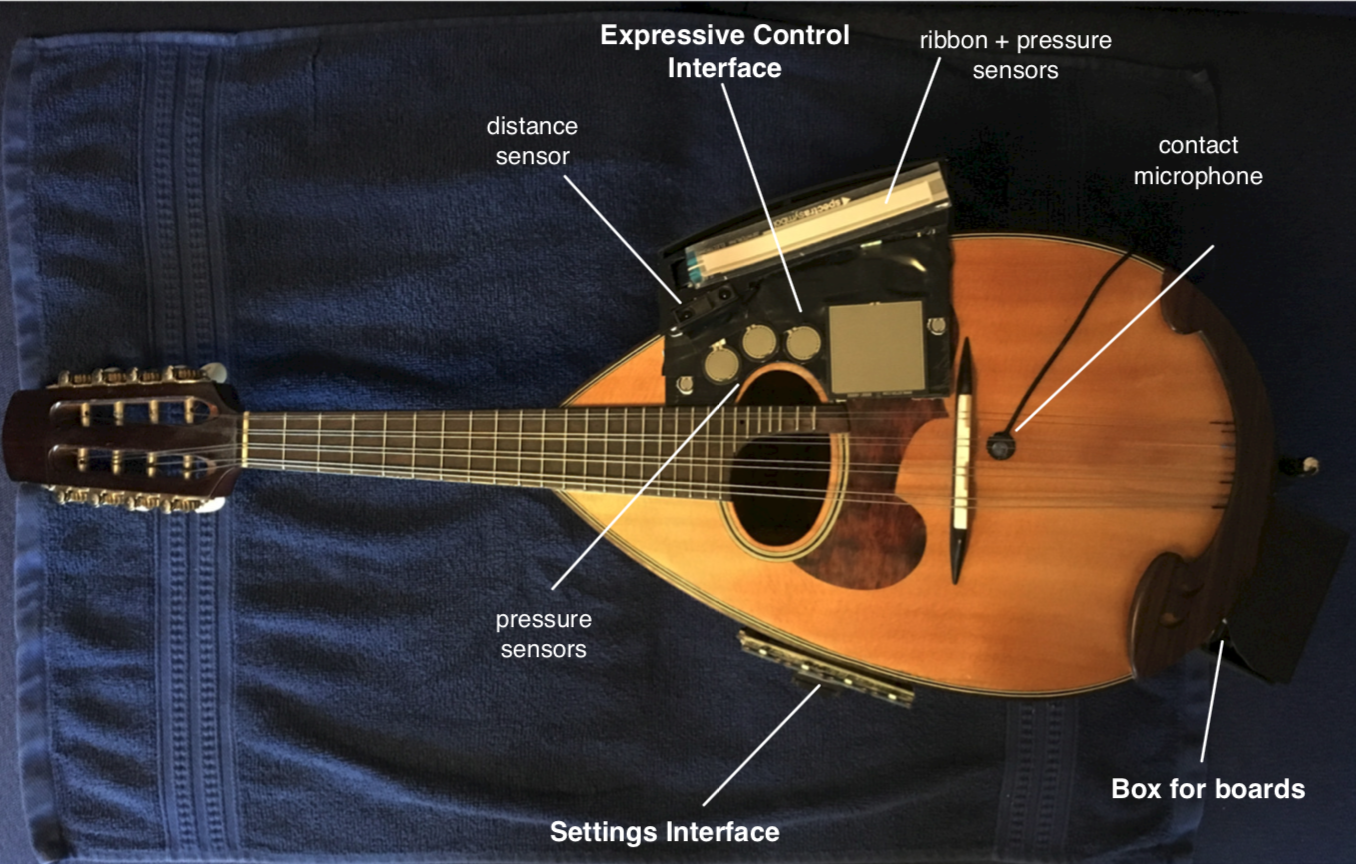
\includegraphics[width=\linewidth]{gfx/05_interfaces/Turchet-SmartMandolin.png}
		\caption[La Smart Mandolin de Lucas Turchet]{La Smart Mandolin de Lucas Turchet, avec capteurs ajouté sur la caisse. Photographie © Lucas Turchet}
		\label{fig:interface:smart-mandolin}
	\end{minipage}
\end{figure}
%------------ Figure : Hyvibe et SmartMandolin -----------
 \noindent L'héritage le plus évident est celui des techniques de jeu et du répertoire, qui prend une importance considérable dans le design des \glspl{DMI} inspirés d'instruments pré-existants, en particulier les instruments dits augmentés (cf. figure \ref{fig:interface:hyvibe} et \ref{fig:interface:smart-mandolin} et annexes \ref{appendix:turchet} et \ref{appendix:mamou-mani}). Cet héritage est le plus manifeste dans les instruments qui se destinent à une diffusion commerciale, en permettant un effet dilligence\footnote{notion définie par le médiologue Jacques Perriault, décrivant les protocoles mis en place pour l'adaptation d'une innovation en vue de son acceptation sociale (``Les premiers wagons avaient la forme des diligences.'')} entre instruments classiques et instruments nouveaux\footnote{\label{fn-Pinch}Cf. sur ce sujet l'analyse de Trevor Pinch dans \cite{pinch_why_2001} sur la présence de clavier sur les premiers synthétiseurs}.\\
 \indent Outre l'héritage gestuel liés aux modes de jeu sur les instruments acoustiques, les théories de la musique s'inscrivent de manière plus générale dans l'interface de jeu, en imprimant sur elles une topologie polarisée par les valeurs auxquelle elle recourt\footnote{Cf. section \ref{ch:visual_representation:music-theory}} (rythmes, intensités, hauteurs, timbre, etc.).


\subsubsection{Héritage scientifico-industriel}
\vspace{1em}
%------------ Figure : Sponge et Lungta ----------- 
% todo : utiliser subfig pour une légence commune ici ?
\begin{figure}[!htbp]
	\captionsetup{format=plain}%
	\centering
	\begin{minipage}[t]{0.48\textwidth}
		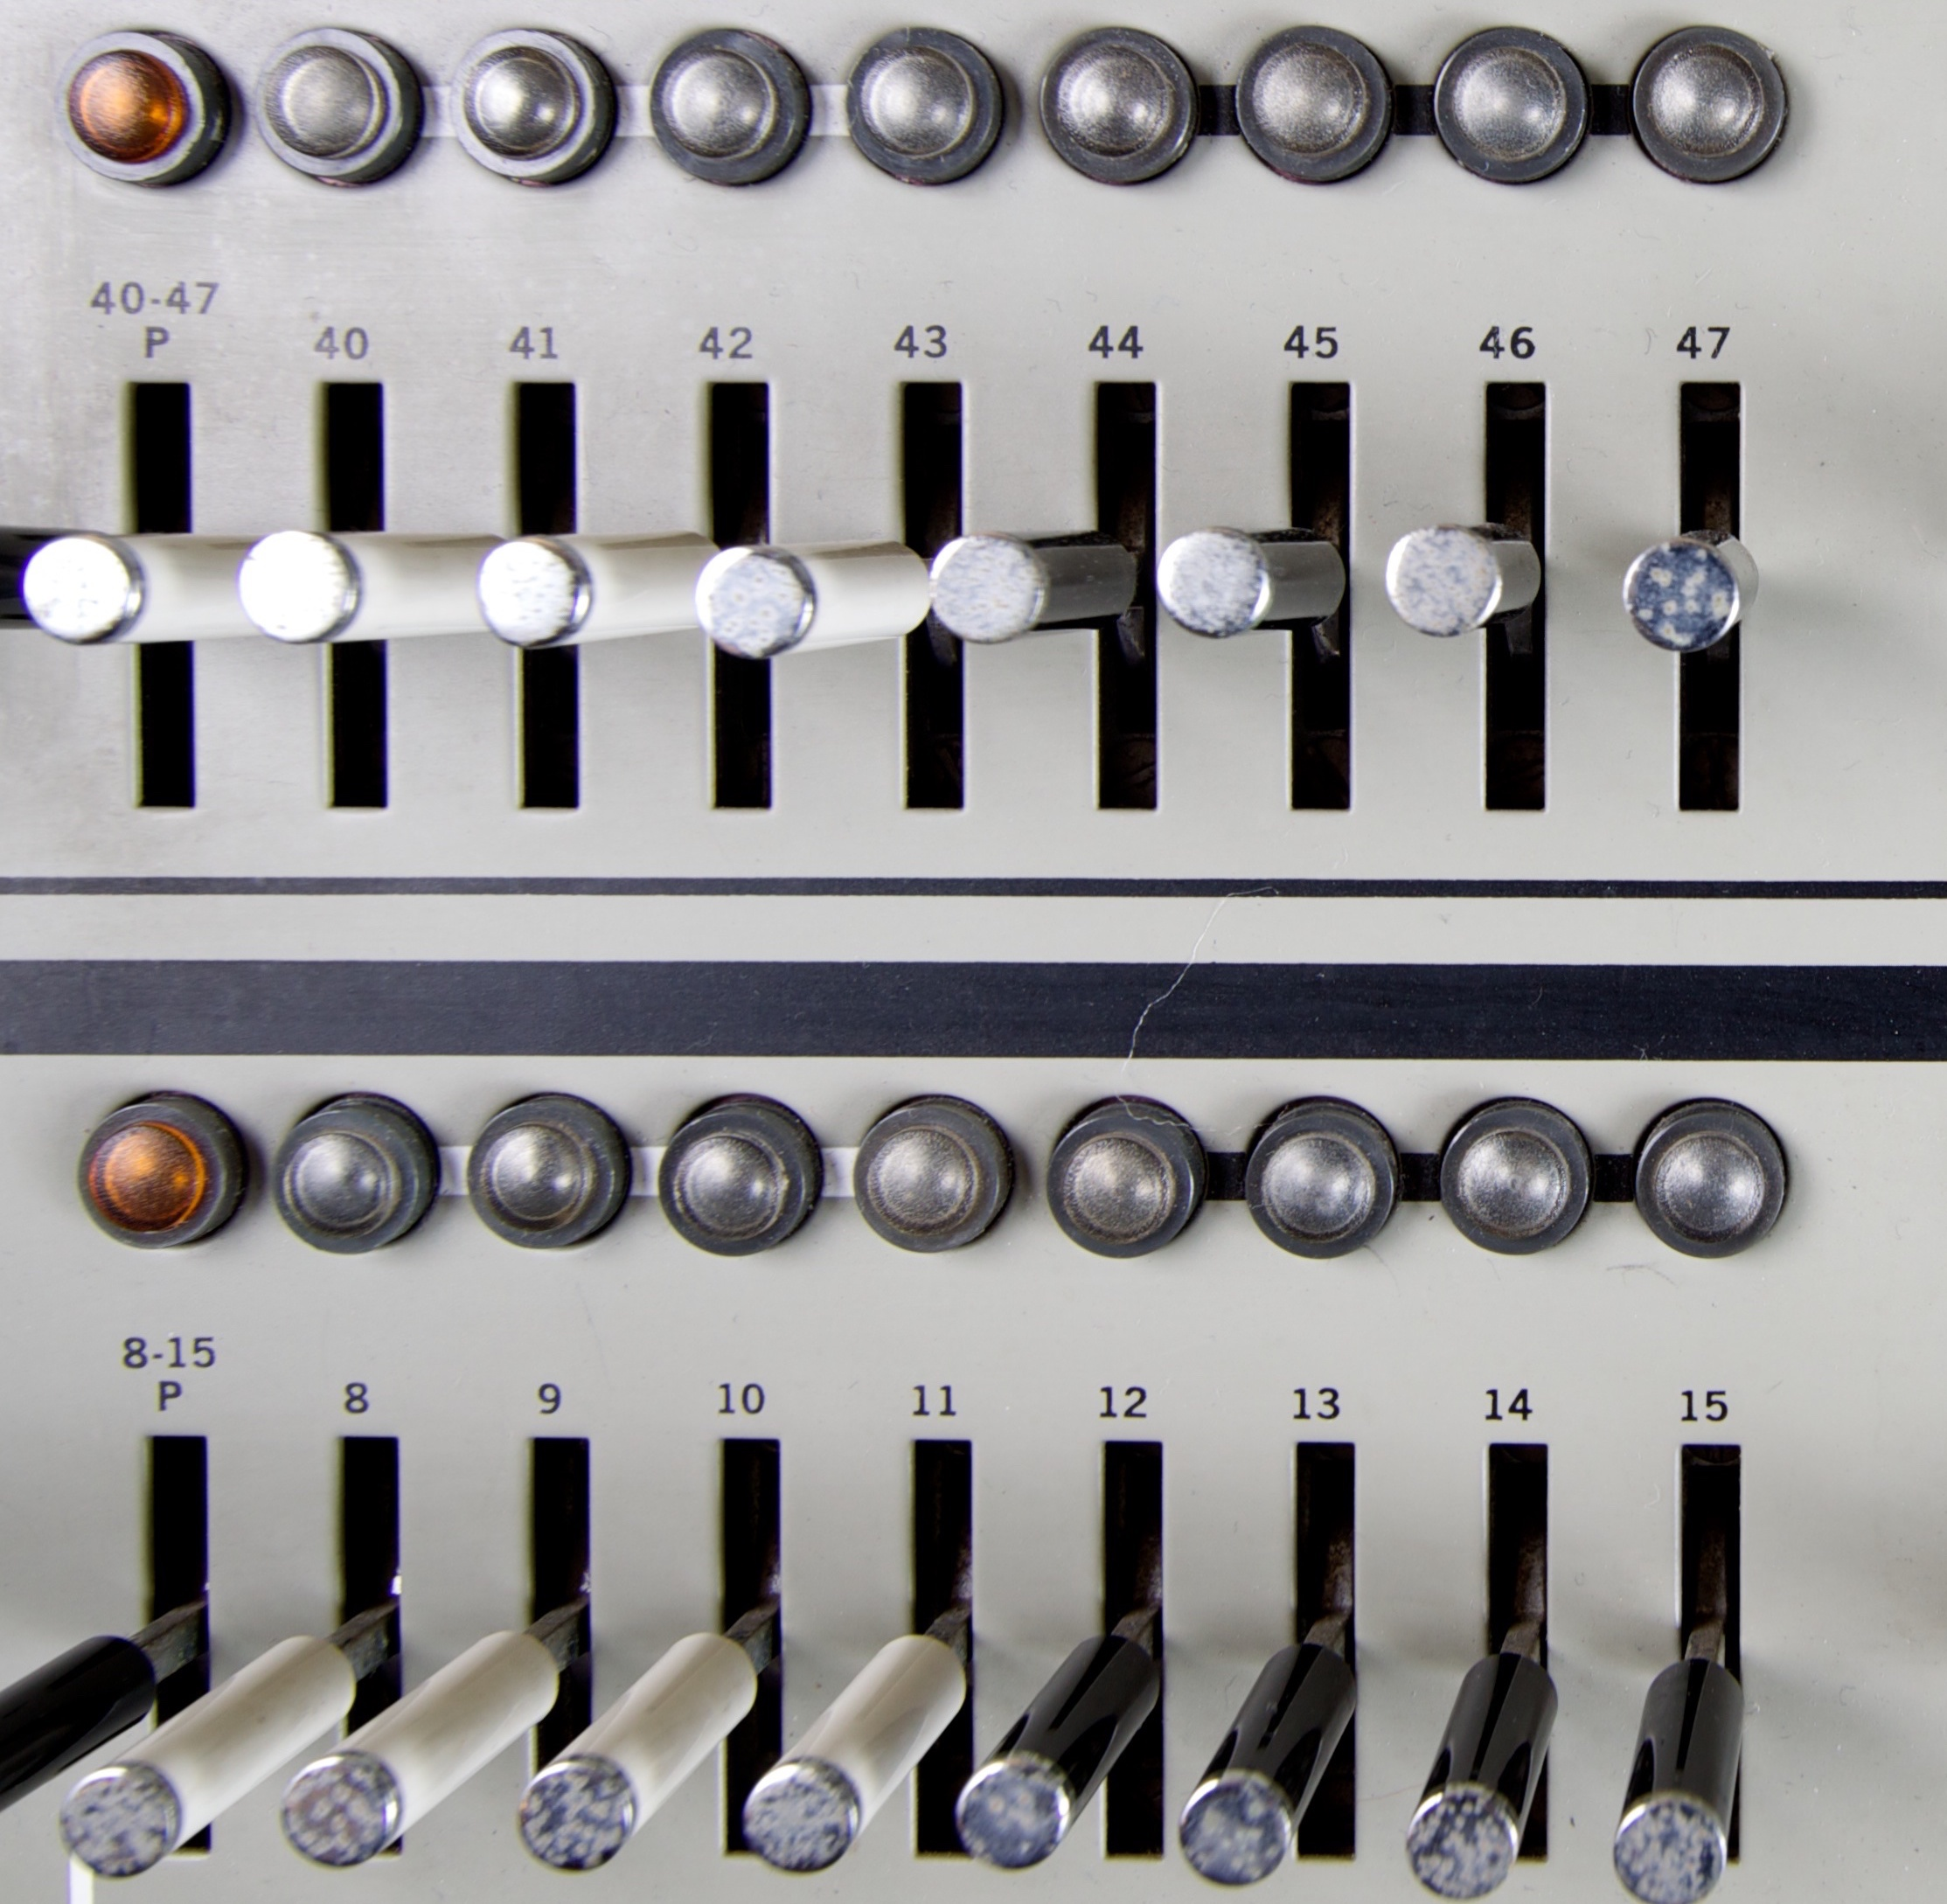
\includegraphics[width=\linewidth]{gfx/05_interfaces/IBM_System_360_Panel.jpg}
		\caption[L'interface du système 360 d'IBM]{Interface du\textit{ Système 360} d'IBM (détail), un ordinateur utilisé dans le domaine scientifique et l'ingénierie, commercialisé en 1965.}
		\label{fig:interface:ibm360}
	\end{minipage}
	\hspace{.02\linewidth}
	\begin{minipage}[t]{0.48\textwidth}
	    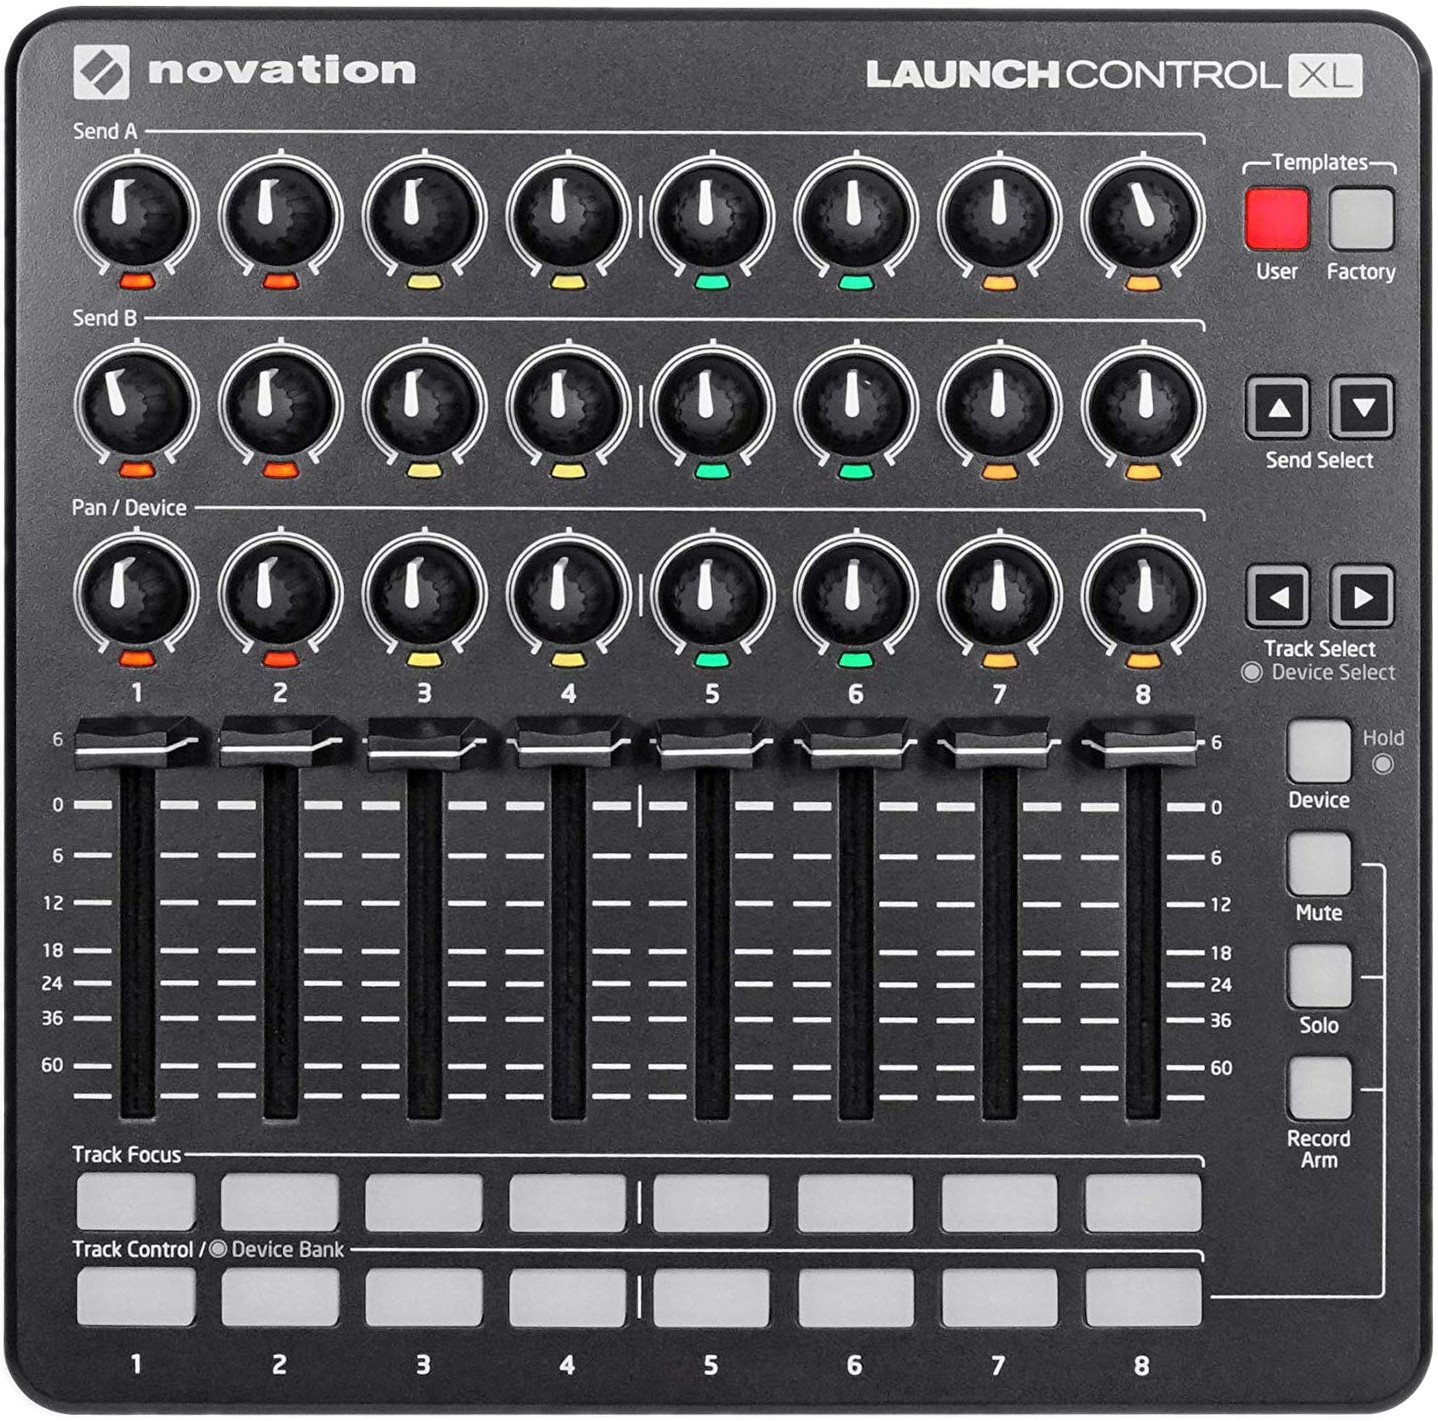
\includegraphics[width=\linewidth]{gfx/05_interfaces/NovationLaunchControlXL.jpg}
		\caption[L'interface MIDI Novation Launch-Control-XL]{Le \textit{Launch-Control XL} de Novation, une interface \gls{MIDI} dédiée à l'expression musicale, commercialisée en 2014.}
		\label{fig:interface:launchpad-controlXL}
	\end{minipage}
\end{figure}

\noindent L'informatique et l'ingénierie électronique, avec leur ancrage historique dans le domaine scientifique, industriel et militaire contribuent également à façonner les interfaces qui héritent des panneaux de commandes garnis de potentiomètres rotatifs, de faders et de LEDs clignotantes disposés en matrices rectilignes (cf. figure \ref{fig:interface:ibm360} et \ref{fig:interface:launchpad-controlXL}). Les interfaces graphiques connaissent le même genre d'influence avec l'héritage de la bureautique (dossiers et fichiers, poubelle, menus déroulants, etc.), omniprésent dans le design des logiciels et parfois imposé\footnote{Par exemple, le non-respect des règles de design édictées par Apple peut entraîner le refus de la publier (même gratuitement) sur l'app store.}. L'intérêt de ces interfaces est de présenter le maximum de contrôleurs indépendants, en facilitant le monitoring par une représentation uniforme adapté à une lecture rapide de leurs valeurs.

\subsubsection{Héritage du corps}

\noindent L'ergonomie, pensée en dehors de l'organologie classique, nous amène à considérer directement le corps, et plus particulièrement les mains. Comme l'explique Serge de Laubier (cf. Annexe \ref{appendix:delaubier}) :\\
\iquote{(...) quand on fabrique un instrument il y a une contrainte, c'est le corps et donc forcément, il faut que les instruments, en tout cas ceux qui fonctionnent bien, soient quand même relativement bien adaptés au corps (...) et la première contrainte c'est celle des mains (...) parce que c'est [le membre] le plus agile, je pense, le plus agile, rapide, réactif.} Un certain nombre d'instruments comme ``The Hands'' de Michel Waisvisz --~dont le nom parle de lui-même~-- ou le Méta-Instrument de Serge De Laubier sont ainsi directement conçus à partir de l'ergonomie de la main.\\
\indent Le corps entier peut être utilisé de manière instrumentale, en particulier dans la domaine chorégraphique. Si les interactions entre la danse et les systèmes électroniques interactifs ont plus de 50 ans\footnote{En 1965, Merce Cunningham, John Cage et David Tudor utilisaient déjà des capteurs photo-électriques pour contrôler les processus musicaux dans la performance \textit{Variation V}.}, les interfaces de \textit{motion capture}, devenues plus accessibles depuis le début du \siecle{21}~siècle\footnote{On pense ici aux webcams et aux nouveaux usages permis par les progrès de l'analyse d'image et d'apprentissage, à la Kinect de Microsoft, au Leap-motion, aux capteurs de type \gls{AHRS}, etc.} ont multiplié le nombre de performances chorégraphiques dans lesquelles l'expertise du mouvement corporel est directement utilisée pour le contrôle de processus musicaux\footnote{Voir notamment les créations de Myriam Gourfink et Kasper Toeplitz, et les travaux de Frédéric Bevilacqua, e.g. \cite{bevilacqua_gesture_2011}}.\\
\indent Enfin, les mouvements internes du corps tels que la tension musculaire, les battements du cœur, ou l'activité cérébrale sont envisageables pour l'interaction instrumentale en utilisant des capteurs de signaux bio-physiques (ECG, EEG, EMG, etc.). Une analyse détaillée de cette perspective est proposée par Atau Tanaka et Marco Donnarumma dans \cite{tanaka_body_2019}, qui sont eux-mêmes les auteurs de plusieurs projets et performances musicales dans cette veine.

\subsubsection{Héritage poétique de l'objet}

\noindent C'est parfois l'absence d'héritage instrumental qui est recherchée. Martin Marier\footnote{Voir les vidéos sur \url{http://www.martinmarier.com}} explique ainsi le design de l'interface ``The Sponge'' \cite{marier_sponge_2010} (figure \ref{fig:interface:TheSponge}), dont il souhaite qu'elle ne fasse référence à aucun instrument existant, afin que son apparence ne dicte pas de paradigme musical, ni ne créé d'attente particulière du public en terme de composition.\\
%------------ Figure : Sponge et Lungta -----------
\begin{figure}[!htbp]
	\captionsetup{format=plain}%
	\centering
	\begin{minipage}[t]{0.48\textwidth}
		\includegraphics[width=\linewidth]{gfx/05_interfaces/epongeCloseUp_prestonBeebe.jpg}
		\caption[``The Sponge'' de Martin Marier]{``The Sponge'', une interface instrumentale de Martin Marier. Photographie © Preston Beebe.}
		\label{fig:interface:TheSponge}
	\end{minipage}
	\hspace{.02\linewidth}
	\begin{minipage}[t]{0.48\textwidth}
	    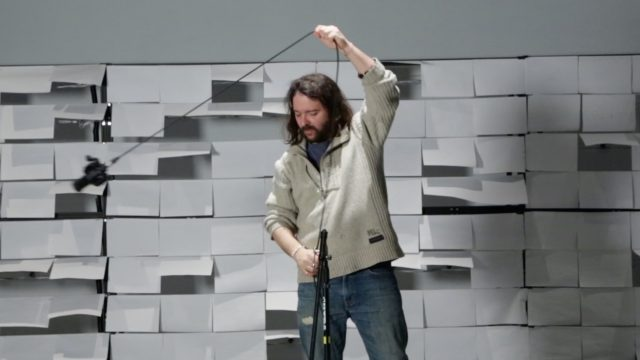
\includegraphics[width=\linewidth]{gfx/05_interfaces/Saint-Denis-Lungta.jpg}
		\caption[LUNGTA de Patrick Saint-Denis]{LUNGTA, une installation performative basée sur une matrice de feuilles de papier controlée algorithmiquement. Photographie © Patrick Saint-Denis.}
		\label{fig:interface:lungta}
	\end{minipage}
\end{figure}
%------------ Figure : Sponge et Lungta -----------
\indent L'instrument est également un objet mis en scène et son rôle scénographique vient parfois façonner son instrumentalité. C'est le cas par exemple dans les créations de Patrick Saint-Denis\footnote{Voir les vidéos sur \url{http://www.patricksaintdenis.com}}, qui \iquote{part de l'objet} et \iquote{poursuit l'idée des objets animés par le son} (cf. figure \ref{fig:interface:lungta} et annexe \ref{appendix:saint-denis}).\\
\noindent L'idée d'utiliser la connotation des objets employés comme instruments de musique était également centrale dans la performance audiovisuelle \textit{Donjon}\footnote{Plus de détails sur \url{http://vincentgoudard.com/donjon/}} (Cécile Babiole, Jean-Michel Dumas, Vincent Goudard), dans laquelle des bornes d'arcades des années 1980 reconverties, à l'aide d'une électronique \textit{ad hoc}, en interfaces de jeu pour le contrôle de l'image et du son en temps réel, faisaient écho à l'esthétique musicale et visuelle de la performance (figure \ref{fig:interface:donjon}).\\
%------------ Figure : Donjon -----------
% \begin{figure}[!htbp]
% 	\captionsetup{format=plain}%
% 	\makebox[\linewidth][c]{%
% 		\begin{subfigure}[b]{.5\textwidth}
% 			\centering
% 			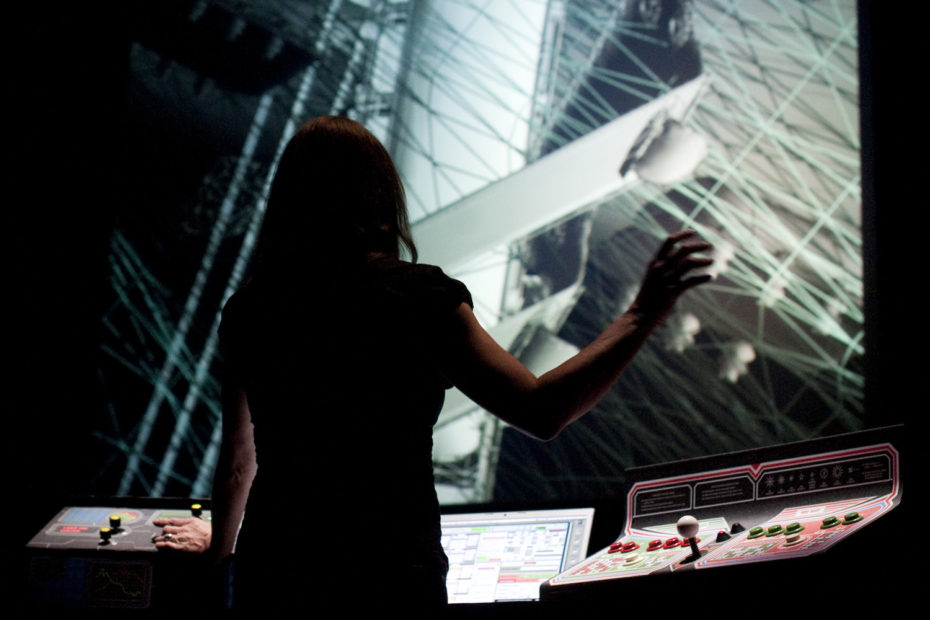
\includegraphics[width=\linewidth]{gfx/05_interfaces/Donjon_Cecile.jpg}
% 			%\caption{Son vers gestes}
% 		\end{subfigure}%
% 		\hspace{.01\linewidth}
% 		\begin{subfigure}[b]{.5\textwidth}
% 			\centering
% 			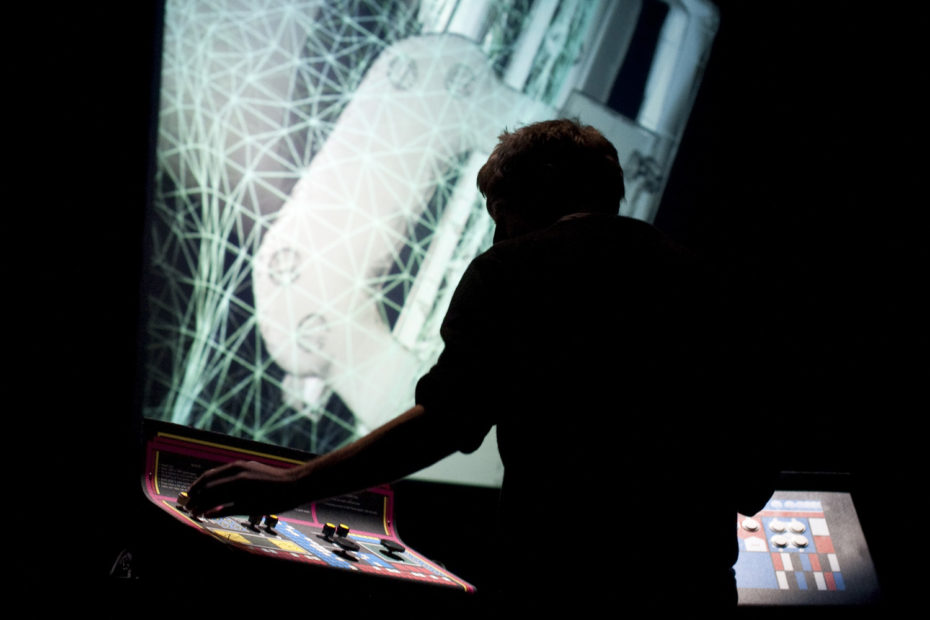
\includegraphics[width=\linewidth]{gfx/05_interfaces/Donjon_Vincent.jpg}
% 			%\caption{Instrument vers gestes}
% 		\end{subfigure}%
% 	}
% 	\caption[Donjon, performance audiovisuelle utilisant des bornes d'arcade]{Des bornes d'arcade, à l'esthétique très connotée années 1980, utilisées comme interface de jeu dans la performance audiovisuelle \textit{Donjon}. A gauche: Cécile Babiole, à droite: Vincent Goudard. Photographie: Sébastien Bozon}
% 	\label{fig:interface:donjon}
% \end{figure}
%------------ Figure : Donjon -----------
%------------ Figure : Donjon -----------
\begin{figure}[!htbp]
	\captionsetup{format=plain}%
	\makebox[\linewidth][c]{%
		\begin{subfigure}[b]{.5\textwidth}
			\centering
			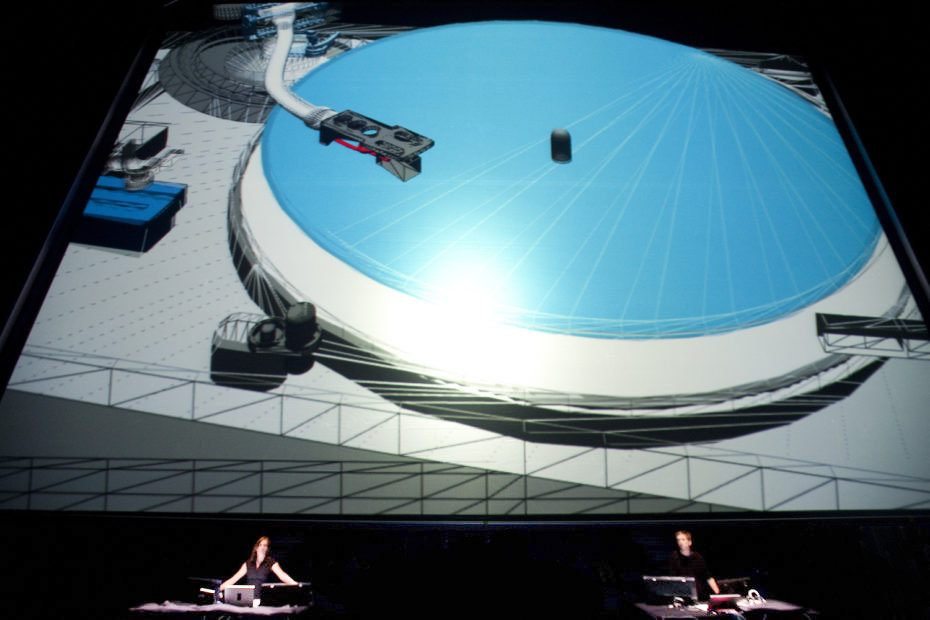
\includegraphics[width=\linewidth]{gfx/05_interfaces/Donjon_Filature2.jpg}
			%\caption{Son vers gestes}
		\end{subfigure}%
		\hspace{.01\linewidth}
		\begin{subfigure}[b]{.5\textwidth}
			\centering
			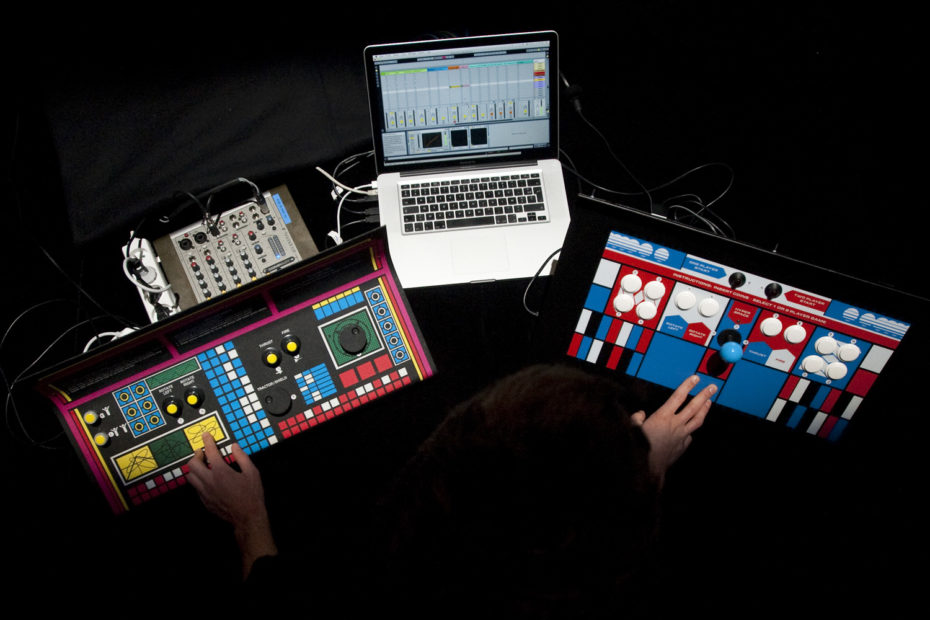
\includegraphics[width=\linewidth]{gfx/05_interfaces/Donjon_Vincent_interfaces.jpg}
			%\caption{Instrument vers gestes}
		\end{subfigure}%
	}
	\caption[Donjon, performance audiovisuelle utilisant des bornes d'arcade]{Des bornes d'arcade, à l'esthétique très connotée, utilisées comme interface de jeu dans la performance audiovisuelle \textit{Donjon}. A gauche: Vue d'ensemble de la scène, à droite: détail des interfaces de Vincent Goudard. Photographies: Sébastien Bozon.}
	\label{fig:interface:donjon}
\end{figure}
%------------ Figure : Donjon -----------
\indent L'interface est ainsi forgée par la force d'évocation poétique des objets, qui dépasse le strict cadre fonctionnel de la relation instrumentale. La mythologie qui leur est associée polarise le jeu du musicien et l'écoute du public, \iquote{comme s'il y avait un arrière plan imaginaire de tout ce que ça draine d'histoire, de projections} (cf. Annexe \ref{appendix:dumeaux}). On retrouve cette même fonction poétique dans ``l'Olitherpe'', instrument joué par Patricia Dallio\footnote{Site web : \url{http://www.patriciadallio.com}. Voir le documentaire ``L'Olitherpe et la teneur de l'air'' (\url{https://vimeo.com/224494409}) à propos des considérations faites ici.}, qui se présente comme un agencement de capteurs intégrés dans des objets de récupération. Les associations morphologiques et fantasmagoriques entre mouvements de l'instrumentiste, fonction des capteurs et forme des objets tient un rôle essentiel dans la construction de l'interface de jeu: par exemple, le capteur infra-rouge évocant des yeux est intégré dans un vieux phare de vélo.\\
\indent On peut voir dans la démarche artisanale et \gls{DIY} des lutheries numériques l`importance accordée à la charge affective de l'instrument; les interfaces numériques (tels que les contrôleurs \gls{MIDI}) vendues dans le commerce sont en effet souvent issus d'une production industrielle et faits de matériaux plastiques qui à l'inverse du bois d'un violon, ne porte pas la trace organique des fibres du bois ou celle du geste artisanal imprimé par le luthier et se retrouve, d'une certaine manière, dépourvu d'histoire.

%%%%%%%%%%%%%%%%%%%%%%%%%%

\section{Matériaux}
\label{sec:interfaces:materials}

%-------------------------- Figure : table du luthier numérique ----------------------------------
\begin{figure}[!htbp]
	\captionsetup{format=plain}%
	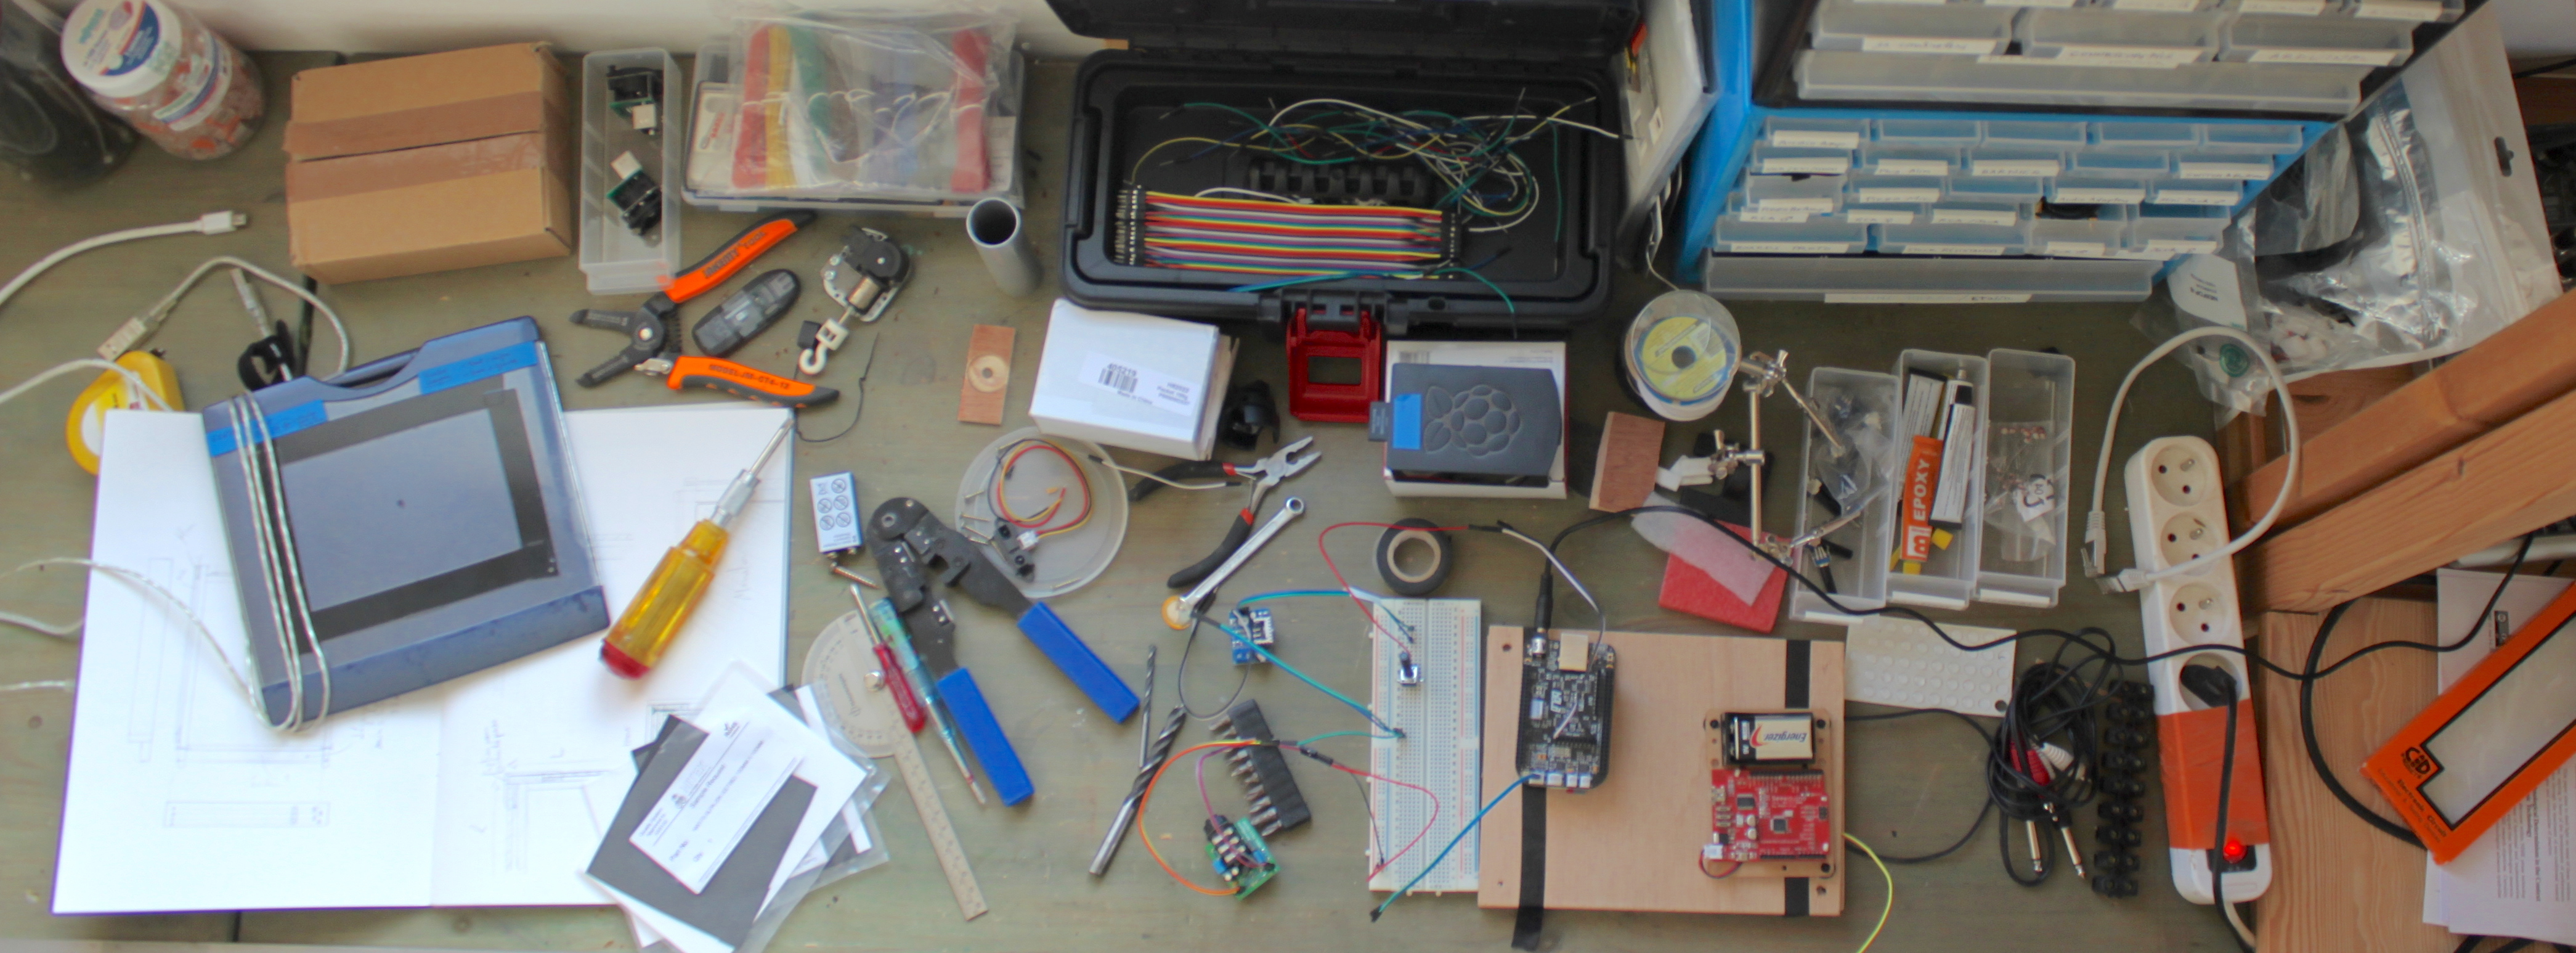
\includegraphics[width=\textwidth]{gfx/05_interfaces/lutherie-worktable.jpg}
	\caption[Matériaux sur la table d'un luthier numérique]{Matériaux sur la table d'un luthier numérique.}
	\label{fig:interface:table-luthier}
\end{figure}
%-------------------------- Figure : table du luthier numérique ----------------------------------

\noindent Une partie de la recherche sur les \gls{IHM} est motivée par la perspective d'une ``disparition de l'interface'' (\cite{weiser_computer_1991, dey_distributed_2001, hui_towards_2017}), au profit d'une \textit{informatique ubiquitaire} permettant une interaction directe avec les contenus plutôt qu'au moyen d'un support intermédiaire. Cette disparition de l'interface est liée --~parfois à tort, comme nous l'avons objecté dans le chapitre précédent~-- à l'idée de ``transparence'' de l'interaction, c'est à dire de correspondance entre l'attente d'un utilisateur et le résultat de son interaction avec la machine. Cette vision a été également appliqué au contexte de l'interaction musicale et, de façon relativement paradoxale, par des auteurs\footnote{On peut notamment citer Marc Leman :\iquote{What is needed is a transparent mediation technology that relates musical involvement directly to sound energy. Transparent technology should thereby give a feeling of non-mediation, a feeling that the mediation technology ``disappears'' when it is used. Such a technology would then act as a natural mediator for search-and-retrieval purposes as well as for interactive music-making.} \cite{leman_embodied_2008} ou encore Sydney Fels : \iquote{The more transparent the mapping is, the more expressive the device can be. The degree of mapping transparency for the player and audience form orthogonal axes of a graph into which devices can be placed. Full transparency for the player means that the device's output exactly matches the player's expectation and control.} \cite{fels_mapping_2002}.} fermement attachés à la notion d'\textit{embodiement}.\\
\indent Cependant, et paraphrasant la citation de Stravinsky en exergue de ce chapitre, les matériaux ne doivent pas être méprisés. Ils offrent de nombreuses possibilités, en terme de sensation, d'appui et de repos, et on peut s'en saisir aussi facilement que les délaisser--~quand il s'avère plus compliqué de délaisser un système immersif, voire ses propres pensées.\\
\indent Ce section regroupe une liste non-exhaustive de matériaux pouvant se retrouver sur la table de travail d'un luthier numérique. Ils sont regroupés en familles: matériaux bruts, capteurs, processeurs, mais l'agencement instrumental rend parfois leurs frontières poreuses (par exemple, un textile resistif et une plaque de métal peuvent servir à réaliser un capteur de pression). Cette liste dresse néanmoins un paysage général de ce répertoire, en en soulignant certains traits.

\subsection{Matériaux structurels}

\noindent Dans les instruments ``à contact'' (c'est-à-dire dans lesquel l'interaction passe par un rapport tactile avec l'interface de jeu), les matériaux structurels définissent l'agencement physique du \gls{DMI}: non seulement la distribution spatiale de son affordance mais également la cohésion et les liaisons mécaniques entre les différents capteurs. En effet, on touche rarement les capteurs de manière directe : ils sont recouverts, enveloppés, intégrés dans un objet matériel plus ou moins complexe, possédant son propre état de surface, son propre jeu mécanique, en liaison avec le reste du dispositif. Ils assurent la jonction autant que l'isolement des différent capteurs.
\vspace{-1em}
\begin{itemize}[noitemsep]
	\item \textbf{le bois}: Le contreplaqué est très souvent utilisé pour le prototypage rapide des \glspl{DMI} (cf. figure \ref{fig:interface:d-box}). Disponible en plaques de différentes épaisseurs, facilement découpable, perçable, collable et usinable par machine \gls{CNC}, il est un matériau très répandu dans la fabrication \gls{DIY} et les \glspl{makerspace}. Par ailleurs, le bois est historiquement le matériau phare de la lutherie acoustique. Il est par conséquent présent dans les instruments augmentés issus de lutheries acoustiques, mais son importance historique l'ancre de surcroît dans l'imaginaire collectif de l'instrument de musique. L'image d'Epinal de l'atelier du luthier est remplie de copeaux et de ciseaux à bois et, de même que les claviers, le bois contribue à donner un sentiment d'instrumentalité à un dispositif numérique. Ainsi, bien que n'ayant aucun rôle fonctionnel (excepté celui de sa sensualité), le bois massif est utilisé pour son caractère noble et évocateur sur certains instruments numériques high-tech, tels que le Linnstrument, le SoundPlane (cf. figure \ref{fig:interface:soundplane}).
	%------------------ Figure : D-Box and soundplane ---------------------
	% indenter avec https://tex.stackexchange.com/questions/54448/figure-with-caption-within-an-itemize-list-not-indenting-correctly ?
	\begin{figure}[!htbp]
		\makebox[\textwidth][c]{%
			\begin{subfigure}[b]{.4\textwidth}
				\centering
				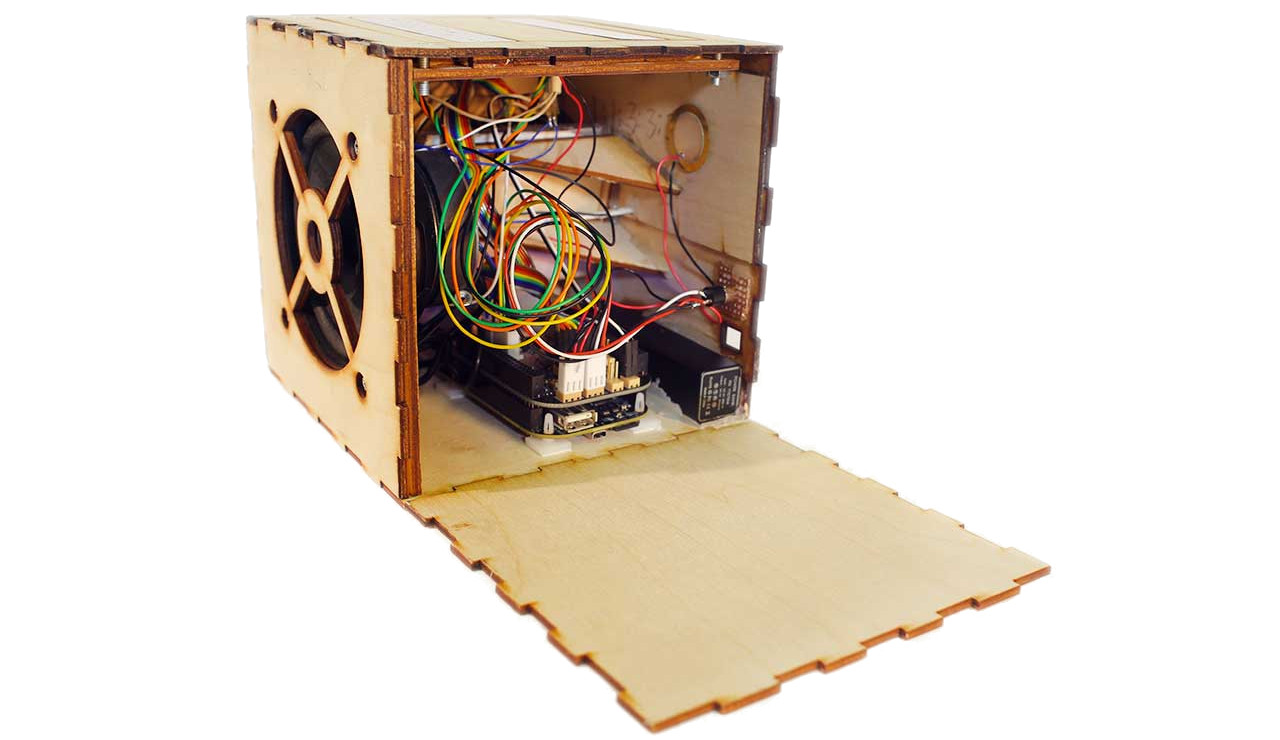
\includegraphics[width=\linewidth]{gfx/05_interfaces/d-box.jpg}
				\caption[La D-Box, un instrument ``hackable'']{La D-Box (cf. \cite{zappi_design_2014})}
			\label{fig:interface:d-box}
			\end{subfigure}%
			\begin{subfigure}[b]{.6\textwidth}
				\centering
		    	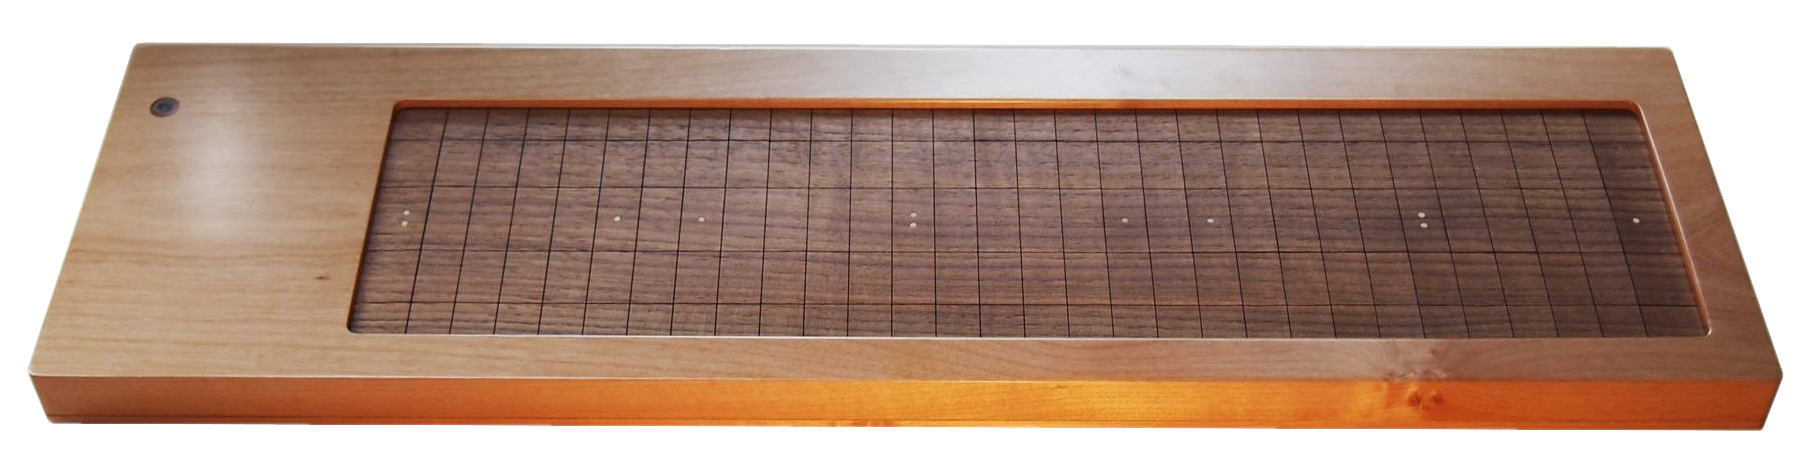
\includegraphics[width=\linewidth]{gfx/05_interfaces/soundplane.png}
				\caption[Le SoundPlane de Madrona Labs]{Le SoundPlane. © Madrona Labs}
				\label{fig:interface:soundplane}
			\end{subfigure}%
		}
		\caption{Contreplaqué ou massif : deux usages du bois dans les \glspl{DMI}.}
	\end{figure}
	%------------------ Figure : D-Box and soundplane ---------------------
	\item \textbf{le métal} est couramment utilisé pour les chassis et les coques de revêtement des machines électriques et électronique. En dehors de ses propriétés de résistance mécanique, sa conductivité permet d'isoler les composants de faux contacts et de perturbations électromagnétiques et notamment d'éviter le ``bruit de masse'' qui peut survenir quand un équippement électrique tel qu'un \gls{DMI} n'est pas relié à la masse. Le métal possède également des propriétés de résonance acoustique qui en font un matériau intéressant pour la captation et la diffusion électro-acoustique, et utilisé par exemple dans le diffuseur ``Gong'' de l'onde Martenot.
	\item \textbf{le plastique} offre de grande facilités de thermoformage, moulage, collage, perçage, gravage, qui permettent d'obtenir toute sorte de forme et notamment de s'adapter à l'ergonomie du corps (e.g. la main du MI). Les propriétés de transparence du \gls{PMMA}\footnote{aussi connue sous le nom commercial Plexiglass} permettent de l'utiliser au dessus d'un écran. L'essor des imprimantes 3D depuis le début du \siecle{21}~siècle a également contribué à son utilisation pour le prototypage rapide hors contexte industriel, dans les pratiques \gls{DIY} et les \glspl{makerspace}.
	\item \textbf{la mousse} est généralement utilisée pour ses propriété d'isolation phonique et vibratoire, mais également comme matériau tampon, pour augmenter la course des capteurs de pression (\gls{FSR}). Il existe de nombreuses sortes de mousses, offrant des nuances différentes d'enfoncement, de résiliance et affectant considérablement la sensation tactile sur ce type de capteurs.
	\item \textbf{le textile} a enfin été utilisé dans un certain nombre de \glspl{DMI} et de manière plus générale dans tout le champ d'interaction entre le domaine de la confection textile et de l'électronique, généralement désignée sous le terme de ``\textit{wearable electronics}''\footnote{Cf. la revue proposée dans \cite{stoppa_wearable_2014}}. La possibilité d'intégrer des fibres conductrices entrelacées dans le textile (``\textit{e-textile}'') a ainsi donné lieu à plusieurs développements de surfaces multitouch \cite{freed_application_2008, donneaud_designing_2017, wicaksono_fabrickeyboard:_2017} ou de vêtements munis de capteurs \cite{hayafuchi_musicglove_2008, serafin_controlling_2014, myllykoski_prototyping_2015}.
	\item \textbf{le verre} est utilisé en particulier pour le caractère cristallin de sa résonnance acoustique (e.g. Cristal Baschet, glass-harmonica). Une étude des cristallophones et de l'exploitation des qualités timbrales du verre dans les instruments électroniques a été proposée dans \cite{jensenius_evaluating_2010, frounberg_glass_2010}. Sa transparence permet d'offir un support tangible à un écran où une caméra (voir par exemple \cite{savary_dirti_2012} ou la section \ref{sec:interfaces:phylogenese:xypre}). Plus difficile à travailler, son usage est toutefois moins courant dans les lutheries en général.
\end{itemize}

\subsubsection{Systèmes ``intermédiaires'' physiques}

\noindent Outre l'aspect structurel ``statique'', de nombreaux systèmes mécaniques sont utilisés dans les \glspl{DMI}, venant modifier l'agencement spatial de l'instrument, ou transformer la relation avec les capteurs. Certains sont directement issus des lutheries traditionnelles; c'est le cas par exemple pour les touches de clavier, dont l'implémentation varie entre le simple contact direct sur un interrupteur bipolaire, et des systèmes plus complexes imitant la mécanique du clavier de piano (lestage des touches, mesure de la vitesse d'enfoncement, de pression et de relâchement la touche, etc...) (figure todo), d'autres sont d'origine extra-instrumentale, par exemple le système de pantographe développé par Ali Moméni pour contrôler un stylet de tablette graphique, présenté dans \cite{zbyszynski_ten_2007} ou le système d'articulation des bras sur le Méta-Instrument de Serge de Laubier). La notion de ``modèle intermédiaire'', transposée dans le domaine numérique, sera présentée plus en détail dans la section \ref{sec:algorithms:MID}.


%%%%%%%%%%%%%%%%%%%%%%%%%%%%%%%%%%%%%%%%%%%%%%%%%%%%%%%%%

\subsection{Feed-in: capteurs}

\noindent Une grande diversité de capteurs est disponible sur le marché, mesurant différentes grandeurs physiques : position, distance, pression, orientation, flux d'air, son, lumière, humidité, température, champ magnétique, présence, contact, etc. Pour chaque grandeur mesure, la donnée sera encore variable selon les caractéristiques du capteur : sensibilité, résolution, précision, linéarité, bande passante, temps de réponse, etc. À cette diversité s'ajoute encore le fait que les capteurs intègrent de plus en plus souvent des algorithmes de traitement de signal, parfois programmables. Ces capteurs dits ``intelligents'' peuvent notamment réaliser des opérations de filtrage, mais également de la fusion de données permettant de renvoyer des informations de plus haut niveau\footnote{C'est le cas par exemple sur les capteurs dits \gls{AHRS}, sur les interfaces multitouch qui analysent une matrice de capteurs pour en extraire la position des points de contact}. Enfin, comme nous l'avons dit précédemment, les capteurs sont rarement utilisés de manière brute mais s'intègrent dans un agencement à la fois matériel, mécanique, électronique et algorithmique qui affecte leur réponse du tout au tout.\\
\indent L'utilisation spécifique de cette diversité de capteurs dans le domaine des lutheries numériques a été l'objet de nombreuses études qualitatives et quantitatives, menées en particulier depuis ces deux dernières décennies par l'équipe de Marcello Wanderley à l'\gls{IDMIL}\footnote{Voir notamment : \cite{wanderley_choice_2000, hollinger_evaluation_2006, marshall_sensor_2009, vigliensoni_quantitative_2012, medeiros_comprehensive_2014} ainsi que le site \url{https://sensorwiki.org} qui rassemble un grand nombre d'informations techniques utiles sur les capteurs et les interfaces.}. En fournissant une analyse détaillée de leurs caractéristiques et en les intégrant dans des réalisations instrumentales fonctionnelles et jouées, ces études fournissent une base de données documentaire inestimable pour aider les luthiers numériques à ne pas se perdre dans cette multitude d'options possibles.\\
\indent Cependant, la généralisation de leur évaluation à des fins musicales reste délicate, en raison du fait que les instruments de musique constituent, comme nous l'avons déjà décrit dans les chapitres précédants, des \glspl{IHM} d'un genre particulier.

\subsubsection{Une analyse critique de la relation entre capteur et fonction musicale}

\noindent Un certain nombre d'études ont par ailleurs proposé une analyse de l'adéquation entre capteurs et fonctions musicale (e.g. \cite{vertegaal_towards_1996, goudeseune_interpolated_2002}), en mettant les aspects statique, dynamique, absolu ou relatif des valeurs transmises par les capteurs en regard de ces mêmes aspects appliqués à des valeurs musicales (en particulier la hauteur), dans l'optique d'évaluer qualitativement l'adéquation entre le choix des capteurs et le type de contrôle musical\footnote{Cette perspective reflète de manière plus générale une tendance de l'époque à vouloir répliquer le modèle instrumental classique ou la relation entre le geste et le résultat sonore est très directe. La remarque en conclusion de l'article d'Ungvary et Vertegaal \iquote{(...) a good causal mapping can ensure that tension is properly translated to the audible result.} en est révélatrice. Voir également la position de Claude Cadoz en ce sens au chapitre \ref{ch:gesture}.}. Bien qu'instructives et utiles dans la perspective d'une relation de mimétisme\footnote{Et les relations de mimétisme jouent un rôle essentiel dans les lutheries numériques, comme l'analyse Thor Magnusson dans \cite{magnusson_ergomimesis_2018}} univoque entre le mouvement gestuel et le mouvement d'un paramètre sonore, ces études mettent cependant de côté un aspect essentiel des \glspl{DMI}, à savoir la possibilité sans pareil des ordinateurs à traiter le signal et changer son échelle, transformer le continu en discret, l'absolu en relatif, l'instantané en différé, le statique en dynamique, et inversement, et plus encore.\\
%-------------------------- Figure : Vertegaal-transducer-function ----------------------------------
\begin{figure}[!htbp]
	\captionsetup{format=plain}%
	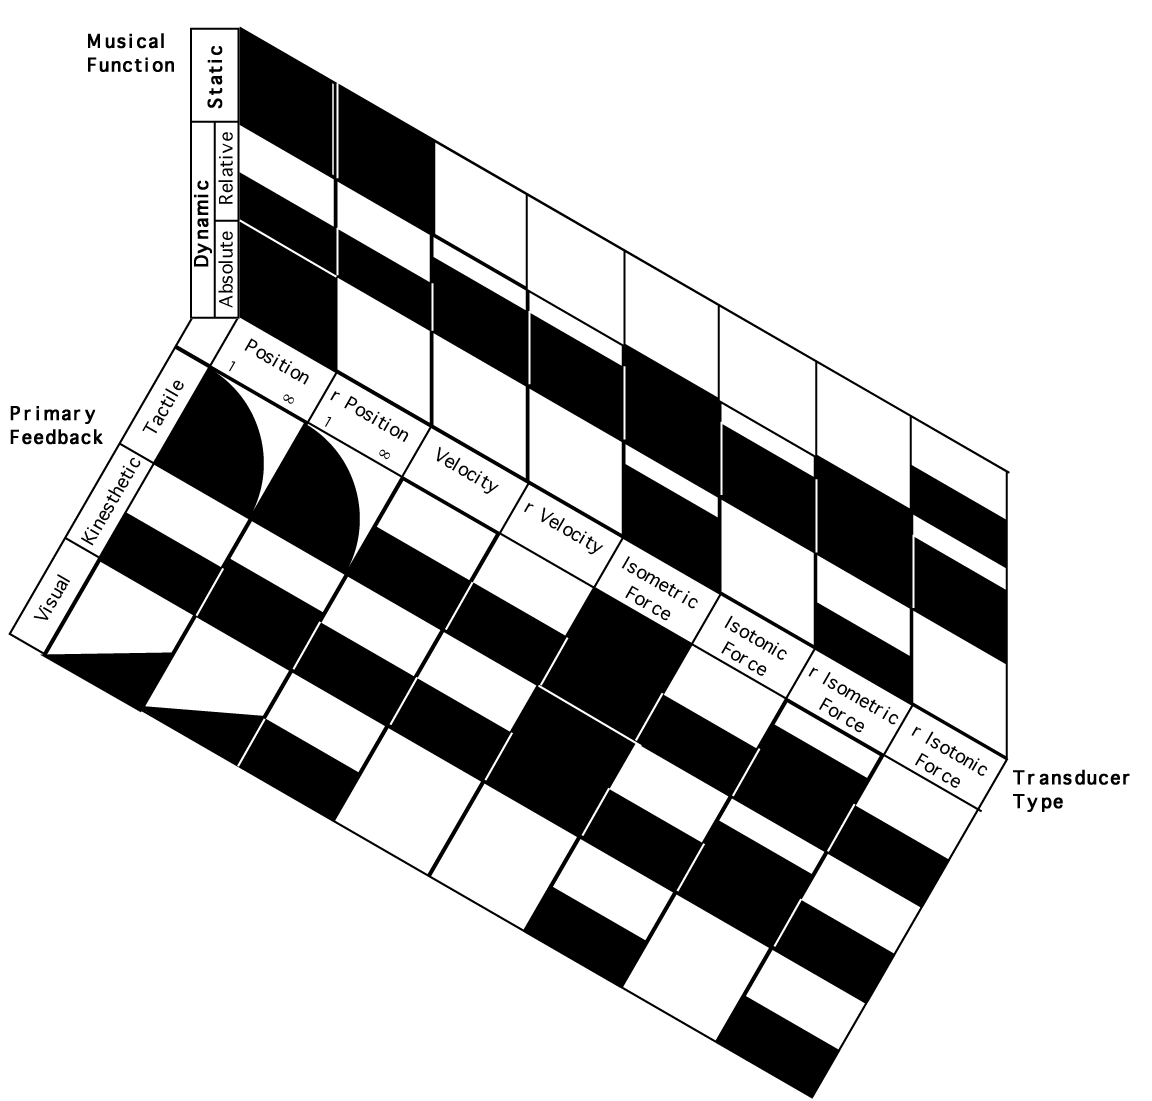
\includegraphics[width=\textwidth]{gfx/05_interfaces/vertegaal-musical-function.png}
	\caption[Adéquation entre fonction musicale, transducteur et retour primaire]{Adéquation entre fonction musicale, transducteur et retour primaire, selon \cite{vertegaal_towards_1996}.}
	\label{fig:interface:vertegaal-transducer-function}
\end{figure}
%-------------------------- Figure : Vertegaal-transducer-function ----------------------------------
\indent Ainsi d'après l'étude de Vertegaal (cf. figure \ref{fig:interface:vertegaal-transducer-function}), un potentiomètre linéaire serait très adapté à la sélection d'une valeur absolue de hauteur, tandis qu'un capteur de pression isotonique tel qu'un \gls{FSR} serait plus adapté à sa modulation. La validité de ce modèle ``subjectif'' (selon les termes des auteurs\footnote{Cf. \cite{ungvary_cognition_1999}}) a été confirmée expérimentalement par une étude récente \footnote{Cf. \cite{malloch_design_2019}}, mais dans un contexte de laboratoire et non un contexte musical réel. Il est ici intéressant de remarquer qu'un clavier de synthétiseur implémente quasiment l'exact opposé de la recommandation sus-mentionnée, en permettant de sélectionner des hauteurs absolues par un ensemble de capteurs de pression et de vélocité sous les touches, tandis qu'un potentiomètre rotatif --~mais présenté latéralement, ce qui rend sa course longitudinale plutôt que radiale~--, le ``\textit{pitch-bend wheel}'' permet leur modulation relative. La différence par rapport au modèle thérorique d'Ungvary et Vertegaal tient au fait que le mapping n'y est pas \textit{one-to-one} en ce qui concerne la hauteur, que le potentiomètre du \textit{pitch-bend-wheel} est muni d'un ressort de rappel et que ces deux capteurs contrôlent la hauteur de manière conjointe.\\
%-------------------------- Figure : table du luthier numérique ----------------------------------
\begin{figure}[!htbp]
	\captionsetup{format=plain}%
	\includegraphics[width=\textwidth]{gfx/05_interfaces/clavier-Martenot-MIDI.png}
	\caption[Agencement des capteurs et fonction musicale]{Un exemple de l'influence de l'agencement des capteurs sur leur usage musical: à gauche l'Onde Martenet: slider linéaire pour le contrôle de hauteur (avec la bague) et capteur de pression pour la modulation (d'intensité). A droite, un clavier MIDI : multiples capteurs de pression pour la sélection de la hauteur absolue et potentiomètre pseudo-linéaire pour la modulation (pitch-bend). Photographie de l'Onde Martenot : Wikipedia User:30rKs56MaE}
	\label{fig:interface:martenot-clavier}
\end{figure}
%-------------------------- Figure : table du luthier numérique ----------------------------------
\indent On voit donc que l'usage, la taille, l'agencement des capteurs et le traitement de ses données contribuent pour autant, sinon davantage, à définir les relations entre capteurs et paramètres musicaux, que la nature de la variation du capteur lui-même. Le fait qu'un paramètre musical ne soit pas ``facilement'' modulable avec un certain type de capteur ne présage donc pas de l'inadéquation de ce capteur pour le contrôle du paramètre en question. Tout au contraire, cela peut faire partie de la \textit{raison d'être} de l'instrument, dont la pratique s'apparente parfois davantage à celle du domptage d'un animal sauvage que celle de l'utilisation d'une machine docile\footnote{On pense par exemple au Theremin, sur lequel le contrôle de la hauteur par la distance de la main à l'antenne est très instable et difficile, et dont la maîtrise est probablement un des intérêt de sa pratique.}.

\subsection{Ordinateurs et DSP}
\label{sec:interfaces:computers_and_dsp}

\noindent Si les algorithmes d'un \gls{DMI} sont virtuels, les ordinateurs qui les font tourner sont bien réels et physiques. La principale remarque que l'on puisse faire à leur sujet, concernant leur aspect matériel, est la prodigieuse chute de leur coût et de leur dimensions, depuis leur invention. Une conséquence directe de leur prix abordable a été leur démocratisation, et la conséquence de leur miniaturisation, leur intégration progressive dans des objets mobiles\footnote{Le smartphone en est un exemple significatif, qui a notamment permis le développement d'instruments autonomes tournant sur smartphone; voir par exemple le projet SmartFaust et la pièce pour smartphones de Vincent Carinola: \url{https://youtu.be/cGZB44KI9Y0}}. On peut distinguer dans cette évolution, cinq périodes d'une quinzaine d'années chacunes, résumées dans le tableau \ref{table:computer-size}, la dernière en date étant couramment désignée comme celle de ``l'Internet des Objets'' (IoT, \textit{Internet of Things}).\\
\indent Si l'audionumérique temps-réel a depuis son origine été incarné par des dispositifs dans lesquel l'ordinateur, trop volumineux et lourd, était séparé de l'interface, cette dernière évolution est tout particulièrement intéressante en ce qui concerne les \glspl{DMI}. Elle augure la possibilité pour un public élargi de créer ses propres \glspl{DMI} intégrant interface de jeu et partie computationnelle dans un seul et même objet portable et (re)programmable. Des cartes électroniques comme \textit{Bela} ou \textit{The Owl}\footnote{Bela: \url{https://bela.io}; The Owl: \url{https://www.rebeltech.org}} et des langages comme \gls{FAUST} développé par le \gls{GRAME} \cite{orlarey_faust_2008} ou SOUL annoncé par Roli\footnote{Announced at the Audio Developer Conference 2018. \url{https://youtu.be/-GhleKNaPdk}} reflètent cette tendance.

\begin{table}[!htbp]
	\renewcommand{\arraystretch}{1.1}
	\captionsetup{format=plain}%
	\centering
 	\begin{tabularx}{\linewidth}{
 	>{\hsize=.9\hsize}X% 10% of 4\hsize 
 	>{\hsize=.6\hsize}X% 30% of 4\hsize
 	>{\hsize=.6\hsize}X% 30% of 4\hsize 
 	>{\hsize=1.4\hsize}X% 30% of 4\hsize
 	>{\hsize=1.5\hsize}X% 30% of 4\hsize
       % sum=4.0\hsize for 4 columns
       }
    \hkrule{1.2pt}
	\textbf{Période} &  \textbf{Nom} & \textbf{Taille} 	&  \textbf{Public} 	& \textbf{Audio}	\\
	\hline
	1950~--~1965 	& macro-	& salle		& laboratoires 		& non temps-réel 			\\
	1965~--~1980	& mini-  	& meuble 	& entreprises  		& contrôle temps-réel 		\\
	1980~--~1995	& micro- 	& caisse 	& foyers 			& temps-réel sur \gls{DSP} 	\\
	1995~--~2010 	& laptop 	& livre 	& individus			& temps-réel sur PC 		\\
	2010~--			& nano- 	& < main 	& plusieurs/individu	& temps-réel sur mobile 	\\
    \hkrule{1.2pt}\\[-10pt]
  \end{tabularx}
	\caption[Évolution de l'ordinateur : taille, accessibilité et capacités audio]{Évolution de l'ordinateur  : taille, accessibilité et capacités de calcul audio.}
	\label{table:computer-size}
\end{table}



\subsection{Feed-back: actionneurs}


\noindent En ``sortie'' de la machine, à l'autre extremité de la boucle instrumentale --~si l'on peut dire~-- se trouvent les systèmes qui font le travail inverse des capteurs en venant \textit{agir} sur l'espace sensible. Là encore, de nombreux types d'actionneurs existent pour agir sur diverses dimensions, quoique celles qui nous intéressent plus directement dans le contexte musical soient celles du son, du mouvement et de la lumière (dans la mesure où l'expérience musicale est aussi une expérience \textit{gestuelle}\footnote{Cf. la notion de ``perception gestuelle'' qui recouvre le toucher et les différents aspects proprioceptifs dans \cite{cadoz_synthese_1981}} et visuelle du mouvement).\\
\indent D'un point de vue matériel, l'actionneur se présente comme un composant électronique connectable à l'ordinateur, généralement au moyen d'un \gls{CAN} et d'un amplificateur (parfois intégrés), qui adaptent le signal numérique au courant et voltage adaptés au transducteur. Le transducteur convertit ce signal électrique en oscillations acoustiques, en mouvements mécaniques, en intensités lumineuses, en champs électro-magnétique, etc.\\
\indent L'actionneur n'est toutefois jamais utilisé ``nu'' (sinon dans un modèle théorique erroné) mais toujours couplé à un support matériel qui filtre, amplifie, oriente la diffusion des mouvements de l'actionneur pour les rendre perceptibles. Par exemple, un haut-parleur est inséré dans une enceinte qui oriente la diffusion du son vers l'avant de l'enceinte; ou encore, un écran de vidéoprojection reçoit la trace lumineuse émise par un vidéoprojecteur.\\
\indent Les caractéristiques du matériau auquel l'actionneur est couplé peuvent ainsi considérablement influer sur le résultat sensible de l'action du capteur. Ainsi, un casque audio traduit le signal numérique en une vibration acoustique de manière relativement ``plate''\footnote{C'est à dire sans distordre le signal, ni en fréquence, ni en amplitude, ni dans le temps.} et directe à l'oreille, alors que ce même signal audio-numérique envoyé dans la corde d'une guitare via un transducteur tactile laissera entendre la résonance de la corde, de la caisse de guitare et du lieu (si par exemple on se trouve dans une salle de concert, plutôt que dans une chambre anéchoïque). De même, les rayons lumineux émis par un vidéoprojecteur pourront être envoyés sur des objets complexes (e.g. un bâtiment, ou de la fumée) qui transformeront la qualité du signal émis.\\
\indent La disposition spatiale des actionneurs joue également un rôle qu'il faut prendre en compte, car leurs actions peuvent selon les cas se complémenter (e.g. une image vidéo composée de plusieurs écrans juxtaposés, un front d'onde recréé par de multiples haut-parleurs dans la \gls{WFS}, etc.), interférer (e.g. l'opposition de phase qui créé des ``trous'' dans le spectre sonore quand des signaux harmoniques en phase synchrones sont envoyés sur plusieurs haut-parleurs) ou entrer en résonance (e.g. l'effet larsen résultant d'une boucle capteurs entre actionneurs se contrôlant et s'influençant mutuellement). La possibilité de pouvoir facilement assigner, sur ordinateur, des relations de correspondances entre n'importe quel type de capteur et n'importe quel type d'actionneur entraîne la possibilité de larsens multi-modaux : par exemple un système dans lequel le son est capté par un microphone, utilisé pour générer une image, l'image utilisée pour générer du son, capté par le microphone.)\\
\indent En dernier lieu, si l'on peut envisager une action directe des actionneurs sur notre perception, sans médiation intermédiaire \footnote{Ce qui est le cas dans des dispositifs tels que la projection rétienienne, les implants cochléaires ou neuronaux}, il faut encore considérer les effets de notre perception, qui filtre, amplifie, focalise, elle aussi les signaux que nous recevons, et s'ajoute à la médiation complexe qui opère entre la représentation numérique du signal sur l'ordinateur et la perception du phénomène sensible provoqué par les actionneurs.\\
\indent En dernier lieu, si l'on peut envisager une action directe des actionneurs sur notre perception, sans médiation intermédiaire \footnote{Ce qui est le cas dans des dispositifs tels que la projection rétienienne, les implants cochléaires ou neuronaux}, il faut encore considérer les effets de notre perception, qui en plus de filtrer, d'amplifier, de focaliser elle aussi (comme un matériau) discrimine, ordonne, interprète, construit, aime ou rejette les signaux que nous recevons, en s'ajoutant à la médiation complexe qui opère entre la représentation numérique du signal sur l'ordinateur et la perception du phénomène sensible provoqué par les actionneurs.\\
\indent Outre les caractéristiques techniques de l'actionneur (puissance, bande passante, course, etc.), il faut donc ainsi prendre en compte les propriétés des matériaux auquel les actionneurs sont couplés, en y incluant les processus cognitifs à l'œuvre dans la perception de leur action sur le sensible\footnote{L'étude des propriétés acoustiques des matériaux ainsi que des mécanismes de la psychologie cognitive mène par ailleurs à l'élaboration de modèles utilisables dans les lutheries numériques. Cf. section \ref{ch:algorithms:digital-material:models}}. À défaut, s'intéresser à ces caractéristiques prises isolément risque de conduire à oublier leur articulation dans l'instrument lui-même, comme le note François Dumeaux : \iquote{Quand tu composes par exemple une pièce, combien de fois je me suis retrouvé à aligner des belles courbes ... c'était pas avec les oreilles que je faisais ma courbe de volume, c'était avec mes yeux. Voilà, (...) tu te retrouves à faire des trucs absurdes, à être tatillon... [à dire, en parlant des valeurs MIDI de la courbe] ``ah non c'était à 127!'',  alors qu'en fait on n'entend pas la différence...} (entretiens personnel, cf. Annexe \ref{appendix:dumeaux}).

%%%%%%%%%%%%%%%%%%%%%%%%%%%%%%%%%%%%%%%%%%%%%%%%%%%%%%
\section{La part acoustique de l'interface des DMIs}
\label{sec:interfaces:part_acoustique}

\noindent Il faut ici rappeler que les \glspl{DMI}, s'ils se caractérisent par l'usage de la computation numérique, sont aussi nécessairement des instruments électroniques, électriques et acoustiques. Il portent l'héritage et les contraintes propres à ces différents médias. Mais le phénomène acoustique, omnidirectionnel et tri-dimensionnel dans le monde physique, est réduit dans l'électronique numérique à un signal mono-dimensionnel\footnote{Nicolas Collins, dressant une liste de traits distinctifs entre hardware et software dans \cite{collins_semiconducting_2013} notait: ``Traditional acoustic instruments are three-dimensional objects, radiating sound in every direction, filling the volume of architectural space like syrup spreading over a waffle. Electronic circuits are much flatter, essentially two-dimensional. Software is inherently linear, every program is a one-dimensional string of code.''} et mono-directionnel\footnote{Au niveau logiciel, des blocs bi-directionnels de plus haut niveau peuvent cependant être crées, comme par exemple dans la librairie de modèles physiques pour \gls{FAUST}, cf. \cite{berdahl_introduction_2012} et \cite{michon_faust_2018}.}, introduisant une distinction entre les ``entrées'' d'une part et les ``sorties'' d'autre part. La dimension acoustique des \glspl{DMI} s'intègre donc dans un circuit ouvert ou fermé avec le système de computation via des transducteurs acoustiques --~microphones en entrée, ou haut-parleurs en sortie.\\
% \indent Par ailleurs, la vibration acoustique peut-être ressentie de manière auditive, quand sa transmission est aérienne, ou tactile lorsqu'elle est solidienne. Ces deux types de vibrations correspondent généralement à deux technologies de transducteurs différentes.

\subsection{Captation : microphones et transducteurs piezo}

\noindent La captation en direct de son acoustique dans un instrument électronique est une pratique très courante chez les musiciens électroacoustiques, et permet des séquences de jeu en prise directe avec des sons concrets, amplifiés, enregistrés, transformés par l'instrument (ou non). En particulier, l'usage de microphones, notamment de transducteurs piezo dits ``microphones de contact'', vient redonner une composante acoustique au corps physique de l'agencement instrumental (et du musicien s'il utilise directement sa voix et son corps), cette composante acoustique ``naturelle'' étant sinon généralement couverte par la puissance du son amplifié. L'intérêt principal réside dans la richesse du signal capté, comme le note Miller Puckette\footnote{``(...) sliding a brush over a drum trigger isn’t likely to produce  anything  useful,  whereas  doing  the  same  thingon an instrument that operates directly on the audio signal from the contact microphone (as we do here) has the possibility to create a wide range of useful musical sounds.'' \cite{puckette_infuriating_2011}.} : \iquote{(...) il y a peu chance que le frottement de balais sur un pad de batterie produise quoi que ce soit d'intéressant, alors que faire la même chose sur un instrument qui fonctionne directement avec le signal audio du microphone de contact (...) offre la possibilité de créer une large gamme de sons musicaux utiles.} L'usage d'algorithmes d'analyse en temps-réel permet, au-delà d'effets déjà existants dans le domaine électroacoustique, d'utiliser les caractéristiques du son comme paramètre de contrôle\footnote{L'interface Mogees est par exemple principalement basée sur ce principe (\url{https://www.mogees.co.uk}), voir également l'Annexe \ref{appendix:zamborlin}.}. Plusieurs stratégies sont possibles, consistant à utiliser le signal comme source d'excitation de modèles physiques (\cite{momeni_composing_2005, schlessinger_kalichord_2009, mehes_virtual-acoustic_2017, williams_pitch_2017, robertson_harmonic_2018}), de filtrages convolutifs (\cite{schwarz_rich_2014}), ou encore d'utiliser des paramètres de plus haut niveau extraits du signal. En particulier, le suivi temps-réel de pitch, s'il reste un problème ouvert dans le domaine des \gls{MIR}, bénéficie d'une histoire de plus de 40 ans (\cite{noll_cepstrum_1967}) et de nombreux algorithmes relativement efficaces sont disponibles (\cite{boersma_accurate_1993, de_cheveigne_yin_2002,pardue_low-cost_2015, schramm_polyphonic_2018}). Le suivi de hauteur (ainsi que d'autres caractéristiques du son) a été particulièrement développé à l'\gls{IRCAM} et est utilisé en concert, depuis le développement d'Antescofo\footnote{\label{fn:interface:antescofo} Antescofo est la dernière version des systèmes de suivi de partition développés à l'\gls{IRCAM}. Au-delà du suivi, Antescofo intègre par ailleurs un système de programmation synchrone qui permet de synchroniser des événements (e.g. musicaux) avec des motifs repérés dans ce qui est capté par le système.}, dans de nombreuses pièces mixtes pour instruments acoustiques captées en temps-réel\footnote{Un exemple en est la pièce \textit{En Echo} de Philippe Manoury, une des premières pièces utilisant un suivi audio temps réel (sur la voix), ainsi que l'extraction des hauteurs des différents formants de la voix pour contrôler la synthèse.}.


\subsection{Diffusion : haut-parleurs et transducteurs tactiles}

\noindent Dans le cas le plus trivial, l'acoustique des \glspl{DMI} se limite à la membrane du haut-parleur qui transforme \textit{in fine} le signal audio-numérique en son acoustique\footnote{Le choix des haut-parleurs peut jouer un rôle primordial, comme c'est le cas dans la musique acousmatique diffusée sur orchestre de haut-parleur ou ``acousmonium''. Voir en particulier \cite{mooney_sound_2006}}. À la différence des instruments acoustiques, la diffusion et la projection du son est souvent séparée de l'interface gestuelle et, bien souvent, distante du musicien quand elle est ``spatialisée''. La spatialisation du son a en effet joué un rôle essentiel dans la motivation des concerts électroacoustiques ``live'', à une époque où l'arrivée du \gls{CD} est vendue comme la possibilité d'une écoute de salon ``haute-définition'' équivalente à l'expérience du concert\footnote{Comme en témoignent les publicités de l'époque, par exemple celle de Phillips mettant en scène un public les yeux bandés incapables de faire la différence entre le concert et l'écoute d'un \gls{CD}: \url{https://youtu.be/jtNyWmD3EQ4}}, comme le raconte Serge de Laubier en parlant des origines du PSO\footnote{``Processeur Spatial Octophonique'', système de spatialisation inventé par De Laubier en 1986.} et du Méta-Instrument dans les années 1980 : \iquote{Si on entend mieux chez soi, c'est pas la peine de faire des concerts, donc il faut qu'au concert, il y ait une expérience unique qui vaille le coup de se déplacer, d'où réfléchir à un système de spatialisation.} (communication personnelle, cf. annexe \ref{appendix:delaubier}).\\
\indent Mais le retour acoustique peut également être perçu dans sa dimension tactile. Verillo montre que la sensibilité du doigt est capable de perçevoir des vibrations jusqu'au kHz \cite{verillo_vibration_1991} et dans les années 1990 plusieurs \glspl{DMI} explorent les possibilités offertes par un retour vibrotactile dans l'interface de jeu \cite{chafe_tactile_1993, bongers_tactual_1998}. Au début des années 2000, plusieurs études propose une analyse de tels dispositifs à la fois sous l'angle technique et dans la perspective de leurs usages dans les \glspl{DMI} (e.g. \cite{rovan_typology_2000, marshall_vibrotactile_2006, birnbaum_towards_2005}). L'essor progressif des transducteurs tactiles à large bande audio depuis la dernière décennie a renouvellé l'intérêt pour le vibrotactile en permettant de l'associer directement au retour audible via le rayonnement acoustique d'un matériau support, comme c'est le cas dans les instruments augmentés à contrôle actif tels que la \textit{Smart Guitar} de HyVibe\footnote{\label{fn-hyvibe}\url{https://www.hyvibe.audio}}. Ce retour vibro-acoustique présente plusieurs intérêts :
\vspace{-1em}
\begin{itemize}[noitemsep]
	\item \textbf{offrir au musicien un retour vibratoire} (et/ou auditif), qui lui permet de mieux ressentir le résultat sonore et pouvoir plus facilement identifier sa contribution personnelle dans le cas de musique d'ensemble\footnote{Voir par exemple les systèmes \textit{SubPac} (\url{https://subpac.com}), ou \textit{Basslet} (\url{https://lofelt.com}) commercialisés pour augmenter la perception du son par la vibration tactile.};
	\item \textbf{faciliter l'identification et la localisation} auditive des instruments et accroître la lisibilité des relations geste/son pour le public;
	\item \textbf{bénéficier des propriétés acoustiques des matériaux} structurels de l'instrument, notamment leur rayonnement, beaucoup plus singulier que celui des haut-parleurs (dont la conception est généralement orientée vers un rayonnement homogène et une bande-passante plate);
	\item \textbf{introduire du feedback} dans le corps de l'instrument en recaptant cette vibration. Traité avec une latence suffisamment faible, cette possibilité laisse la possibilité de transformer dynamiquement les propriétés acoustiques des matériaux, comme le fait par exemple le système HyVibe\footref{fn-hyvibe};
	\item \textbf{communiquer des informations} à l'instrumentiste via un retour vibratoire, tel que le frettage virtuel\footnote{cf. infra, section \ref{sec:audio-fretting}}, ou des informations sémiotiques de plus haut-niveau\footnote{Voir en particulier le travail de Gabriela Patiño-Lakatos et al. \cite{patino-lakatos_paradigmes_2019} sur la communication intersubjective d'information par voie vibrotactile.}.
\end{itemize}

\subsection{Boucler la boucle}

\indent Paradoxalement, si le résultat acoustique d'un instrument est \textit{in fine} ce qui nous intéresse le plus, la part acoustique de l'instrument numérique est aussi la plus problématique. Sur un instrument acoustique, le contrôle du son se fait directement, de manière haptique. Il est ainsi possible d'exciter un élément résonant (e.g. une corde ou une peau) et d'étouffer sa résonance en appliquant simplement la main sur les éléments résonants. La surface du résonateur, qui présentent un nombre infini de modes de résonance, permet de plus d'interagir directement avec tous ces modes. Par exemple, on peut sélectionner des harmoniques sur une guitare en positionant son doigt sur un nœud de vibration du mode en question, ou encore obtenir un timbre ``étouffé'', filtré de ses modes d'ordre élevé par une technique de \textit{palm-muting} sur l'extrémité des cordes d'une guitare. C'est une manière très intuitive d'agir avec le timbre d'un instrument de manière tangible.\\
\indent Dans le cas où le système microphone/DSP/haut-parleur est non-bouclé (typiquement, quand les haut-parleurs sont éloignés des microphones), on contrôle facilement le filtrage de la source, sans que posent de vrais problèmes de stabilité, ce qui permet d'appliquer toute sorte de transformations actives ou passives, linéaires ou non.\\
\indent Dans le cas où les haut-parleurs et microphones ne sont plus distants, mais intégrés à l'interface, les effets de feedback rendent les traitements beaucoup plus instables. La stabilité globale nécessite que le système électronique soit l'équivalent d'un système physique analogique\cite{berdahl_feedback_2012}, ce qui contraint fortement l'espace des transformations possibles et constitue un problème de traitement du signal ouvert\footnote{Voir notamment les travaux de S3AM de l'\gls{IRCAM} sur ce sujet : \cite{muller_power-balanced_2018, falaize_passive_2018, muller_minimal_2019}}. La recherche dans le domaine du ``contrôle actif'' qui s'intéresse précisément aux possibilités de modification dynamique des propriétés acoustiques d'un matériau physique, a développé ces dernières décennies un ensemble de modèles \cite{boutin_active_2011, benacchio_mode_2015, meurisse_active_2015, pardue_separating_2019} et de techniques pour faire face à ce problème, sans l'avoir totalement résolu. Essentiellement, il s'agit de soustraire la contribution de l'actionneur au signal capté par le microphone d'une part en échantillonant à haute fréquence, de traiter le signal avec une latence la plus faible possible, et de n'utiliser que des filtres linéaires passifs pour éviter un repliement spectral qui pourrait faire diverger le signal.\\
\indent A défaut d'une solution idéale, l'utilisation de microphones et de transducteurs acoustiques dans le corps physique de l'instrument reste une option intéressante tant au niveau sonore qu'au niveau tactile, sans nécessairement nécessiter une stabilité absolue du système. On peut ici tirer partie du fait que les gains en entrée comme en sortie peuvent être ajustés dynamiquement (et donc, être ``joués'' comme d'autres paramètres), soit pour utiliser alternativement le microphone et le haut-parleur, soit pour jouer de leur instabilité conjointe. Dans ce dernier cas, l'usage de filtres et de compresseur (notamment) permet de garder l'amplitude et la fréquence du signal dans une zone non-douloureuse de l'audition, et même, une zone riche en qualité de timbre. C'est cette solution pratique qui a été utilisée dans le développement du Filigramophone et du Xypre.


%%%%%%%%%%%%%%%%%%%%%%%%%%%%%%%%%%%%%%%%%
\section{Ergonomie, ergodynamisme}
\label{sec:interfaces:ergonomy}

\subsection{Portabilité de l'interface}
\label{sec:interfaces:ergonomy:portability}

\noindent Avant d'évoquer l'ergonomie de l'instrument en situation de jeu, notons ici que l'instrument (et l'instrumentiste) a une vie en dehors de son usage musical sur scène. Le musicien est amené à [faire] transporter son instrument, à pied, en métro, en voiture, en camion, en avion... Le hardware, comme son nom l'indique, est ``dur'', concret, matériel. Son poids et ses dimensions affectent sa transportabilité et constituent un facteur contraignant pour le musicien. Sa dématérialisation dans des alternative logicielles —\textit{soft}, plus douces et légères— permet d'intégrer dans les limites acceptables pour leur transport, certaines fonctionnalités offertes par les équipements \textit{hard}. En particulier, la virtualisation des outils d'ingénierie du son (table de mixage, équaliseurs, compresseurs et autres effets) permet leur intégration dans l'instrument lui-même\footnote{Ainsi, Serge de Laubier qui utilisait jusqu'en 2005 une table de mixage Yamaha O2R (31kg) motorisée et contrôlée directement depuis son Méta-Instrument, ainsi qu'un échantilloneur EMU (4,5kg) a progressivement conçu des émulations logicielles tournant sur un MacBookPro (1.8kg) de ces équipements pour alléger le transport. Pour une analyse approfondie de cette importance critique du poids des \glspl{DMI}, voir l'analyse de John Richards dans \cite{richards_32kg_2006}. Par ailleurs, les émulations logicielles permettent de réaliser d'autres fonctions qui n'étaient pas présentes dans les modèles originaux. De même, voir les propos d'Adrien Mamou-Mani (annexe \ref{appendix:mamou-mani}) sur l'intérêt que trouvent les ingénieurs du son à ce qu'une partie du traitement audio soit pris en charge par l'instrument lui-même}. Cela étant, la part scénographique des instruments fait que leurs dimensions peuvent également être impratiques à dessein\footnote{Le but d'un instrument n'est pas de nous simplifier la vie, alors que l'absence d'effort constitue \iquote{une vertu cardinale dans la mythologie de l'ordinateur} comme le notait Joel Ryan dans \cite{ryan_remarks_1991}.} pour confronter le musicien et le public à un objet hors-norme\footnote{Cf. par exemple le projet ``Machine \_ Variation'' de Nicolas Bernier et Martin Messier, et les observations de Bernier en annexe \ref{appendix:bernier}.}.\\
\indent Les instruments peuvent prendre différentes formes, plus ou moins grandes, qui définissent à la fois leur portabilité ainsi que la posture du musicien envers son instrument. On peut distinguer quatre types de rapport à l'interfaces de jeu impliquant différent rapports de proximité avec l'instrument:
\vspace{-1em}
\begin{itemize}[noitemsep]
	\item \textbf{interfaces portable}, qui \textit{adhèrent} au corps. L'interface est \textit{portée} (comme un habit) et les mouvements du corps sont captés directement et en permanence, par exemples sont le Méta-Instrument 3, The Hands, le Myo d'Atau Tanaka, la guitare électrique, etc.;
	\item \textbf{interfaces portative}, qu'on peut \textit{prendre} et \textit{tenir} dans ses mains pour en jouer, mais également \textit{poser} (comme un ustensile), par exemple ``The Sponge'' de Martin Marier, un tambourin, un gamepad, un harmonica;
	\item \textbf{interfaces statue}\footnote{Claude Cadoz nomme ce type de configuration ``dispositif à vis-à-vis'' dans \cite{cadoz_geste_1994}}: objets trop grands pour être déplacés (où qui n'a pas vocation à) mais autour duquel on peut tourner. L'instrument est \textit{touché} (comme une sculpture), par exemple les claviers, et pad \gls{MIDI}, les ``intonarumori'' de Bernier/Messier\footnote{Voir \url{http://www.lachambredesmachines.com}}, les synthétiseurs modulaires en rack, le Théremin, etc.);
	\item \textbf{interfaces immersives} : captant une variation particulière dans l'intégralité de l'environnement. L'instrument est \textit{enveloppant} (comme un lieu), et joué en étant \textit{parcouru}. Il m'entoure mais je n'ai pas directement accès à lui, par exemple les instruments basés sur caméra ou Kinect, les installations sonores utilisant la réalité virtuelle (CAVEs, etc.);
\end{itemize}
\begin{wrapfigure}[12]{r}{0.44\textwidth}
	\vspace{-1em}
	\captionsetup{format=plain}
	\centering
 	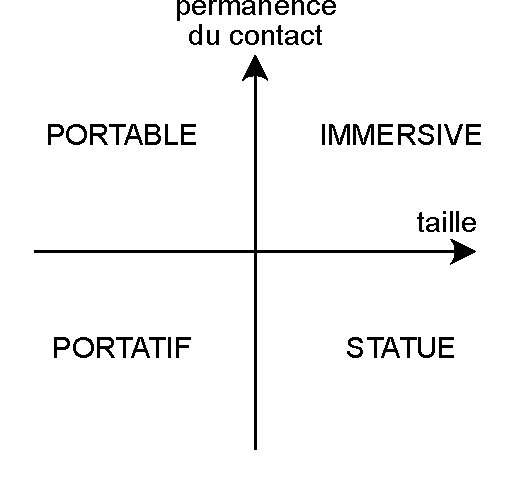
\includegraphics[width=0.4\textwidth]{gfx/05_interfaces/interface-portabilite.pdf}
 	%\vspace{-2em}
	\caption[Portabilité et permanence du contact avec l'interface.]{Portabilité et permanence du contact avec l'interface.}
 	\label{fig:interfaces:portabilite}
\end{wrapfigure}
\par
\noindent Ces catégories ne sont pas étanches; par exemple, un synthétiseur à clavier se jouera aussi bien assis, que debout, que porté en bandoulière dans le cas des \textit{Keytars}\footnote{contraction des termes \textit{keyboard} et \textit{guitar} désignant les synthétiseurs à clavier qui se portent comme les guitares électriques}. On représenterait mieux ces catégories par un espace continu, polarisé par la taille de l'interface en abscisse et la permanence du contact \underline{requis par l'instrument} en ordonnée (figure \ref{fig:interfaces:portabilite}). L'origine des abscisse serait alors un rapport de taille à la limite de ce qu'il est possible de porter, et qui constitue un point de clivage en terme d'usage. L'ordonnée s'étend entre deux extrêmes représentant un contact permanent (tel que dans une installation immersive) et un contact inexistant, ou du moins limité à son activation (instrument autonome).
%-------------------------- Figure : wacom ---------
% \begin{figure}[!htbp]
% 	\captionsetup{format=plain}%
% 	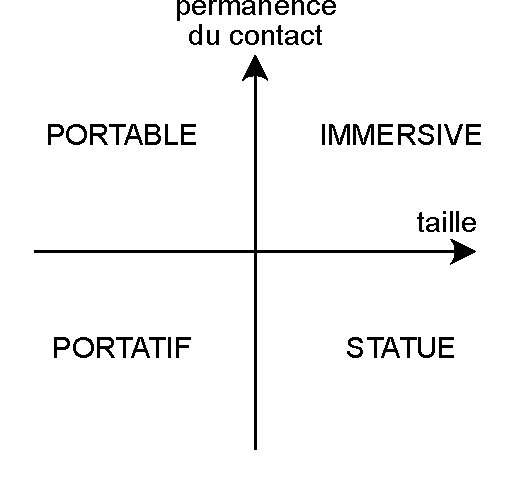
\includegraphics[width=\textwidth]{gfx/05_interfaces/interface-portabilite.pdf}
% 	\caption[Portabilité et permanence du contact avec l'interface.]{Portabilité et permanence du contact avec l'interface.}
% 	\label{fig:interfaces:portabilite}
% \end{figure}


% \setlength\intextsep{12pt}
% \begin{wrapfigure}[16]{r}{0in}
%   ...
% \end{wrapfigure}
% \vspace{-15pt} \leavevmode\section{Section title}
%-------------------------- Figure : wacom ---------


% \begin{table}[!htbp]
% 	\renewcommand{\arraystretch}{1.1}
% 	\captionsetup{format=plain}%
% 	\centering
%  	\begin{tabularx}{\linewidth}{
%  	>{\hsize=1\hsize}X% 10% of 4\hsize 
%  	>{\hsize=1\hsize}X% 30% of 4\hsize
%  	>{\hsize=1\hsize}X% 30% of 4\hsize 
%        % sum=4.0\hsize for 4 columns
%        }
%     \hkrule{1.2pt}
% 	\diagbox{mobilité}{contact}	&  \textbf{permanent} & \textbf{temporaire} \\
% 	\hline
% 	\textbf{immobile} 					& immersif					& sur pied					\\
% 	\textbf{mobile} 							& vêtement  				& outil 			\\
%     \hkrule{1.2pt}\\[-10pt]
%   \end{tabularx}
% 	\caption[Portabilité et contact]{Portabilité et contact.}
% 	\label{table:portabilite}
% \end{table}



\subsection{Disponibilité de l'interface}
\label{sec:interfaces:ergonomy:disponibility}

\noindent L'agencement modulaire des \glspl{DMI} entraîne par ailleurs un temps de démontage-remontage de l'instrument avant qu'il soit possible d'en jouer. Leur fonctionnement nécessite généralement la disponibilité de prises de courant à proximité, voire de réseau WiFi. Il faut ensuite câbler les haut-parleurs distants (pour la spatialisation du son), les capteurs et/ou actionneurs parfois distants eux-aussi (e.g. lors de l'usage de caméra), les machines qui fonctionnent en réseau, et les divers modules (carte son, interface d'acquisition, microphones, boites de direct, etc.) Se rajoute ensuite le ``temps de lancement'', c'est-à-dire le temps de démarrer l'ordinateur, de lancer le(s) logiciel(s) nécessaire(s), d'ouvrir le patch ou le script adéquat, et éventuellement de l'initialiser avec la bonne configuration. S'ajoute enfin le temps prélablement passé (même si les surprises au moment du concert peuvent arriver) à maintenir la partie algorithmique opérationnelle avec les changements d'\glslink{OS}{OS} et les mises à jour logicielles, comme il a été souligné dans le chapitre \ref{ch:ephemeral} et dans l'étude de Morreale et McPherson \cite{morreale_design_2017}.\\
\indent Le terme ``plug'n play'' est couramment utilisé pour qualifier une disponibilité immédiate de l'instrument, mais sur de tels dispositifs, la temps de branchement peut dans les faits s'avérer assez long. Il est important de prendre en compte cette durée dans le design d'un \gls{DMI}, car tout le temps passé sur la partie de montage technique est pris au détriment du temps de jeu\footnote{Cf. les propos de Nicolas Bernier (annexe \ref{appendix:bernier}), François Dumeaux (annexe \ref{appendix:dumeaux}) et Bruno Zamborlin (annexe \ref{appendix:zamborlin}) dans les entretiens.}. Notons toutefois qu'à la différence des instruments acoustiques, les \glspl{DMI} ne nécessitent généralement pas de temps d'accordage et ne sont généralement pas sujets aux conditions de température et d'hygrométrie requérant un ré-accordage et un ``temps de chauffe'', particulièrement pour les cuivres.


%------------------------------------------------------------
\subsection{Se repérer dans l'interface}
\label{sec:interfaces:ergonomy:cues}

\noindent L'apprentissage et la maîtrise d'un instrument passe par une exploration multimodale qui implique l'ensemble de la perception. Les \glspl{DMI} présentent cette particularité par rapport aux instruments acoustiques que la relation de causalité entre une action sur l'interface et la réaction de l'instrument n'est pas \textit{a priori} basée sur un rapport causal obéissant aux lois de la physique, mais sur une relation programmée, qui constitue comme le dit Thor Magnusson \iquote{une théorie de la musique en soi} \cite{magnusson_sonic_2019}, avec ses règles propres et d'éventuels scénarios évolutifs. Cette exploration peut s'appuyer sur un certain nombre de repères, présentés dans cette section.

\subsubsection{Repères visuels}

\noindent Le premier rapport avec un nouvel instrument inconnu est visuel: avant même de sonner, l'instrument exhibe sa structure spatiale, d'éventuels éléments reconnaissables: marqueurs, touches, poignées, symboles, etc. On pourrait parfois presque imaginer la manière dont il va sonner en le regardant : une interface pleine de \textit{pads} présage d'un jeu rythmique tandis que la surface lisse d'une tablette graphique laisse imaginer des sons plus continus et un jeu sur le timbre. Il est fort possible que l'on se trompe en spéculant de la sorte, mais il est difficile d'échapper à ces associations intuitives suscitées par nos expériences passées. Ces différents aspects visuels seront présentés plus en détail dans le chapitre \ref{ch:visual_representation}.

\subsubsection{Repères sonores}

\noindent Les termes de l'exploration sonore ont déjà été en partie présentés dans la section \ref{sec:ephemeral:playing-a-DMI}. La pratique de l'écoute et de la mémorisation des correspondances entre actions sur l'interface et résultat sonore contribue à enrichir son ``solfège de l'audible'' \cite{savouret_introduction_2010} et découvrir comment ces différents points de résonance (ou \textit{sweet spots}) s'articulent topologiquement, voire chronologiquement, sur l'interface de jeu.\\
\indent Notons la possibilité d'utiliser des \textit{earcons}\footnote{Le terme \textit{earcon}, construit comme un jeu de mot à partir du terme ``icon'' (prononcé eye-con en anglais), est un son bref et distinctif utilisé pour représenter un événement spécifique ou pour transmettre une information.} et autres effets sonores venant notifier de l'usage adéquat (ou non) des fonctions offertes par une interface, par exemple les ``pops'' associés à la pression d'un bouton, ou le bruit d'un cadenas qui s'ouvre ou se ferme pour un interrupteur. Les \textit{earcons} sont rarement utilisées dans les \glspl{DMI} en raison de l'interférence évidente avec le son musical. Ils ne sont toutefois pas à exclure, car il reste possible de séparer ces signaux informatifs du signal audio musical (par un retour au casque sur un canal différent par exemple).\\
\indent Il faut noter ici le cas particulier de l'utilisation du sonore pour le guidage de personnes malvoyantes. Les \glspl{DMI} rendent en effet possible l'implémentation d'un système d'assistance vocale\footnote{Les assistants vocaux se sont largement développés depuis la dernière décennie avec l'émergence des smartphones. \textit{VoiceOver} sur iOS et \textit{TalkBack} sur Android permettent ainsi de parcourir quasiment toutes les informations et fonctions disponibles sur l'écran, via des gestes indépendants de la position à l'écran des zones d'information/interaction et une énonciation vocale des fonctions à disposition et de leur valeurs.}
 pour délivrer des informations \textit{ad-hoc} conçernant l'usage de l'instrument. Nous avons implémenté un tel système dans la \textit{Table Sonotactile Interactive} (cf. figure \ref{fig:interface:tableSonotactile}), un dispositif imaginé pour la \textit{Maison des Aveugles}\footnote{La \textit{Table Sonotactile Interactive} fait partie d'un plus large projet : ``La Carte Sonore'' proposé par Anne Maregiano à la Villa Saint Raphaël \url{https://www.mda-lacartesonore.com}} de Lyon par la compositrice Pascale Criton en collaboration avec Hugues Genevois de l'équipe \gls{LAM} et Gérard Uzan, chercheur en ergonomie du handicap.
%------------ Figure : repères statique -----------
\begin{figure}[!htbp]
	\captionsetup{format=plain}%
	\centering
	\begin{minipage}[t]{0.48\textwidth}
		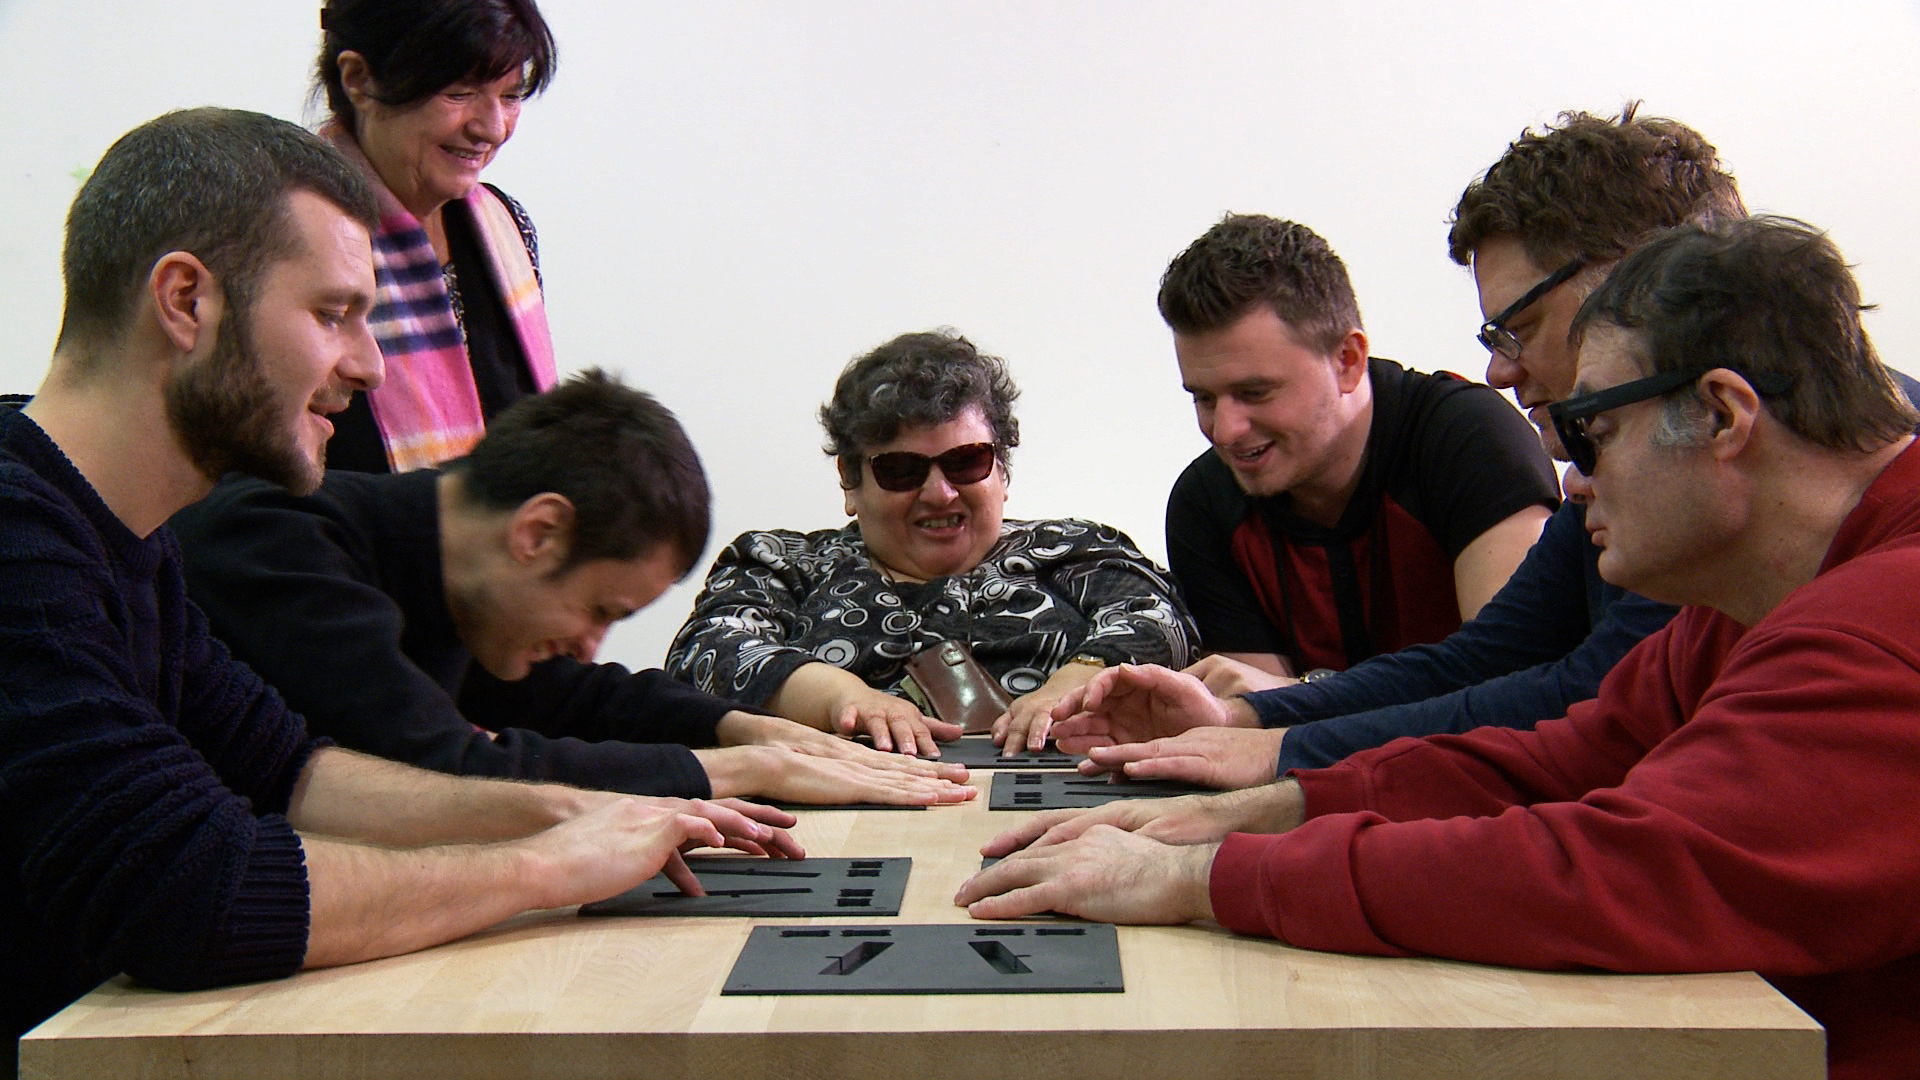
\includegraphics[width=\linewidth]{gfx/05_interfaces/tableSonotactile.jpg}
		\caption[La Table Sonotactile Interactive]{La Table Sonotactile Interactive : un dispositif interactif d'écoute installé à la Maison des Aveugles. Photographie © Anne Maregiano.}
		\label{fig:interface:tableSonotactile}
	\end{minipage}
	\hspace{.02\linewidth}
	\begin{minipage}[t]{0.48\textwidth}
	    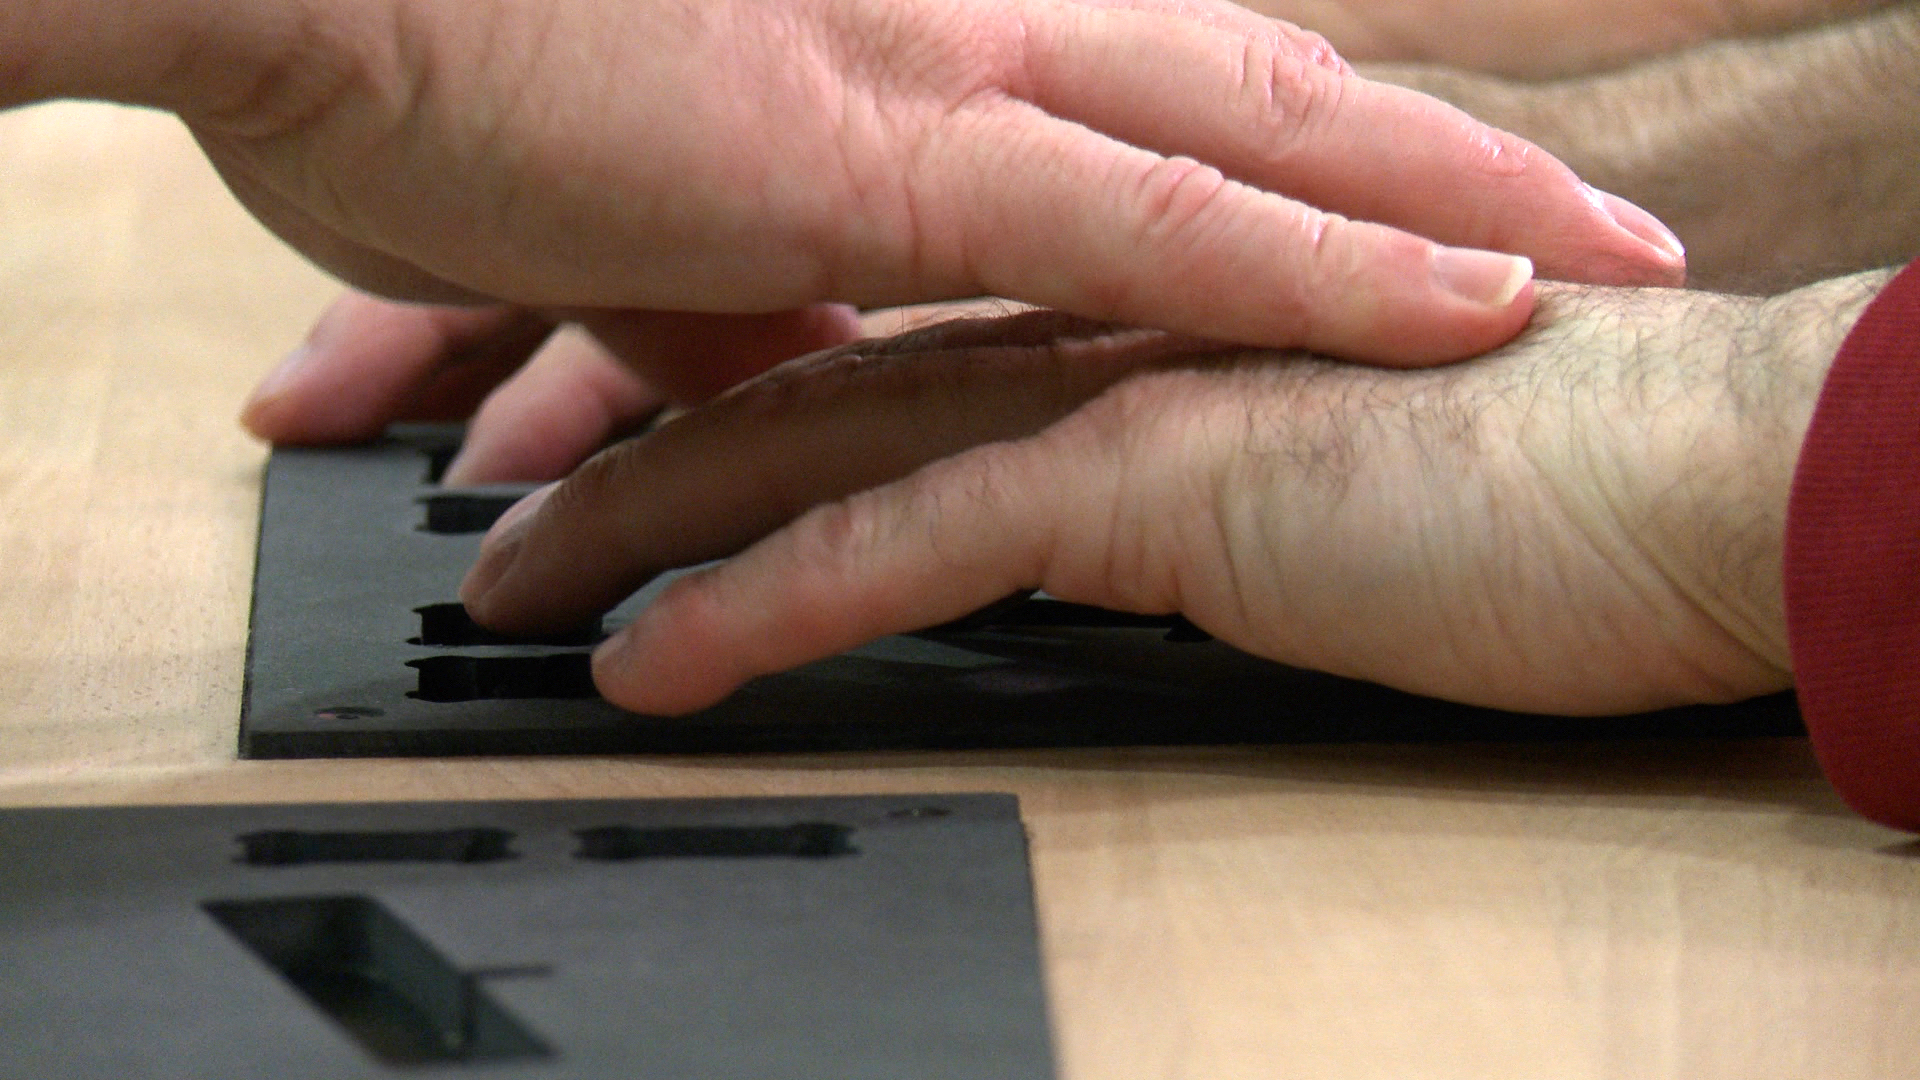
\includegraphics[width=\linewidth]{gfx/05_interfaces/tableSonotactile-pad.jpg}
		\caption[La Table Sonotactile Interactive : détail du pad]{La Table Sonotactile Interactive : détail du pad. Photographie © Anne Maregiano.}
		\label{fig:interface:tableSonotactile-pad}
	\end{minipage}
\end{figure}

\subsubsection{Repères tactiles}

\noindent L'état de surface des matériaux, la présence de reliefs (glissières, concavités, etc.) et de jeux mécaniques (e.g. l'enfoncement élastique d'une mousse recouvrant les pads \gls{MIDI}), contribuent à l'orientation tactile sur l'interface et à augmenter la cohérence entre le sens du toucher et la perception auditive des sons produits par le \gls{DMI}\footnote{Voir par exemple les glissères sur le pad d'interaction de la table sonotactile interactive, qui guident les doigts sur les potentiomètres linéaires, figure \ref{fig:interface:tableSonotactile-pad}}.\\
\indent Un grand défaut des interfaces graphiques dites ``tactiles'' est, ironiquement, que leur surface est généralement dépourvue de tels repères : aucune aspérité ne vient guider la main pour qu'elle trouve son chemin sur la matrice des capteurs, sans l'aide de la vue (ou de signaux sonores, comme vu ci-avant).\\
\indent Différentes stratégies présentées ci-après peuvent venir partiellement compenser cette lacune. Leur application dépend à la fois de la technologie de captation du \textit{multitouch}, ainsi que du type de repère, statique ou dynamique, que l'on souhaite.

\noindent\textbf{\textit{Repères statiques}}\\
\noindent Les surfaces multitouch permettent d'agencer de multiples zones virtuelles d'interaction : l'écran d'un smartphone présentent ainsi des boutons, des sliders, des menus, etc. activant des fonctions dissociées, sans qu'il soit tactilement possible de sentir leur contour. Les interfaces ``Joué''\footnote{\url{https://www.play-joue.com}} ou ``Sensel Morph''\footnote{\url{https://sensel.com}} commercialisent différents revêtements (\textit{overlays}) interchageables pour leur surface \textit{multitouch}. Ces surfaces toutefois dépourvues d'écran graphique, ce qui évacue le problème de la transparence de ces repères. Une solution bon marché consiste à utiliser de la bande adhésive (cf. figure \ref{fig:interface:filigramophone-adhesif}). Un intermédiaire plus fin entre l'éphémère bande adhésive et une solution fixe consiste à utiliser une plaque de \gls{PMMA} (cf. figure \ref{fig:interface:filigramophone-plexigravure}) intermédiaire entre le doigt et la surface tactile, qui permet de graver des motifs potentiellement plus complexes. Cette dernière option n'est toutefois pas toujours réalisable sur les écrans à technologie capacitive, qui nécessite généralement que le doigt soit directement en contact avec l'écran.
%------------ Figure : repères statique -----------
\begin{figure}[!htbp]
	\captionsetup{format=plain}%
	\centering
	\begin{minipage}[t]{0.48\textwidth}
		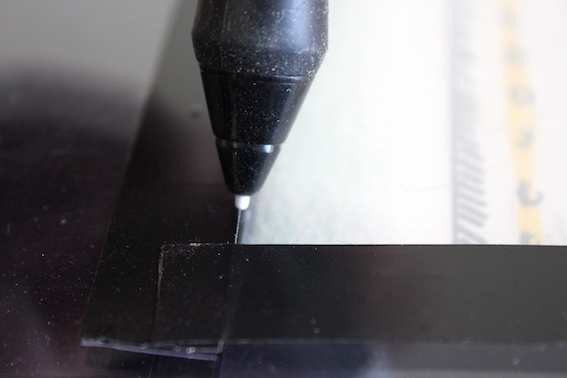
\includegraphics[width=\linewidth]{gfx/05_interfaces/filigramophone-adhesif_72dpi.jpg}
		\caption[Bande adhésive permettant de sentir le contour de la zone sensible de la tablette graphique dans le Filigramophone]{Bande adhésive permettant de sentir le contour de la zone sensible de la tablette graphique dans le Filigramophone.}
		\label{fig:interface:filigramophone-adhesif}
	\end{minipage}
	\hspace{.02\linewidth}
	\begin{minipage}[t]{0.48\textwidth}
	    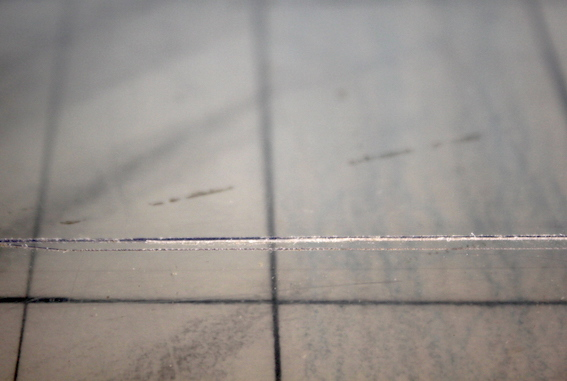
\includegraphics[width=\linewidth]{gfx/05_interfaces/Filigramophone_gravure_72dpi.jpg}
		\caption[Gravure d'une ligne médiane sur la plaque de PMMA du Filigramophone]{Gravure d'une ligne médiane sur la plaque de \gls{PMMA} du Filigramophone.}
		\label{fig:interface:filigramophone-plexigravure}
	\end{minipage}
\end{figure}

%------------ Figure : filigramophone et xypre piezo -----------
\noindent\textbf{\textit{Repères dynamiques : retours haptique et audiotactile}}\\
\label{sec:audio-fretting}

\noindent Les systèmes à retour haptique rendent tangible le contour, la résistance physique ou la vibration d'objets virtuels dynamiques. L'\textit{ACROE} a été pionnière dans cette direction appliquée à la lutherie numérique et développé à la fois des interfaces robotisées ainsi que les logiciels permettant une écriture musicale avec de telles interfaces. Plusieurs projets ont donné lieu à des protoypes d'écrans visuels intégrant un retour haptique, de manière globale \cite{sinclair_touchmover_2013}, ou distribué sur toute la surface par une matrice de mini-actionneurs \cite{follmer_inform_2013}. Des études ont démontré le bénéfice des interfaces haptiques sur l'évaluation qualitative de la relation instrumentale \cite{omodhrain_playing_2001, young_qualitative_2017}, mais la plupart d'entre elles restent encore à l'état de prototype et leur coût ainsi que la complexité de leur conception mécanique constitue souvent un facteur prohibitif.\\
\indent L'accessibilité des transducteurs tactiles, ainsi que la qualité de leur bande passante à considérablement augmenté depuis la dernière décennie et offre une alternative plus souple et économique pour la transmission d'information tactile. La solution la plus simple et directe pour établir un lien entre la perception auditive et tactile consiste à envoyer le résultat sonore (qui serait envoyé sur des haut-parleurs) dans le corps de l'instrument. Cette solution n'ajoute pas \textit{a priori} de repères autres que ceux perçu par les oreilles, mais la sensation vibratoire qui vient se coupler à la perception kinesthésique de gestes génère une sensation complexe perçue comme un tout cohérent, qui fusionne davantage encore que le simple couplage entre l'ouïe et la sensation kinésthésique, et qui semble aider la perception et la mémorisation spatiale de l'instrument. En particulier, utiliser le stylet d'une tablette graphique comme une tête de lecture, en associant sa position sur la tablette à la position temporelle de la lecture d'un échantillon sonore résulte en un troublant renversement des sens : la vibration recréé un état de surface fictif sur l'étendue de la tablette, qui donne l'impression d'être la cause du son entendu. D'autres essais ont été effectués dans la perspective d'améliorer la cohérence entre la sensation tactile et auditive. En particulier, l'accentuation des phénomènes transitoires, par un calcul différentiel du spectre pondéré par une courbe d'isonique, semblait donner de meilleurs résultats. C'est assurément un champ riche et fertile, pour lequel différentes solutions sont envisageables et qu'il conviendrait d'étudier plus en profondeur.\\
\indent Un autre type de repère audiotactile qui s'inspire de cette expérience d'un état de surface virtuel, sans toutefois être aussi directement en relation avec le son audible, consiste à réaliser un ``frettage virtuel'' de la surface de jeu. L'envoi d'impulsions synchronisées à la position du stylet dans un transducteur tactile plaqué sur une tablette graphique, permet de simuler des petites ``bosses'' sur sa surface (un peu comme les frettes sur le manche d'une guitare). Ce frettage peut aider, par exemple, à sentir les paliers dans la progression d'un geste continu (e.g. les différentes ``notes'' d'une échelle de hauteur) (cf. figure \ref{fig:interface:virtual-fretting}) ou les contours d'une zone d'interaction\footnote{Cette technique permettant de simuler un relief par une simple vibration est notamment utilisée depuis 2015 dans les dernières version de boutons d'iPhone et de trackpad sur les ordinateurs portables Apple, une fonctionnalité connue sous le nom ``Force touch''.}.\\

%-------------------------- Figure : wacom ---------
\begin{figure}[!htbp]
	\captionsetup{format=plain}%
	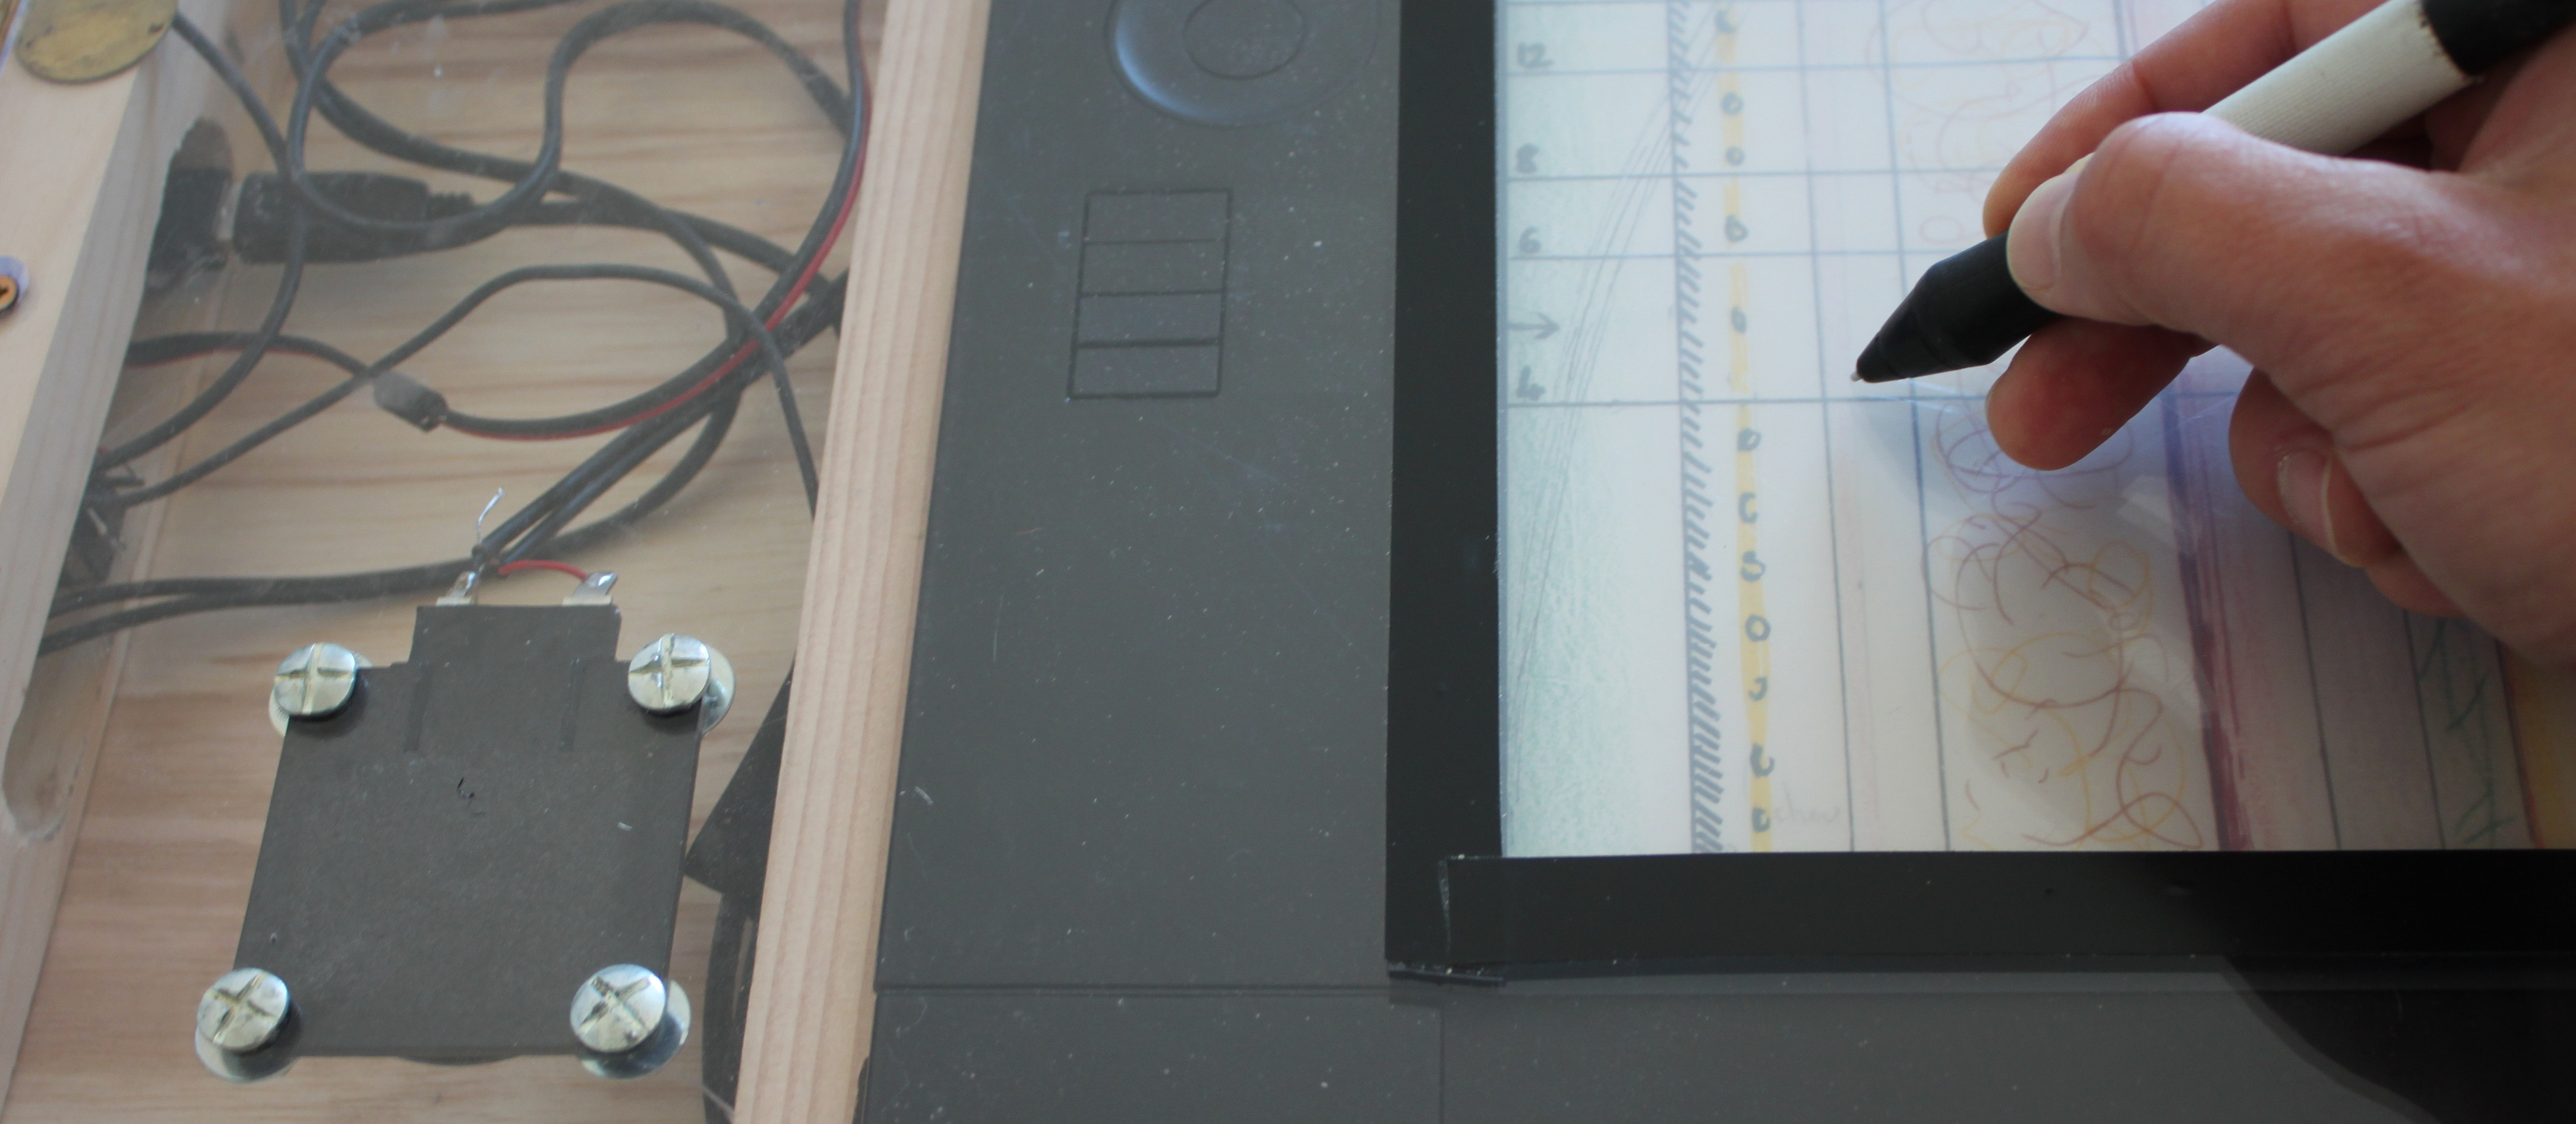
\includegraphics[width=\textwidth]{gfx/05_interfaces/virtual-fretting.jpg}
	\caption[Frettage virtuel par retour vibro-tactile]{Frettage virtuel par retour vibro-tactile: le transducteur tacile (en bas à gauche) émet une impulsion à chaque fois que le stylet franchit une frontière virtuelle (matérialisées par les lignes noires sur le calque).}
	\label{fig:interface:virtual-fretting}
\end{figure}
%-------------------------- Figure : wacom ---------


\noindent\textbf{Anamorphose dynamique}\\
\noindent Enfin, il est possible de procéder algorithmiquement à des anamorphoses de l'espace de jeu. Cette solution ne permet pas de ``créer'' des repères tactiles à proprement parler, mais d'adapter dynamiquement l'espace de l'interaction pour que le geste puisse s'affranchir en partie du besoin de ces repères.\\
\indent Un exemple classique est le vérouillage des composants d'une \gls{GUI} pendant l'interaction: si l'on clique sur un bouton ou un \textit{slider}, l'interaction est maintenue avec le composant tant que le doigt est en contact avec la surface tactile, ce qui permet des gestes plus amples utilisant l'intégralité de la surface de l'écran tactile, plutôt que de les restreindre à une petit zone\footnote{Cette solution a notamment été implémentée dans la librairie mp.TUI présentée au chapitre \ref{ch:visual_representation}}. Cette stratégie d'interaction s'appuie sur la loi de Fitts \cite{fitts_information_1954}, caractérisant \textit{l'indice de difficulté} d'une tâche de selection par pointage, couramment exprimée en terme de temps mis à réussir ce pointage, par la relation (formulation de MacKenzie): 
$$ T = a + b \log_2 (1 + \frac{D}{L})$$
\vspace{-1em}
\begin{conditions}
$T$     	& temps moyen pris pour effectuer le mouvement; \\
$D$			& distance séparant le point de départ du centre de la cible;\\
$L$			& largeur de la cible mesurée selon l'axe de mouvement;\\
$a, b$  	& variables pouvant être déterminés empiriquement.
\end{conditions}

\noindent Un autre exemple d'anamorphose, plus directement lié au domaine musical, est l'algorithme de correction dynamique de la hauteur\footnote{L'algorithme s'applique à la hauteur, comme à n'importe quel autre paramètre qu'il pourrait être intéressant de contrôler à la fois de manière continue et discrètre} à l'attaque, présenté dans \cite{goudard_playing_2014} et sur la figure \ref{fig:algorithms:MID-dynamic-pitch-correction}.

\subsubsection{Repères somesthésiques}

\noindent Enfin, le développement des réflexes moteurs qui permettent la virtuosité de jeu sur une interface passe par une cognition incarnée, qui s'appuie sur notre perception \textit{somesthésique}, c'est-à-dire l'ensemble des sensations internes du corps. En particulier, parmi les différents sensations que recouvrent la somesthésie, la \textit{proprioception} désigne la perception de la position des différentes parties de notre corps dans l'espace, recouvrant le sens du mouvement (\textit{kinesthésie}) et le sens de la posture (\textit{statesthésie}). La somesthésie est particulièrement mise à contribution dans les \glspl{DMI} qui ne présentent pas d'interface physique tangible, tels que ceux basés sur des gestes libres (e.g. captés par une Kinect), et peut s'avérer être la seule sensation directe (i.e. non médiatisée par la machine) disponible dans les \glspl{DMI} basés sur les signaux biologiques (e.g. tension des muscles du Myo).\\
\indent Durant la phase de conception d'un \gls{DMI}, cette exploration est double : il s'agit à la fois d'intégrer la topologie physique de l'instrument (disposition des capteurs, espace du mouvement autour de ceux-ci, course sensible et courbes de réponse...) mais également la topologie virtuelle des algorithmes manipulés, c'est à dire la redistribution dynamique de cette spatialité pendant le jeu musical. Par exemple, dans le cas de la manipulation d'un modèle intermédiaire dynamique\footnote{Cf. section \ref{sec:algorithms:MID}} (e.g. un bâton de pluie virtuel), le résultat d'un même geste pourra différer en fonction de l'état du modèle intermédiaire (selon que les grains de sâble du bâton de pluie sont d'un côté ou de l'autre).\\
\indent Ainsi, le positionnement des capteurs dans l'interface \textit{Xypre} a été revu en fonction de gestes qui venaient naturellement lors du jeu avec le \textit{Filigramophone}. Par exemple, le geste de percussion sur le côté du chassis venait naturellement dans la course du bras pivotant autour de l'articulation de l'épaule, alors qu'aucun capteur n'avait été positionné là. C'est par ailleurs un geste de percussion qu'on retrouve dans des instruments de percussion comme le Mridang indien, et que l'auteur ayant pratiqué le tabla trouvait relativement aisé.

[extra]:\\
correpondance entre l'anatomie corporelle et celle de l'interface\\
\iquote{Though there is a huge range of performer decision, history, and knowledge that will determine their exact method of playing (as established by Jorda [12]), the physical design of the DMI impacts this gesture repertoire by presenting certain affordances.} \cite{bin_hands_2017}


%------------------------------------------------------------
\subsection{Ergodynamie}

\noindent Les différents aspects qui contribuent à l'ergonomie de l'interface de jeu d'un \gls{DMI} sont ainsi à la fois ancrés dans le corps matériel de l'instrument, mais également dans les artéfacts sonores, visuels ou vibratoires produits par l'ordinateur. À ces aspects cognitifs s'ajoute l'expérience personnelle et la reconnaissance de tous les éléments appartenant au répertoire culturel dans lequel un nouveau \gls{DMI}, encore inconnu, s'inscrit.\\
\indent Thor Magnusson propose la notion d'\textit{ergodynamie} \iquote{comme un terme qui s'approche d'une certaine manière de l'usage du mot `gameplay' dans le domaine des jeux vidéo, mais qui traduit également une conscience et une expérience de l'instrument dans des pratiques incarnées, historiques et esthétiques. L'ergodynamie concerne l'objet étudié, mais elle se rapporte aussi bien au contexte culturel qu'à des expériences personnelles subjectives de cet objet.}\footnote{\iquote{(...) the word \textit{ergodynamics} is proposed as a term that somewhat relates to the use of ‘gameplay’ in computer games, but further signifies an awareness and experience of the instrument in embodied, historical, and aesthetic practices. Ergodynamics are of the object studied, but it relates equally to cultural context and subjective personal experiences of it.} \cite{magnusson_ergodynamics_2019}}


%%%%%%%%%%%%%%%%%%%%%%%%%%%%%%%%%%%%%%%%%
\section{Un exemple pratique : phylogenèse d'interfaces de type tablette}
\label{sec:interfaces:phylogenese}

\noindent Cette partie retrace le développement d'une série d'interfaces de \glspl{DMI}, basée sur un archétype d'instrument de type ``tablette''. On peut voir dans la tablette graphique des liens évidents avec les gestes du dessin et de l'écriture, tandis que l'usage généralisé des écrans \textit{multitouch} sur les smartphones a fait émergé un grand nombre d'habitudes d'interaction (ainsi que les attentes que ces habitudes génèrent) telles que les mouvements de balyage, de \textit{pinch-to-zoom}, de défilement à deux doigts, etc.\\
\indent La conception d’une nouvelle interface pour la performance musicale est une tâche complexe, nécessitant de nombreux aller-retours entre conception, fabrication et pratique musicale. Le filigramophone est une interface qui a connu plusieurs versions, suffisamment différentes pour les considérer comme des instruments distincts et suffisamment similaires pour y voir la continuité d’une seule et même famille d'instruments.

%----------------------------------------------------------------------------------------------------------
\subsection{Origine : la tablette graphique (2005)}
\label{sec:interfaces:phylogenese:wacom}

\noindent La tablette graphique (précisément un modèle Sapphire de Wacom) a été l’interface originelle qui a servi de base au filigramophone. J’ai commencé à l’utiliser dans le cadre du développement de la Méta-Mallette\footnote{Logiciel pour la pratique collective de musique par ordinateur développé par l’association Puce Muse, au développement duquel j'ai activement participé entre 2005 et 2008.}. Le choix de cette interface était motivé par la diversité de gestes expressifs possibles sur une tablette graphique, ainsi que par son coût relativement abordable\footnote{un peu moins de 100€ en 2005, autour de 50€ pour un modèle équivalent en 2019.} comparativement à la plupart des interfaces \gls{MIDI}, permettant de la déployer en nombre, dans le cadre d'activités pédagogiques pratiquées en groupe, dans des écoles et autres collectivités.\\
%------------ Figure : fairlight CMI et UPIC -----------
\begin{figure}[!htbp]
	\captionsetup{format=plain}%
	\centering
	\begin{minipage}[t]{0.48\textwidth}
		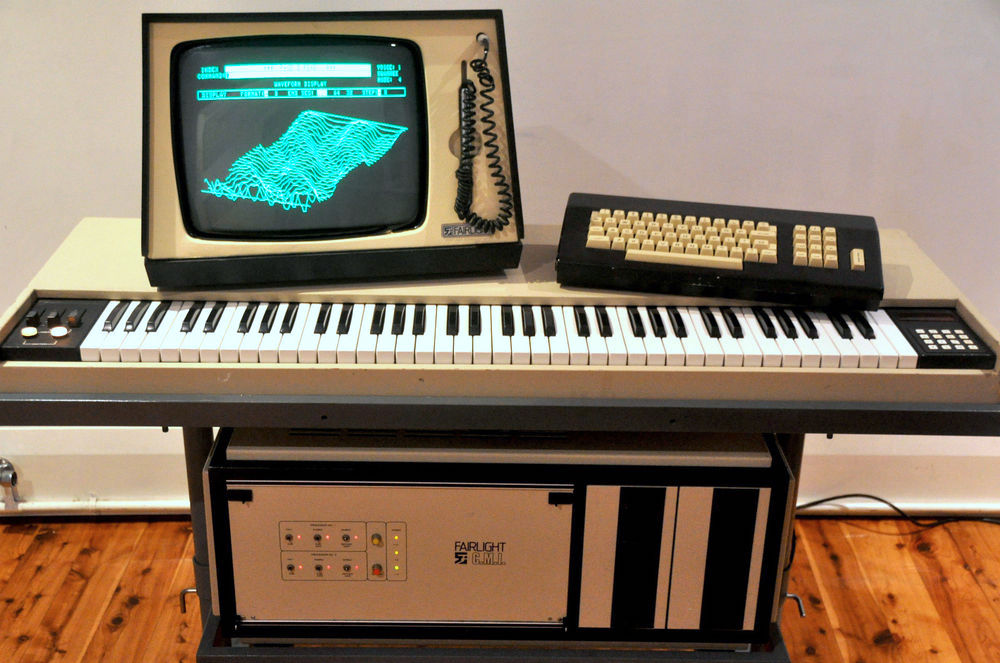
\includegraphics[width=\linewidth]{gfx/05_interfaces/fairlight-CMI.jpg}
		\caption[Le Fairlight CMI]{Le \textit{Fairlight CMI} créé en 1976, un synthétiseur et séquenceur utilisant un écran à stylet. Photographie : Peter Wielk.}
		\label{fig:interface:fairlightCMI}
	\end{minipage}
	\hspace{.02\linewidth}
	\begin{minipage}[t]{0.48\textwidth}
	    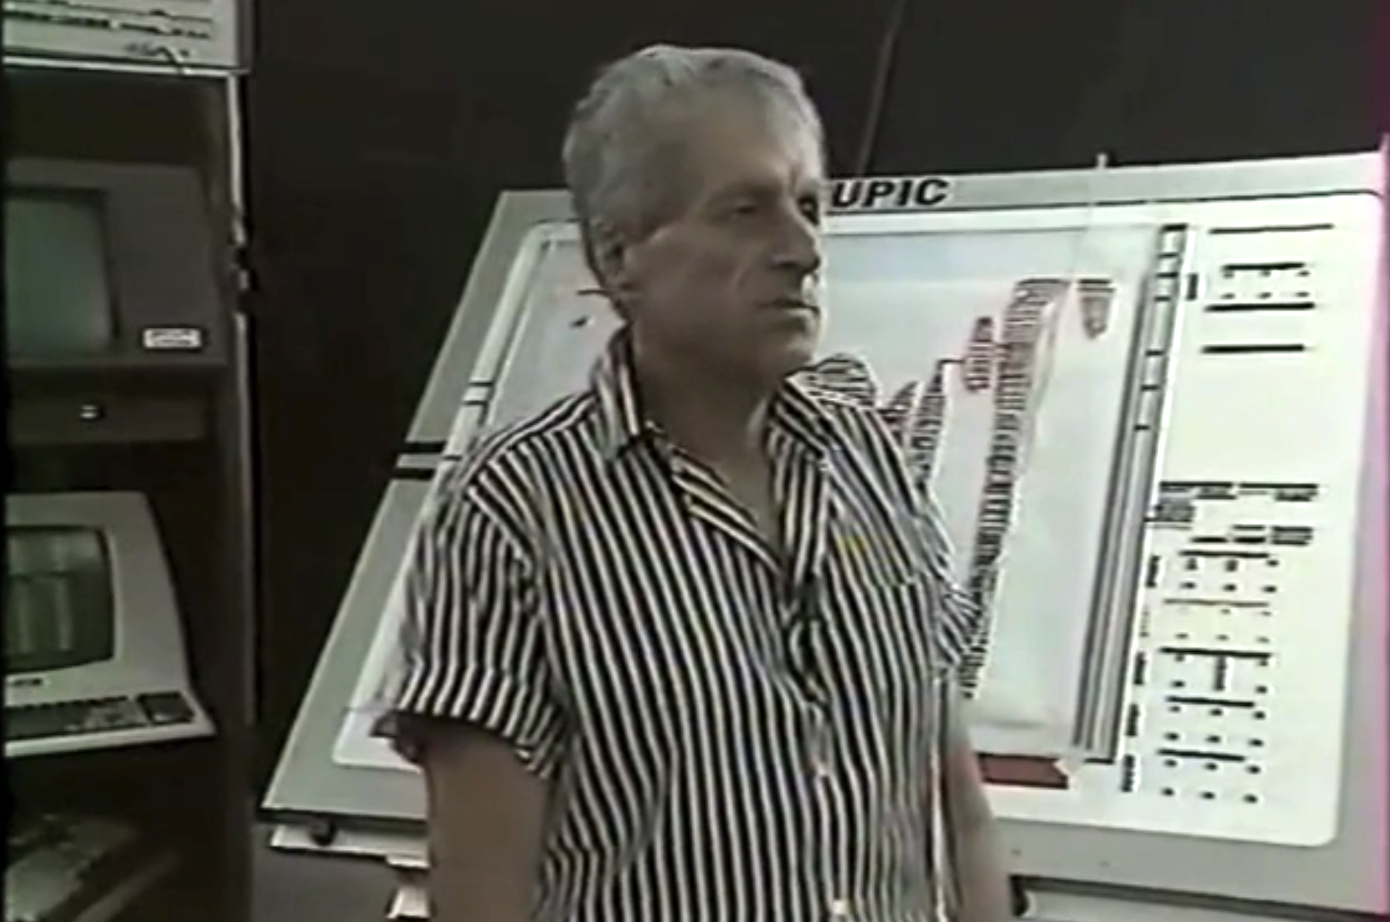
\includegraphics[width=\linewidth]{gfx/05_interfaces/UPIC-Xenakis.png}
		\caption[L'UPIC de Iannis Xenakis]{La station UPIC inventée par Xénakis permet de dessiner des formes graphiques libres, pouvant être lues de différentes manières pour être traduites en son. (Image extraite du documentaire ``Avenir UPIC Xenakis'', centre Xénakis)}
		\label{fig:interface:UPIC}
	\end{minipage}
\end{figure}
%------------ Figure : fairlight CMI et UPIC -----------
\indent À l'origine destinée aux graphistes, les tablettes à stylet ont également été utilisées pour la composition. Le système \textit{UPIC} inventé par Iannis Xénakis (figure \ref{fig:interface:UPIC}) ou le \textit{Fairlight CMI}  (figure \ref{fig:interface:fairlightCMI}) utilisaient tous les deux, dans des directions relativement différentes, une interface basée sur la tablette et le stylet. En dehors de son usage pour la composition, un certain nombre de musiciens, compositeurs et concepteurs de \gls{NIME} l’ont par ailleurs adoptée pour la performance\footnote{Notamment à l'\gls{IRCAM} (voir \cite{wanderley_choice_2000}), au \gls{CNMAT} (voir \cite{zbyszynski_ten_2007}, au \gls{LMA} \cite{couturier_utilisation_2004}, au \gls{LIMSI} \cite{feugere_chorus_2011} puis dans l'équipe \gls{LAM} \cite{xiao_t-voks_2019}, mais on peut également citer Pierre Jodlowski (voir \url{https://youtu.be/pLARXmGwIO4}) ou Jesper Nordin (voir \url{https://gestrument.com/})}. Nicolas d’Alessandro a consacré une partie de son travail de thèse \cite{dalessandro_realtime_2009} à ce sujet, en proposant une étude détaillée des différentes échelles de mouvements dans le geste du dessin et de l'écriture, liées à l'articulation entre doigts, poignet et épaule. J'avais pour ma part utilisé la tablette graphique dans différents projets\footnote{\textit{filigram}, \textit{Media Music rooM}, cf. \url{http://vincentgoudard.com}}, comme un composant parmi d'autres interfaces \gls{MIDI} ou de type joystick, avant de développer plus particulièrement des programmes pour cette interface.\\
\indent Un des inconvénient de la tablette Wacom est que les contours de la surface utile, plus petite que la surface de la tablette\footnote{Cela permet de ne pas ``tomber'' hors de la tablette.}, sont à peine perceptibles, tant visuellement qu'au niveau tactile. Cela s'avère problématique quand on manipule certains processus sonores (et non un pinceau dans PhotoShop, tel que l'usage de la tablette le prévoit), car le regard de l'instrumentiste est souvent déjà occupé par l'attention qu'il/elle aux autres instrumentistes, à une partition, ou un chef d'orchestre. Une première adaptation a donc consisté à rajouter des bandes adhésives permettant de matérialiser cette frontière, visuellement et tactilement (cf. figure \ref{fig:interface:wacom}).\\
%-------------------------- Figure : wacom ---------
\begin{figure}[!htbp]
	\captionsetup{format=plain}%
	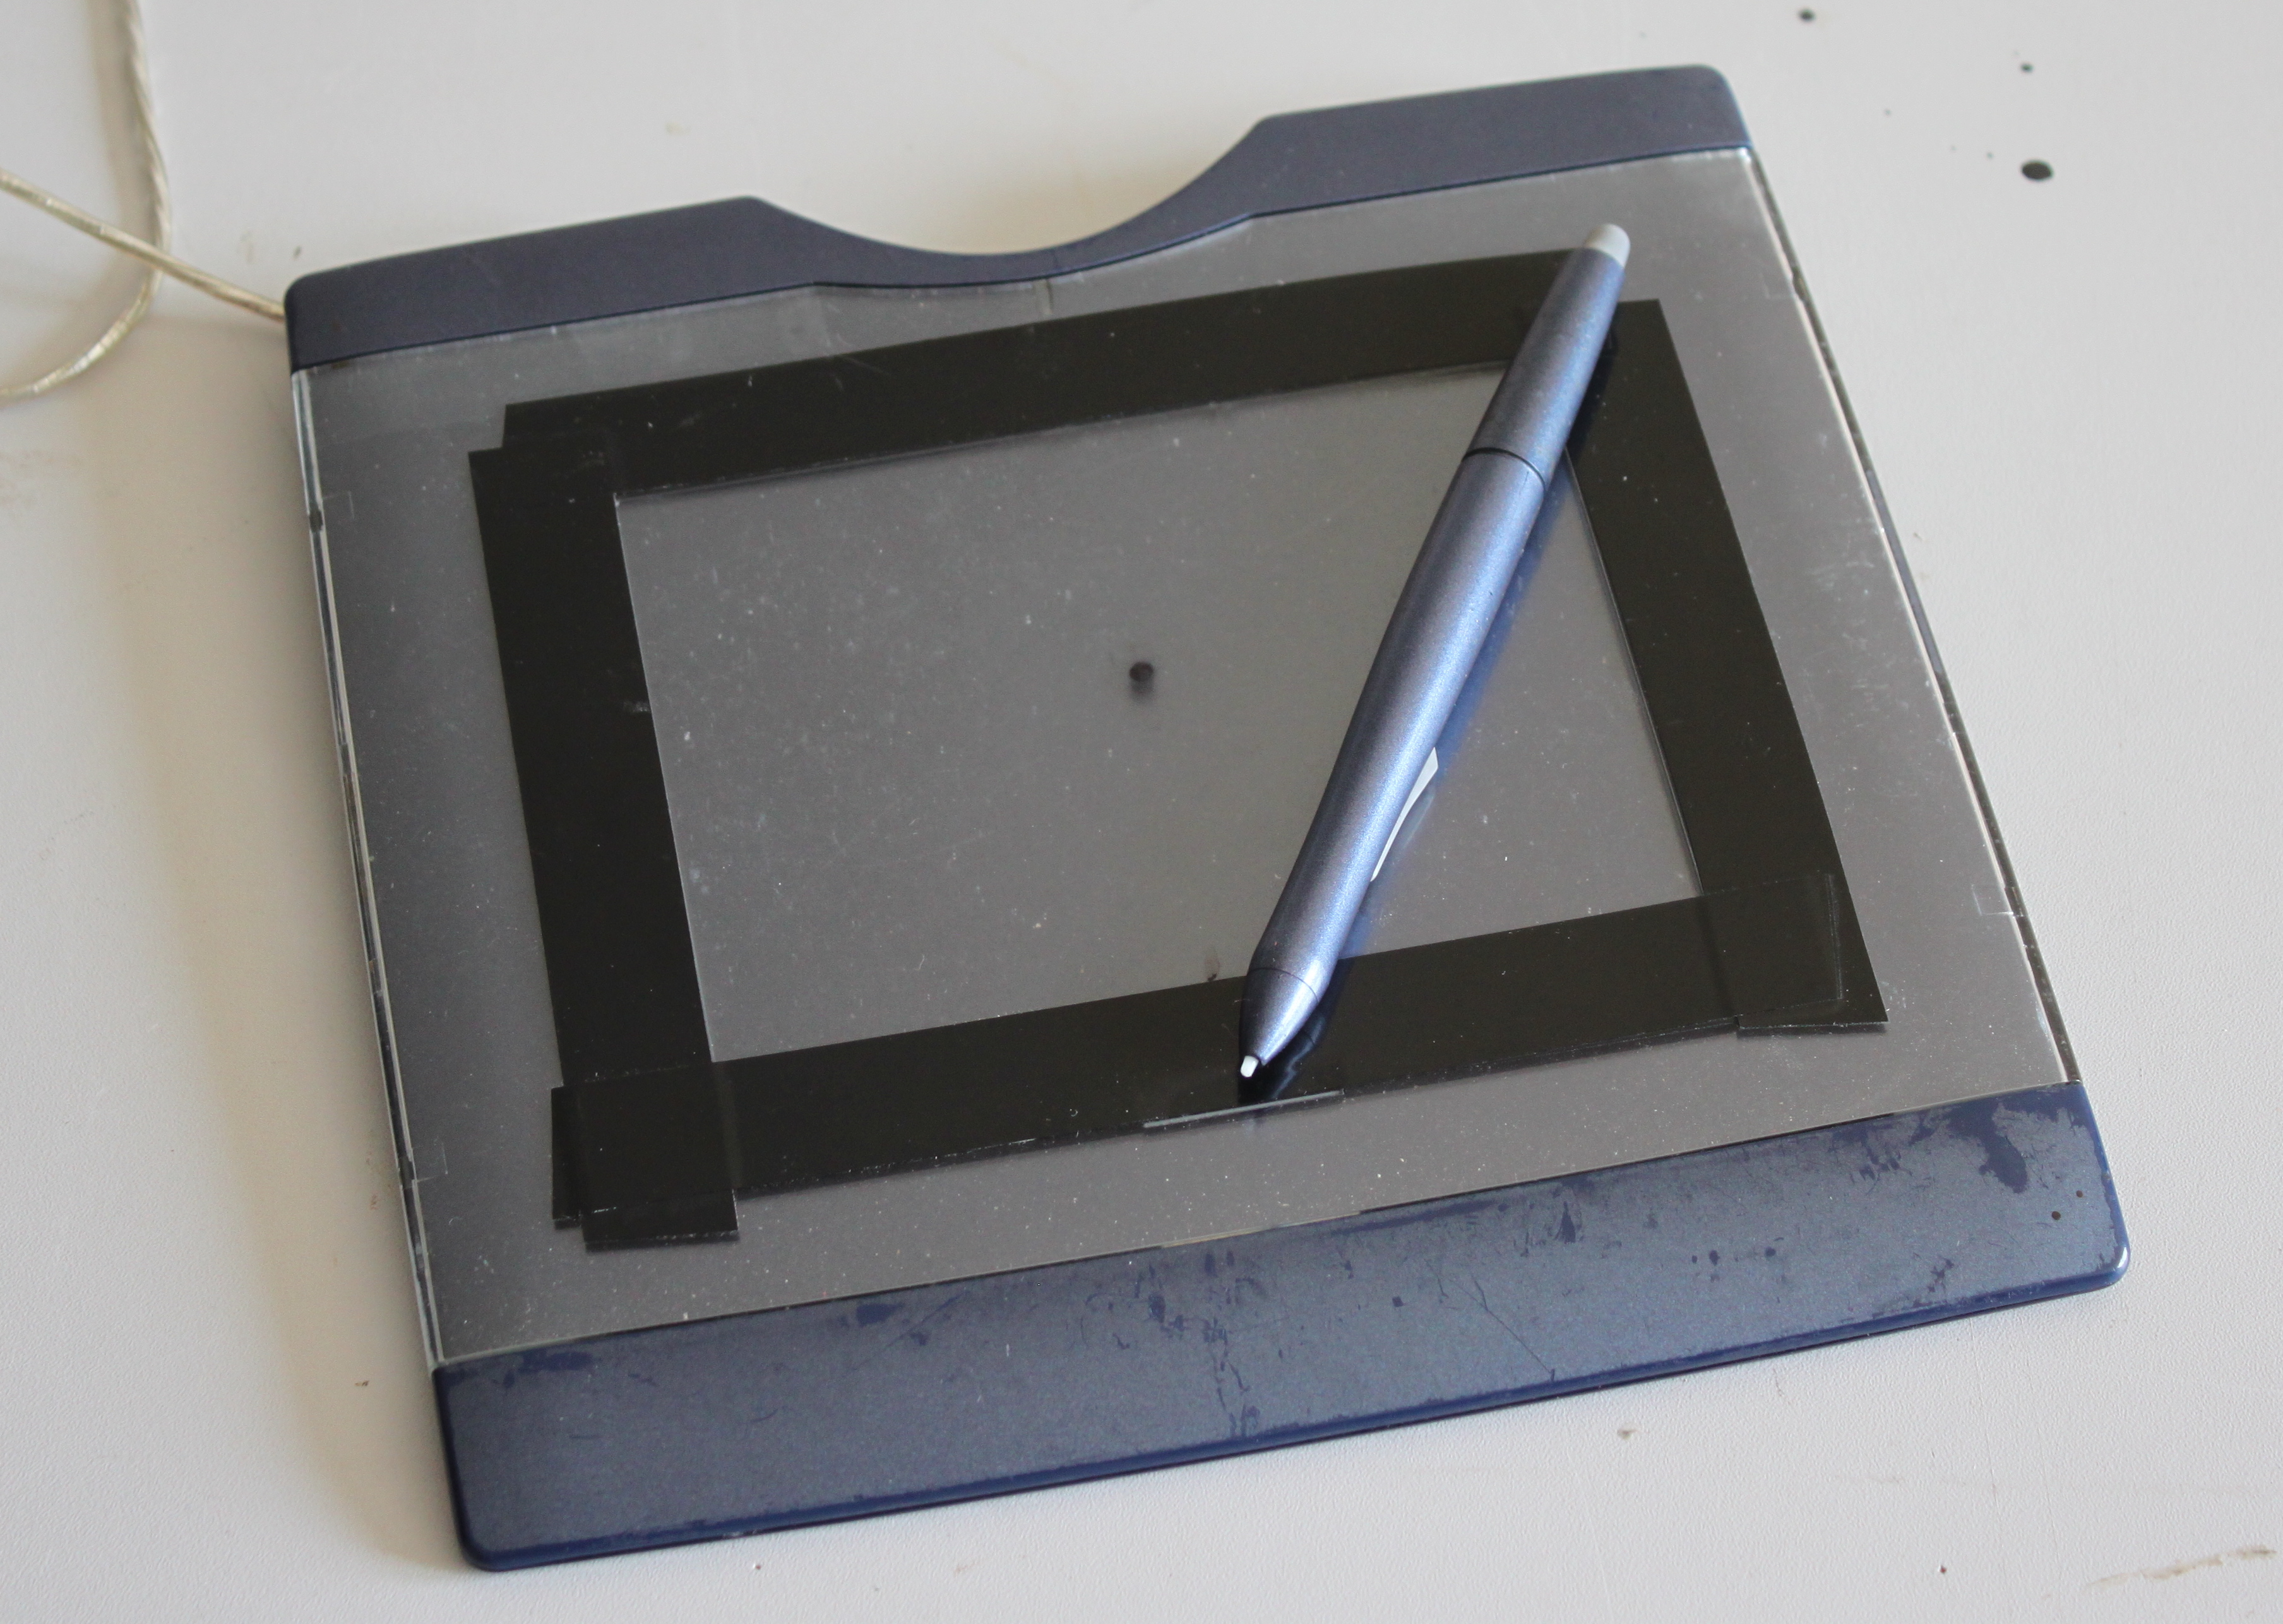
\includegraphics[width=\textwidth]{gfx/05_interfaces/wacom.jpg}
	\caption[Tablette wacom]{Tablette Wacom utilisée à l'origine. Des adhésifs rajoutés en bordure guident la perception haptique, un point central sert de repère visuel.}
	\label{fig:interface:wacom}
\end{figure}
%-------------------------- Figure : wacom ---------
\indent En 2007, dans l'équipe \gls{LAM}, Hugues Genevois avait acquis de nouveaux transducteurs tactiles large bande\footnote{Cette nouvelle génération offrait une bande passante de l'ordre du Hz jusqu'à plusieurs kHz, bien supérieure aux actuateurs linéaires, ainsi qu'une dynamique supérieure à celle des transducteurs piezo. Cette technologie a depuis équipé de nombreux cinémas pour donner au spectateur une expérience plus tactile du son.}. Nous avons fait l'expérience d'en placer un sous une tablette graphique, sur laquelle nous contrôlions la lecture d'un échantillon en se servant du stylet comme d'une tête de lecture virtuelle. La sensation haptique résultant était tout à fait saisissante et donnait l'impression que la surface de la tablette avait un relief physique similaire aux reliefs perçus dans le son : littéralement, l'impression de ``toucher le son''. Ce ``relief'' artificiel est bien entendu éphémère car ces transducteurs ne transmettent pas le continu et leur course est faible\footnote{Ceci les différencie nettement des systèmes de retours haptiques tels que développés, en particulier, à l'\gls{ACROE}}, mais la sensation est tout à fait confondante. J'ai donc utilisé ce système directement sur la tablette graphique, qui était une sorte de prototype du Filigramophone présenté ci-après.

%----------------------------------------------------
\subsection{Le Filigramophone: une tablette augmentée (2013)}
\label{sec:interfaces:phylogenese:filigramophone}

%-------------------------- Figure : filigramophone ----------------------------------
\begin{figure}[!htbp]
	\includegraphics[width=\textwidth]{gfx/filigramophone/filigramophone_overview.jpg}
	\caption{filigramophone - vue d'ensemble, débranchée}
	\label{fig:interface:filigramophone}
\end{figure}
%----------------------------------------------------------------------------------------------------------
\noindent L'expérience décrite précédemment a sucité le développement d'une interface plus intégrée, augmentant la tablette graphique d'une dimension acoustique bi-directionnelle, en captant d'une part le son de la tablette à l'aide de microphones piezo et en diffusant des signaux audio dans la tablette à l'aide de transducteurs tactiles.

\subsubsection{Intégration des microphones piezo}

\noindent En effet, si la tablette graphique est une interface relativement expressive, par la possibilité qu'elle offre de contrôler trois, voire cinq variables continues en même temps\footnote{La position horizontale et verticale, la pression, et sur certains modèle, l'inclinaison du stylet selon les deux axes.}, sa fréquence d'échantillonage reste relativement faible\footnote{Généralement de 100Hz, d'après Wacom, mais l'objet wacom recevant les données de manière asynchrone dans Max ne permet pas la pleine exploitation de cette fréquence.} et la latence importante\footnote{La latence entre le mouvement du stylet et l'arrivée des données est de l'ordre de 50ms, alors qu'elle est de l'ordre de 5ms pour le \gls{MIDI}.}. Le désir de l'augmenter de microphones est ainsi largement lié à cette sensation de distance, qu'on retrouve de manière générale dans la plupart des interfaces de contrôle de type \gls{MIDI} (bien que moindre dans le \gls{MIDI}, cette distance est également sensible).\\
\indent Ali Momeni avait réalisé ce type d'augmentation acoustique, en plaçant un microphone piezo directement sur la tablette\footnote{Développements présentés dans sa thèse \cite{momeni_composing_2005}}. Cette technique lui permet de \iquote{Taper, gratter, frapper avec un anneau métallique ou frotter la tablette} pour obtenir une variété de signaux audio captés par le microphone piezo.\\
\indent Plus récemment, Romain Michon a étudié différentes possibilités d'effectuer des gestes percussifs et de pression sur une tablette \textit{multitouch}\footnote{Voir \cite{michon_nuance_2016}}, et proposé une solution hybride par l'ajout de capteurs \gls{FSR} placés sous un iPad, modulés en amplitude et récupérés via l'entrée audio d'un iPad. L'intérêt de cette solution est de permettre le calcul de la vélocité des gestes percussifs, en plus de l'aftertouch, mais la fusion des informations de pression et de coordonnées X/Y, bien que judicieusement contournée par une triangulation des différents \gls{FSR}, reste problématique comme le remarque son auteur. Par ailleurs, cette solution utilisant des capteurs de pression, sous la surface rigide de l'iPad ne permet pas d'exploiter la variation de hauteur spectrale en fonction du lieu de frappe, la surface de l'iPad étant trop rigide et les \gls{FSR} inadaptés à cette gamme de fréquences.\\
%------------ Figure : filigramophone et xypre piezo -----------
\begin{figure}[!htbp]
	\captionsetup{format=plain}%
	\centering
	\begin{minipage}[t]{0.48\textwidth}
		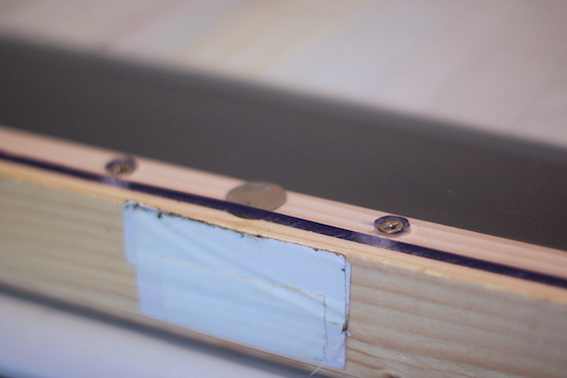
\includegraphics[width=\linewidth]{gfx/05_interfaces/filigramophone-piezo_72dpi.jpg}
		\caption{Transducteur piezo entre la vitre et le chassis sur le Filigramophone}
		\label{fig:interface:filigramophone-piezo}
	\end{minipage}
	\hspace{.02\linewidth}
	\begin{minipage}[t]{0.48\textwidth}
		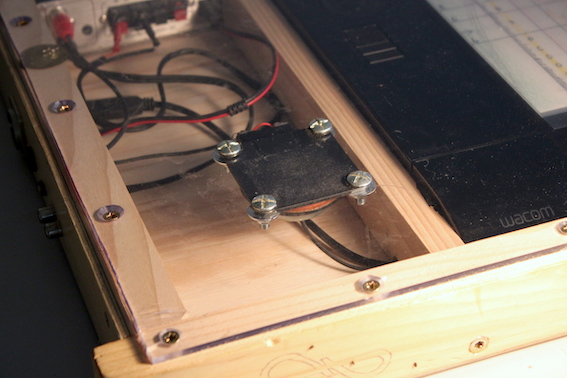
\includegraphics[width=\linewidth]{gfx/05_interfaces/filigramophone_hp_72dpi.jpg}
		\caption{HP tactile sur le Filigramophone}
		\label{fig:interface:filigramophone-hp}
	\end{minipage}
\end{figure}
%------------ Figure : filigramophone et xypre piezo -----------
\indent J'ai pour ma part choisi d'insérer les microphones piezo entre une vitre en \gls{PMMA} et le chassis contenant la tablette graphique (cf. figure \ref{fig:interface:filigramophone-piezo}). Cela permet des gestes percussifs, de frottements ou l'utilisation d'objet mis en mouvement (toupies, dés, diques, etc.) directement sur la surface, tout en conservant --~à travers le \gls{PMMA}~-- l'usage de la tablette qui renvoit les coordonnées horizontale et verticale ainsi que la pression et l'inclinaison du stylet. Ces transducteurs piezo permettent de capter les différents timbres de la surface \gls{PMMA}, qui présente une certaine élasticité (par rapport à la surface rigide de la tablette) en étant fixée uniquement sur ses bords, et dont la hauteur spectrale est plus grave au centre et plus aigüe sur les bords, à la manière d'une peau de tambour. Il est également possible de frapper sur le chassis, ce qui permet d'obtenir encore d'autres nuances de timbre (figure \ref{fig:interface:filigramophone-toupie}). Cette solution évite par ailleurs les bruits ``parasites'' de la structure de la tablette graphique quand on frappe directement dessus. Enfin, l'ajout de la plaque de \gls{PMMA} laisse la possibilité de dessiner, ajouter de l'adhésif, ou graver directement directement sur le \gls{PMMA} (tel que présenté dans la section \ref{todo}), sans déteriorer la tablette. Eventuellement, disposer de différentes plaques de \gls{PMMA} permettrait d'adapter l'interface à différentes configurations, à la manière des ce que permettent les \textit{overlays} sur les interfaces commerciales \textit{Joué} et \textit{SenselMorph}\footnote{\url{https://www.play-joue.com}, \url{https://sensel.com}}, ou à des compositions différentes, telles que les ``\textit{tangible scores}'' d'Enrique Tomás \cite{tomas_tangible_2014}.

%-------------------------- Figure : filigramophone-toupie ----------------------------------
\begin{figure}[!htbp]
	\captionsetup{format=plain}%
	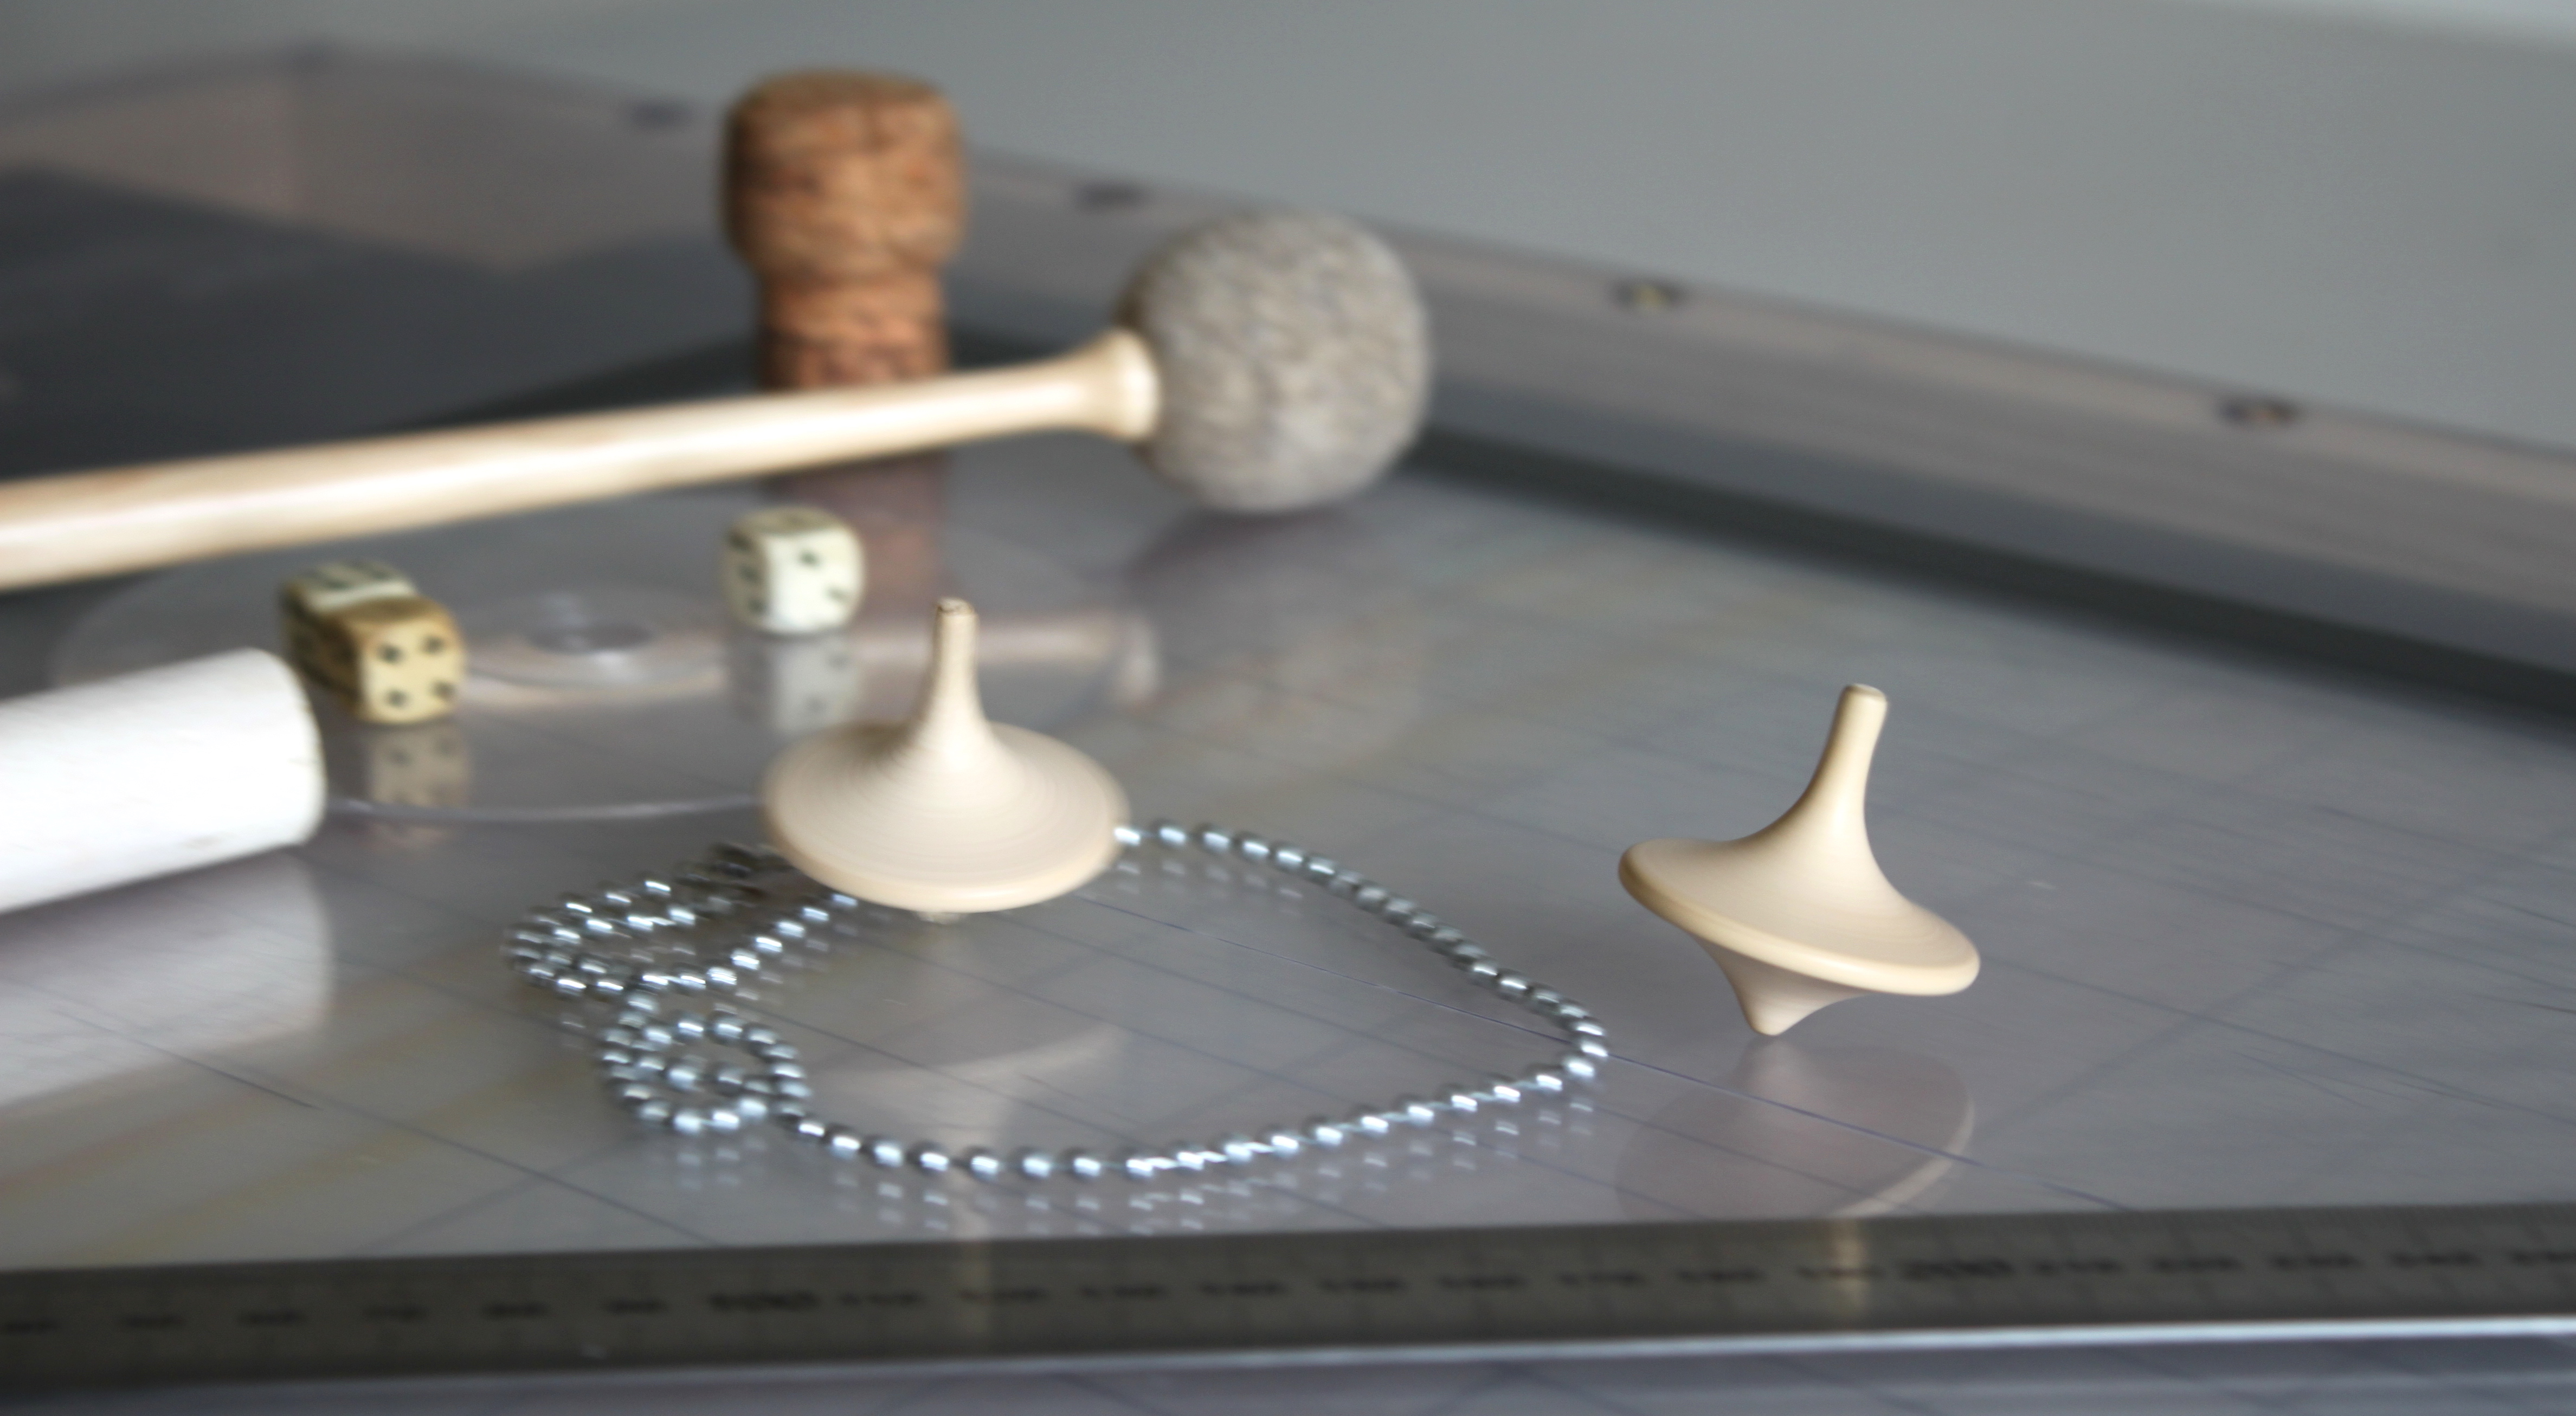
\includegraphics[width=\textwidth]{gfx/05_interfaces/filigramophone-toupie.jpg}
	\caption[Captation du son des mains ou d'objets sur la surface du Filigramophone]{Le microphone piezo laisse la possibilité de capter le son des mains ou d'objets sur la surface du Filigramophone}
	\label{fig:interface:filigramophone-toupie}
\end{figure}
%-------------------------- Figure : filigramophone-toupie ----------------------------------

\subsubsection{Intégration du transducteur tactile}

\noindent Parallèlement, un transducteur a été fixé sur la vitre de \gls{PMMA} (cf. figure \ref{fig:interface:filigramophone-hp}), et positionné empiriquement\footnote{c'est-à-dire, par un balayage des fréquences, envoyé sur le transducteur, en écoutant et en touchant la surface pour y trouver les zones de résonance.} pour favoriser l'excitation des premiers modes de résonance de la plaque de \gls{PMMA} sans être toutefois dans la zone d'interaction de la tablette graphique. Les premiers modes de résonance correspondent en effets aux fréquences les plus basses, et le but était ici d'avoir une vibration aussi forte que possible dans un domaine vibrotactile qui n'empiète pas trop sur le domaine audible.\\
\indent Le transducteur tactile est utilisé à la fois pour le retour vibratoire et la communication d'information, en particulier par frettage virtuel de la surface (cf. infra, section \ref{sec:audio-fretting}). Le retour vibratoire de l'instrument se distingue toutefois de l'envoi pur et simple du signal audio, la perception tactile ne lui étant pas directement liée. Au lieu de cela, un signal sinusoidal à 70Hz, correspondant à une fréquence de résonnance de la vitre de \gls{PMMA}, modulé par l'enveloppe du son final, ainsi que par sa dérivée spectrale, afin de mieux sentir dans les doigts les transitions et les ruptures du son.\\
%(cf. figure TODO : schéma de principe du patch / développement dans une autre partie ?).\\
\indent Le Filigramophone a été joué plusieurs fois en concert, à la fois dans l'ensemble ONE, ainsi que dans la première version de la performance audio-visuelle ``FIB\_R'' avec la plasticienne Gladys Brégeon (cf. figure \ref{fig:interface:filigramophone-Xypre-Triton}). Le dispositif complet était composé du Filigramophone, d'un ordinateur faisant tourner un patch Max pour la synthèse, d'une carte son et haut-parleurs, ainsi que d'une interface \gls{MIDI} Akai MPD24, donnant un accès direct à davantage de paramètres tels que le volume général, le mixage entre différentes synthèses, le rappel de configurations, la sélection d'échelles musicales pour l'accordage, ainsi que divers autres paramètres spécifiques aux algorithmes de synthèse.

%-------------------------- Figure : fibroscopie Triton ----------------------------------
\begin{figure}[!htbp]
	\captionsetup{format=plain}%
	\includegraphics[width=\textwidth]{gfx/05_interfaces/fibroscopie-Triton.jpg}
	\caption[Filigramophone et prototype du Xypre sur scène]{Filigramophone (à droite) et une version prototypique du Xypre v1 (à gauche) sur scène, durant la répétition de FIB\_R en juin 2015, Le Triton, Les Lilas (93).}
	\label{fig:interface:filigramophone-Xypre-Triton}
\end{figure}
%-------------------------- Figure : fibroscopie Triton ----------------------------------


%---------------------------------------------------------------
\subsection{Xypre : écran multitouch augmenté (2015, 2018)}
\label{sec:interfaces:phylogenese:xypre}
%------------ Figure : xypre - plan et vue d'ensemble -----------
\begin{figure}[!htbp]
	\captionsetup{format=plain}%
	\centering
	\begin{minipage}[t]{0.365\textwidth}
		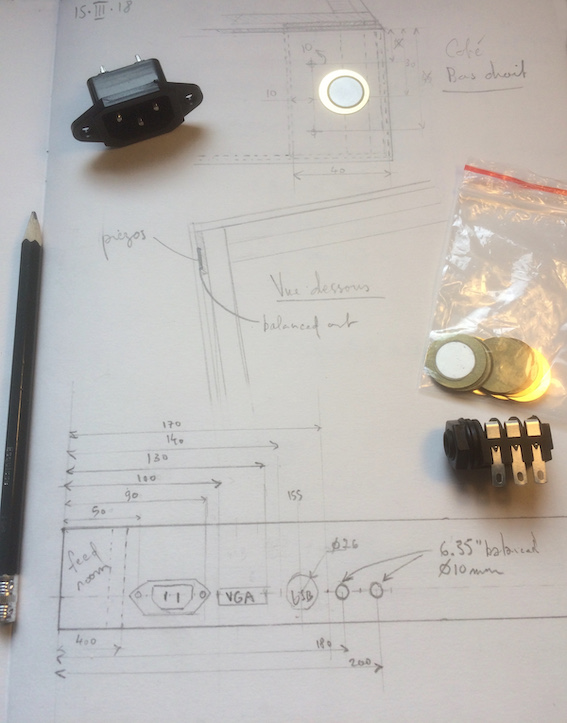
\includegraphics[width=\linewidth]{gfx/05_interfaces/Xypre_plan01_72dpi.jpg}
		\caption{Xypre v2 - plans de conception}
		\label{fig:interface:xypre_plans}
	\end{minipage}
	\hspace{.01\linewidth}
	\begin{minipage}[t]{0.6\textwidth}
	    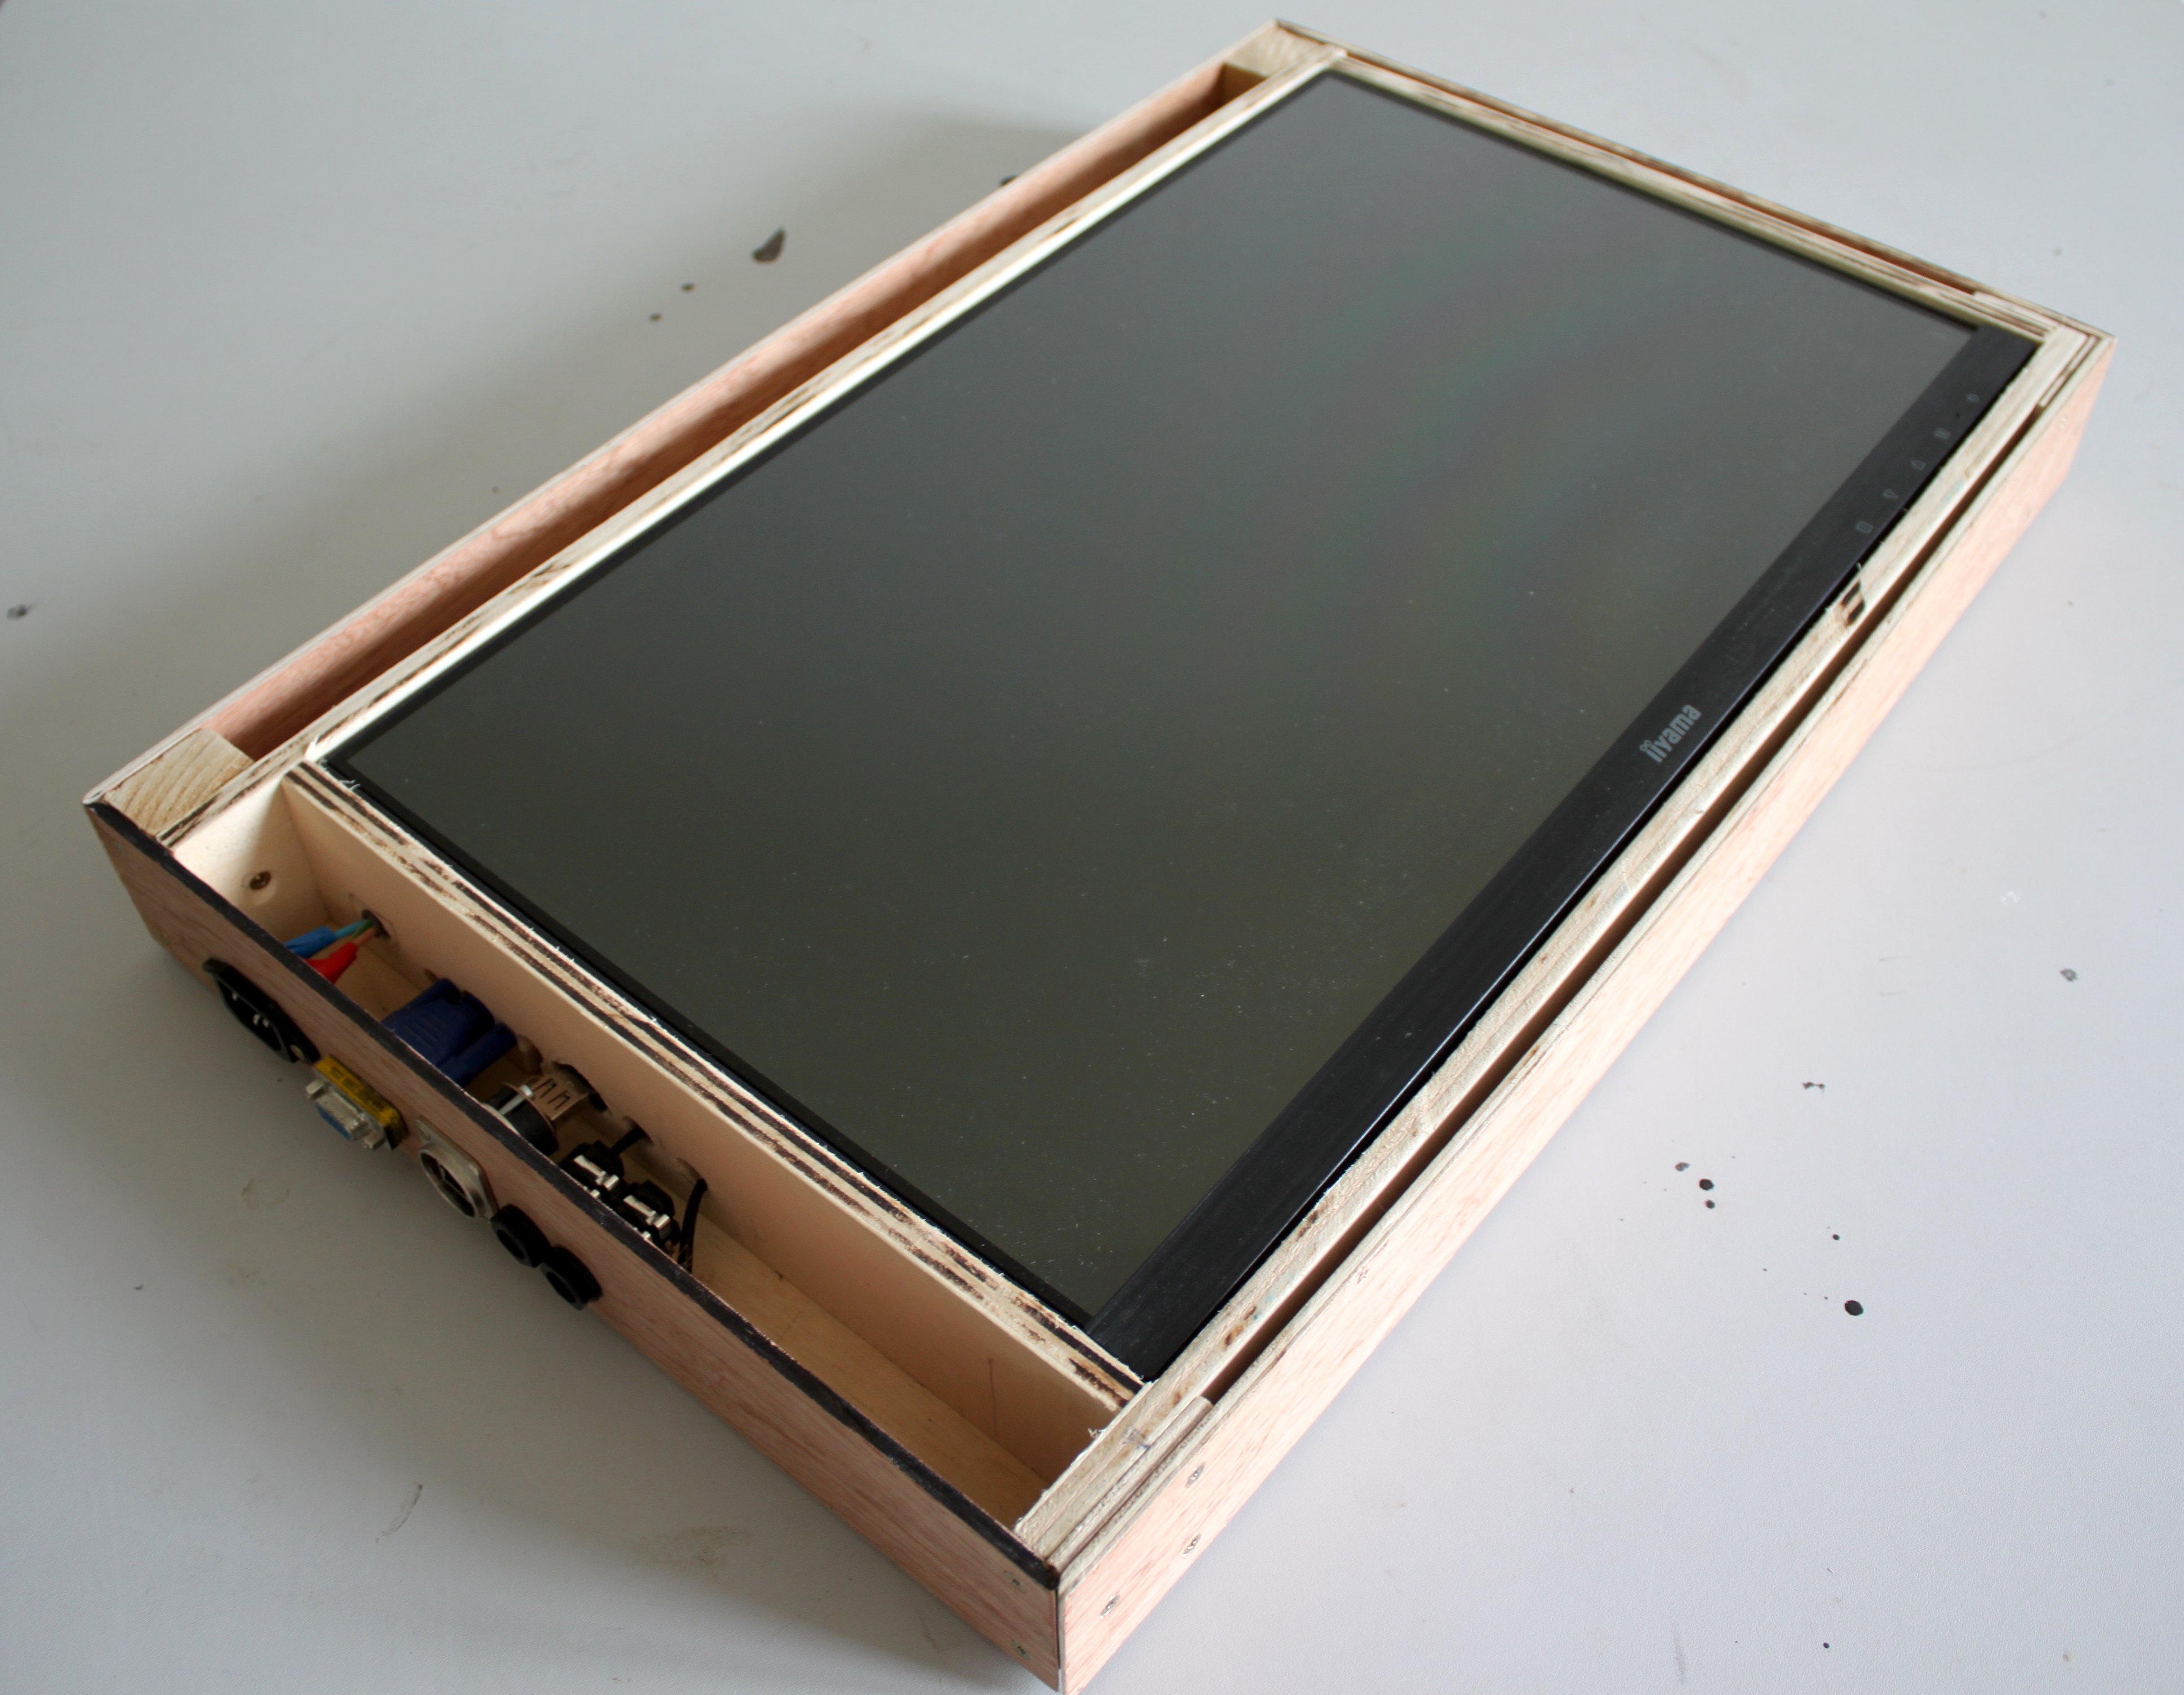
\includegraphics[width=\linewidth]{gfx/05_interfaces/xypre_overview_unplugged.jpg}
		\caption{Xypre - vue d'ensemble, débranchée}
		\label{fig:interface:xypre}
	\end{minipage}
\end{figure}
%------------ Figure : xypre - plan et vue d'ensemble -----------

\noindent L'utilisation du Filigramophone lors de performances musicales a permis de constater plusieurs points d'améliorations possibles, qui ont donné lieu au développement d'une nouvelle interface, nommée Xypre\footnote{Une vidéo montre en accéléré le processus de fabrication de la version 2 du Xypre : \url{https://vimeo.com/358401223}}:
\vspace{-1em}
\begin{itemize}[noitemsep]
	\item La taille de l'interface le rendait intransportable en avion en tant que bagage cabine, et de manière plus courante, peu pratique dans le métro parisien;
	\item Son poids rendait également son transport pénible, malgé une pochette à dessin adaptée\footnote{Un avantage d'un tel format ``tablette'' est qu'il est relativement facile de trouver des sacs d'artiste, habituellement destinés au transport de dessins, dans un grand nombre de formats.}. Notamment le chassis, trop massif, pouvait être allégé;
	\item La nécessité d'une interface complémentaire (le MPD24) augmentait d'autant le temps de montage, de démontage, ainsi que le poids global;
	\item La relative fixité des repères visuels sur le calque de la tablette, qui exigeaient un démontage fastidieux pour être changées, et qui du coup, ne l'étaient pas;
	\item Le jeu polyphonique y était limité, tant par l'unicité du stylet que par l'absence de retour visuel permettant de gérer différentes couches de manière indépendante avec un seul stylet.
\end{itemize}

\noindent Le poids et la taille ont été diminués en utilisant du contreplaqué plus fins pour le chassis et en adoptant un format de valise cabine, offrant une surface équivalente à la surface utile de la tablette graphique utilisée dans le filigramophone, suffisamment large --~quoique juste assez~-- pour permettre des gestes amples impliquant tout le bras.\\
\indent La solution adoptée pour les autres problèmes évoqués a consisté à remplacer la tablette graphique par un écran \textit{multitouch}, toujours augmenté de piezo et transducteurs tactiles, le retour visuel offert par les écrans permettant de virtualiser les contrôleurs physiques utilisés sur l'interface \gls{MIDI} MPD24\footnote{Voir la librairie graphique ``mp.TUI'' développée à cette fin et présentée au chapitre \ref{ch:visual_representation}}.\\
\indent Deux versions du Xypre ont été développées sur ce même principe, mais utilisant deux technologies différentes en ce qui concerne la captation \textit{multitouch} : l'une basée sur la détection par infra-rouge\footnote{Le modèle \textit{G4S-overlay} de la marque PQ-Labs (\url{https://www.pqlabs.com}) permettant théoriquement jusqu'à 32 points de contact simultanément} et l'autre sur une détection capacitive\footnote{Un écran tactile \textit{Iiyama ProLite T2252MSC}, intégrant une technologie ``capacitive projetée'' permettant la détection de dix points de contact simultanément.}. Les deux interfaces communiquant avec Max via le protocole \gls{TUIO}\footnote{A la différence, toutefois, que le G4S envoit directement des données \gls{TUIO} exploitables dans Max, alors que l'écran capactitif davantage destiné à un usage grand public ne les renvoit pas. Un driver payant, développé par la société \textit{Touch-Base Ltd.} est nécessaire pour convertir les données au format \gls{TUIO}.}, peu d'adaptations ont été nécessaires sur le patch Max gérant l'interaction et la synthèse audio. Toutefois, cette différence de technologie a des conséquences sur l'assemblage et sur les modes de jeu possibles. 

\subsubsection{Technologie multitouch et incidence sur le jeu}

\noindent La technologie infra-rouge de l'\textit{overlay G4S} laisse la possibilité de poser des objets sur la surface, qui soient détectés par les capteurs infra-rouge. Cela permet notamment de pouvoir maintenir des processus actifs, par la présence physique d'objets (comme on maintiendrait une note enfoncée sur un orgue à l'aide d'un poids). Un inconvénient de cette technologie est la détection possible des doigts (ou d'objets) entrant dans le plan de détection, situé légèrement au-dessus de la surface de la vitre. Cela requiert par exemple de lever les doigts qui ne jouent pas relativement haut afin qu'il ne soit pas détectés par erreur, et provoque une tension musculaire pénible de la main.Egalement, cette technologie est plus sensible à la poussière qui peut provoquer de fausses détections.\\
\indent A l'inverse de la technologie infra-rouge, le capacitif ne détecte que la présence des doigts et pas celle d'objet quelconques. Il est possible de détecter la présence d'objets dédiés, intégrant un système électrique actif ou passif, stimulant le champ électrostatique de l'écran, ainsi que de reconnaître ces objets à l'aide d'identifiant spatiaux et/ou temporels\footnote{voir notamment \cite{rekimoto_datatiles_2001, yu_tuic_2011}}. Ce type de solution a notamment été utilisé dans l'application \textit{Rotor} de \textit{ReacTable}. Cette solution présente néanmoins l'inconvénient de nécessiter un circuit électronique dédié d'une part, et d'autre part la reconnaissance de l'objet consomme rapidement le nombre de point de contact détectable par l'interface\footnote{Par exemple, la détection de la position et de l'orientation nécessite généralement trois points de contact, ce qui signifie qu'un écran multitouch permettant dix points de contact ne pourra pas détecter plus de trois objets (et un doigt).}, en même temps qu'elle rajoute une latence due à l'analyse du motif déterminé par les points.

\subsubsection{Implantation des microphones piezo et transducteur tactile}
%------------ Figure : xypre piezo et HP -----------
\begin{figure}[!htbp]
	\captionsetup{format=plain}%
	\centering
	\begin{minipage}[t]{0.48\textwidth}
	    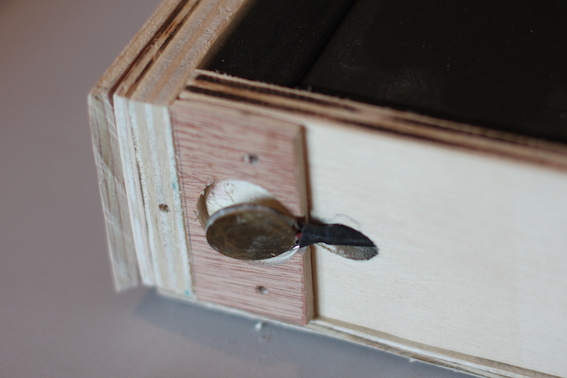
\includegraphics[width=\linewidth]{gfx/05_interfaces/xypre-piezo_72dpi.jpg}
		\caption{Transducteur piezo pseudo-symétrique dans le côté du chassis sur le Xypre v2 (plaque extérieur démontée)}
		\label{fig:interface:xypre_v2-piezo1}
	\end{minipage}
	\hspace{.02\linewidth}
	\begin{minipage}[t]{0.48\textwidth}
	    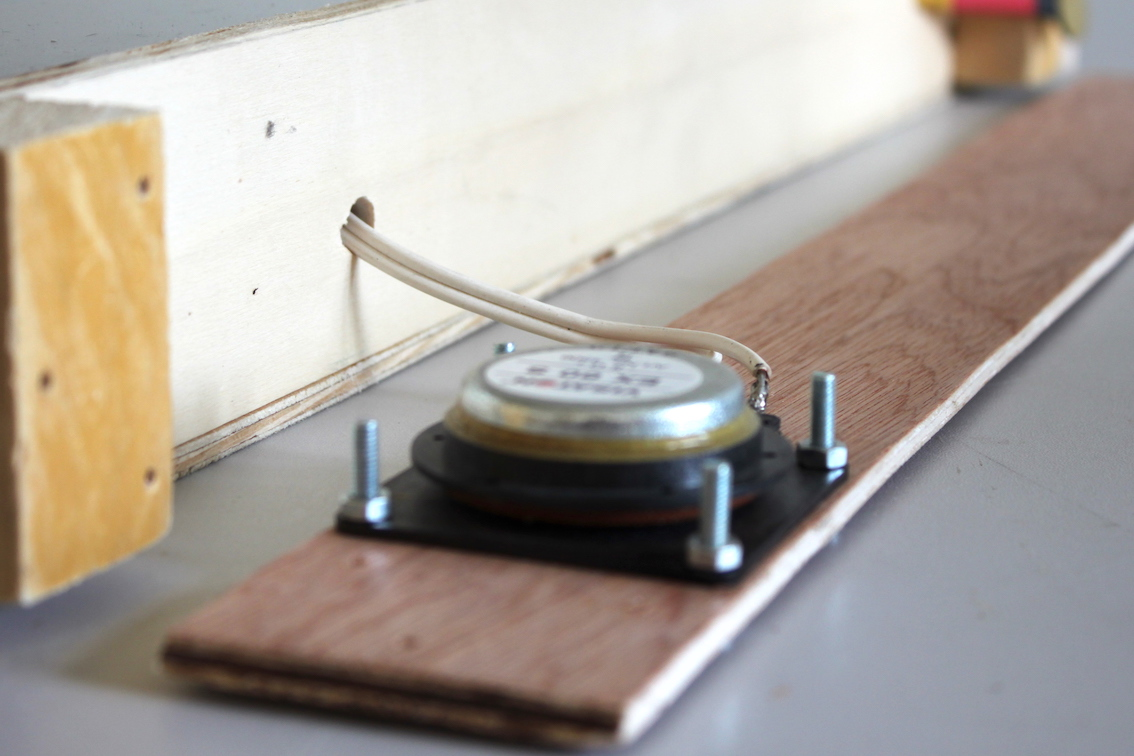
\includegraphics[width=\linewidth]{gfx/05_interfaces/Xypre_HP_144dpi.jpg}
		\caption{HP tactile sur le Xypre}
		\label{fig:interface:xypre_v2-hp}
	\end{minipage}
\end{figure}
%------------ Figure : xypre piezo et HP -----------
%-------------------------- Figure : PQlabs overlay ----------------------------------
\begin{figure}[!htbp]
	\captionsetup{format=plain}%
	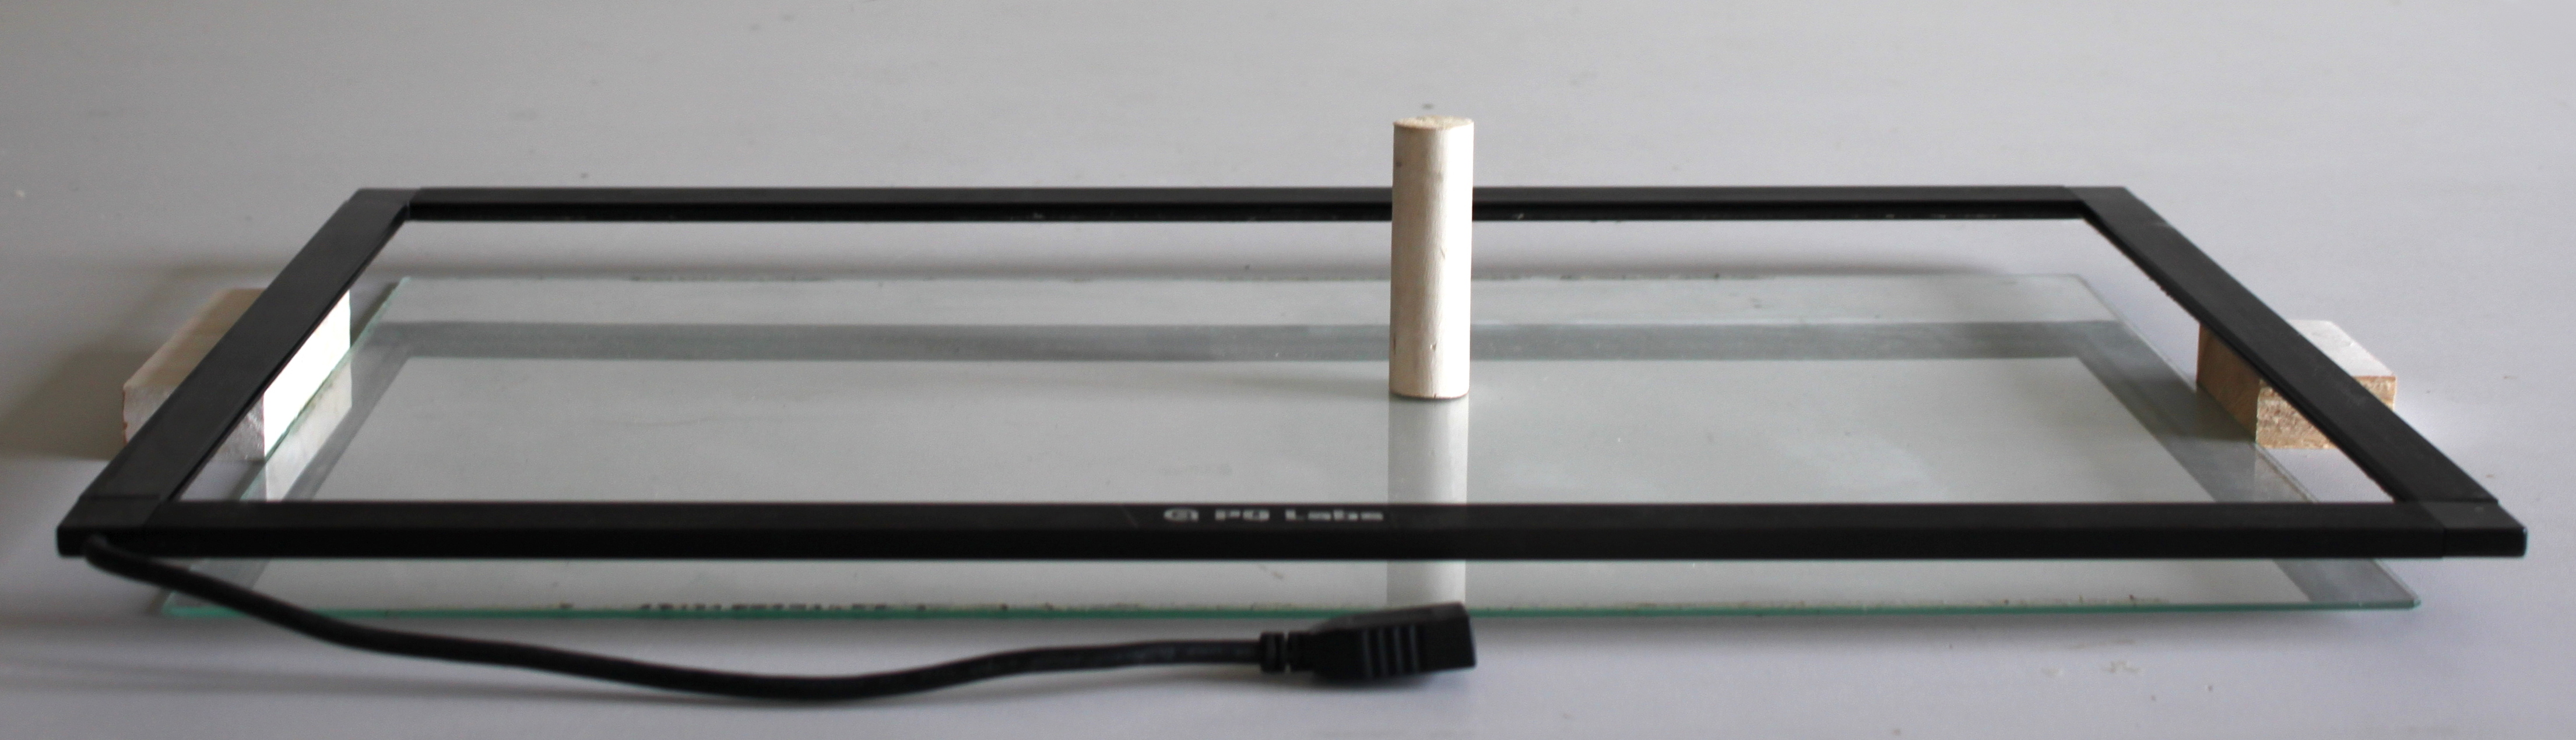
\includegraphics[width=\textwidth]{gfx/05_interfaces/PQlabs-G4overlay.jpg}
	\caption[Cadre multitouch à technologie infra-rouge]{Cadre multitouch à technologie infra-rouge (PQ-Labs). La surface de contact en verre est détachable et la captation d'objets quelconques est possible.}
	\label{fig:interface:PQlabs-G4overlay}
\end{figure}
%-------------------------- Figure : PQlabs overlay ----------------------------------

\indent \textbf{Sur le Xypre v1}, la technologie infra-rouge du cadre de détection du \textit{multitouch} permet d'insérer une vitre en \gls{PMMA} (cf. figure \ref{fig:interface:PQlabs-G4overlay}), pour un fonctionnement similaire à celui développé sur le Filigramophone. L'inconvénient qui résulte des gestes de percussion sur cette vitre est la transmission des vibrations au cadre de détection \textit{multitouch} et les bruits de plastique parasites qu'elles provoquent. Il serait envisageable de supprimer ces bruits en serrant le cadre multitouch entre des mousses, mais cet assemblage plus complexe n'a pas encore été testé.

\indent \textbf{Sur le Xypre v2}, l'écran \textit{multitouch} capacitif ne permettant pas l'ajout d'une vitre \gls{PMMA}, les microphones piezo ont été placées sur le côté du chassis, pré-contraints entre le chassis et une plaque de bois plus fine servant de surface de percussion. Cette plaque fixée sur deux côtés au chassis permet là-encore de récupérer différentes nuances de hauteur spectrale, utilisée pour la synthèse en aval (cf. figure \ref{fig:interface:xypre_v2-piezo1}). La pré-contrainte du piezo est en partie dûe à l'orientation verticale du piezo (qui chuterait, autrement) mais permet également d'utiliser une technique de pseudo-symétrisation du signal du piezo (cf. schéma fonctionnel figure \ref{fig:interface:balancedPiezo} et aperçu figure \ref{fig:interface:xypre_v2-piezo1}), qui s'avère très utile quand les transducteurs piezo sont utilisés à proximité d'un écran, source de perturbations électromagnétiques.\\
%-------------------------- Figure : balanced piezo ----------------------------------
\begin{figure}[!htbp]
	\captionsetup{format=plain}%
	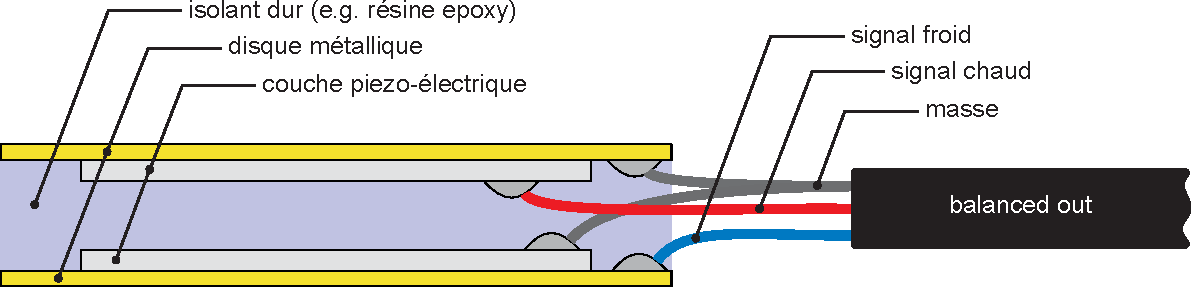
\includegraphics[width=\textwidth]{gfx/05_interfaces/balancedPiezo.pdf}
	\caption{Montage pseudo-symétrique de transducteurs piezo-électriques}
	\label{fig:interface:balancedPiezo}
\end{figure}
%-------------------------- Figure : balanced piezo ----------------------------------
\indent La séparation entre la surface percussive et l'interface \textit{multitouch} de l'écran a conduit à placer le haut-parleur tactile sur une plaque de contreplaqué à l'avant du chassis (cf. figure \ref{fig:interface:xypre_v2-hp}). Il se trouve ainsi relié acoustiquement au transducteur piezo \#2 (cf. figure \ref{fig:interface:xypre_v2-hppiezo}), tandis que l'autre transducteur (figure \ref{fig:interface:xypre_v2-piezo1}) est (relativement) isolé acoustiquement en étant positionné orthogonalement.

%-------------------------- Figure : xypre HP et piezo ----------------------------------
\begin{figure}[!htbp]
	\captionsetup{format=plain}%
	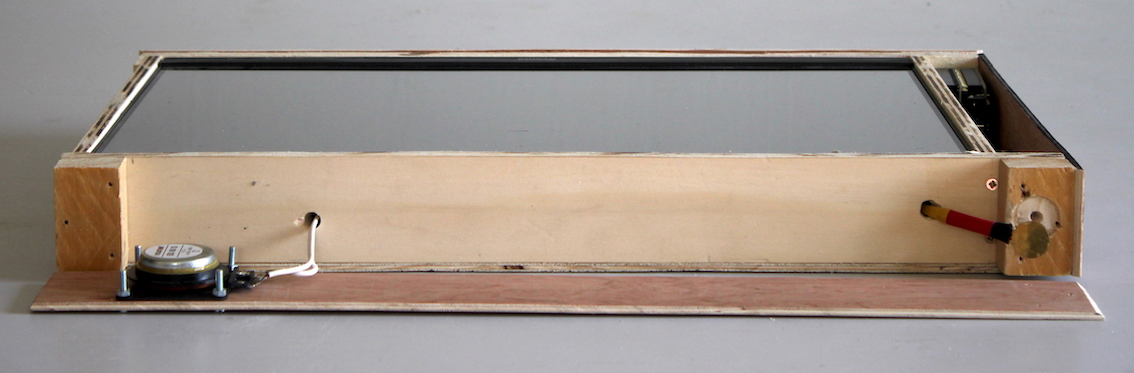
\includegraphics[width=\textwidth]{gfx/05_interfaces/Xypre_FrontPanel_144dpi.jpg}
	\caption{Liaison acoustique entre piezo et haut-parleur tactile sur le Xypre}
	\label{fig:interface:xypre_v2-hppiezo}
\end{figure}
%-------------------------- Figure : xypre HP et piezo ----------------------------------


%-------------------------- Figure : xypre ----------------------------------
\begin{figure}[!htbp]
	\captionsetup{format=plain}%
	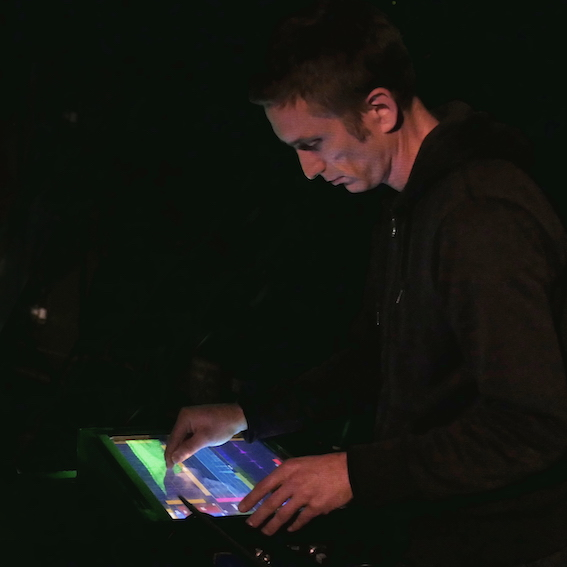
\includegraphics[width=\textwidth]{gfx/05_interfaces/xypre-v1_72dpi.jpg}
	\caption{Xypre v1 inauguré durant une performance avec ONE}
	\label{fig:interface:xyprev1_jeu}
\end{figure}


\subsection{Bilan et perspectives}

\noindent Si les interfaces multitouch conservent une parenté avec les tablettes graphiques, elles offre de nouvelles possibilités en même temps qu'elle impose d'autres contraintes. En particulier, la perte de la pression du stylet comme paramètre expressif est difficile à compenser et à distribuer dans d'autres gestes sans revoir considérablement le design d'interaction en aval. Il est tout de même prévu de rajouter des capteurs de type \gls{FSR} et capteurs de distance, d'une granularité temporelle et d'une expressivité intermédiaire entre celle permise par les microphones et celle permise par l'écran tactile.\\
\indent Une autre direction de développement (en cours), est l'autonomisation progressive de l'interface, en transférant le calcul de la synthèse audio et graphique depuis l'ordinateur sur lequel il tourne maintenant, vers des nano-ordinateurs tels que Raspberry Pi et Bela\footnote{\url{https://raspberrypi.org}, \url{https://bela.io}.}, tout en conservant une extension possible par l'ordinateur.\\
\indent Enfin, au niveau acoustique, l'usage de plaque de bois massive et/ou de métal est envisagé afin d'améliorer la liaison acoustique entre le microphone piezo et le transducteur tactile en façade. Si les premiers tests révelent des interactions intéressantes sur le contrôle du feedback (qu'on espère améliorer en utilisant une carte Bela à très faible latence), le contreplaqué semble un matériau trop épais et absorbant pour que des pressions directe sur la plaque interagissent efficacement avec la boucle de \textit{feedback}.

%%%%%%%%%%%%%%%%%%%%%%%%%%%%%%%%%%%%%%%%%

\section{Conclusion}
\label{sec:interfaces:conclusion}

\noindent L'importance croissante du découplage énergétique entre les gestes de l'instrumentiste et la production du son, depuis l'orgue, qui en donne les premiers signes manifestes, jusqu'aux \glspl{DMI}, qui finissent d'achever cette scission, a entraîné une séparation physique de l'interface de jeu. En effet, comme l'énonce Thor Magnusson, \iquote{on peut dire que l'instrument électronique ou numérique \textbf{a} une interface, tandis que l'instrument acoustique \textbf{est} l'interface\footnote{``We can state that the electronic or digital instrument \textit{has} an interface, whereas the acoustic instrument \textit{is} the interface.'' \cite{magnusson_sonic_2019} (italiques de l'auteur)}.}.\\
\indent Les \glspl{DMI} ne sont plus nécessairement des ``objets que l'on touche''\footnote{Pour les instruments acoustiques, ce rapport au toucher se lit clairement dans le terme italien \textit{Toccata}, ``Œuvres à toucher'', ou l'espagnol \textit{tocar musica}.}, dans la mesure où les capteurs permettent à la fois d'étendre l'interaction à un espace externe à l'objet qui capte le mouvement, ou interne au corps même de l'instrumentiste. L'agencement des capteurs sur l'interface de jeu définit la topologie spatiale de l'interaction gestuelle possible. Il est cependant difficile, comme nous l'avons ici objecté, d'établir un lien univoque entre les types de capteurs utilisés et les fonctions musicales que l'on cherche à moduler, tant il est possible d'interpréter et de re-segmenter les données issues des capteurs de différentes manières, à l'aide d'algorithmes de \textit{mapping}.\\
\indent Cette séparation permet de repenser de manière beaucoup plus ouverte la distribution spatiale de l'instrument, son ergonomie gestuelle, ainsi que la temporalité des relations gestuelle-sonore, dans un champ de possibles qui pourrait s'apparenter à une vertigineuse page blanche. Le design de cette interface est toutefois polarisé par un certain nombre de facteurs matériels (poids, encombrement, matériaux physique, temps de montage, portabilité, etc.) qui conditionnent l'usage effectif des \glspl{DMI} pour la performance musicale.\\
\indent Les interviews menées auprès de musiciens et l'étude des pratiques musicales impliquant des \glspl{DMI} indiquent ici un éventail très large de configurations d'interface, de l'objet physique massif à sa disparition la plus complète, de sa référence à l'instrument traditionnel (dans les instruments augmentés)
à sa prise de distance la plus manifeste (The Sponge), de sa fonctionnalité la plus technique (e.g. les interfaces de contrôle à potentiomètres) à sa présence essentiellement scénographique et poétique (e.g. Lungta).\\
\indent Leur diversité les rend ainsi difficiles à classer en raison des multiples héritages et desseins dont s'inspire leur design, mais le design de l'agencement instrumental semble inséparable d'une considération globale de l'interaction musicale et du projet artistique qu'il sert. Avant même que le musicien ne soit présent pour interagir avec son instrument, la présence physique de l'instrument (ou son absence) se manifeste par dans l'interface de jeu. Sa configuration évoque à la fois les postures corporelles et les gestes qu'appelle cette interface, mais possède également une force propre d'évocation poétique, souvent liée à des référence extra-instrumentales.\\
\indent Les \glspl{DMI}, à la différence des instruments acoustiques, ne sont jamais intégralement construit par une seule et même personne, car les capteurs et processeurs qui les composent sont issus d'une fabrication industrielle qui les rendent dépendants d'une logique de production externe au luthier. Leur fabrication se caractérise ainsi par le fait d'être toujours, fondamentalement, un détournement de matériaux déjà complexes, et rarement conçus à des fins musicales. La description de la conception du filigramophone et du Xypre ont mis en évidence ces aspects, à travers les adaptations apportées en fonctions des caractéristiques techniques de leurs différents composants. Le mapping, au moyens d'algorithmes de transformation et de synthèse, vient encore ajouter à ce détournement, en redéfinissant toutes les relations possibles ou attendues. C'est cette interaction algorithmique que nous allons étudier au prochain chapitre.



%Cette inadéquation des capteurs à l'usage musical possède peut-être une raison plus profonde. Les \glspl{DMI}, à la différence des instruments acoustiques, ne sont jamais intégralement construit par une seule et même personne, car les capteurs et processeurs qui les composent sont issus d'une fabrication industrielle qui les rendent dépendants d'une logique de production externe au luthier. Leur fabrication se caractérise ainsi par le fait d'être toujours, fondamentalement, un détournement de matériaux déjà complexes.


% Les interfaces hardware sont des objets auxquels on s'attache, plus que le virtuel (cf. Dumeaux, Dallio). Rapport sensuel.

% Compromis entre modularité et intégration ergonomique.

% Possibilités offertes par le DIY avec les nouvelles cartes barebone (Ino, raspi, bela, etc.)

% La question de l'acoustique, de l'haptique, de l'électronique et du numérique sont interdépendantes.



% La présentation des différentes version du Filigramophone met en évidence les contraintes imposées par les différents types de capteurs, dont une variation.

%\section*{extra material}

% \iquote{Though there is a huge range of performer decision, history, and knowledge that will determine their exact method of playing (as established by Jorda [12]), the physical design of the DMI impacts this gesture repertoire by presenting certain affordances.} \cite{bin_hands_2017}

% \vspace{-1em}
% \begin{itemize}[noitemsep]
% \item Faire évoluer une interface en la raffinant (De Laubier, VG).
% \item Faire évoluer une interface en rajoutant des choses (Patricia Dallio)
% \item Faire évoluer en supprimant des choses (Dumaux)
% \item Partir de l'objet (Patrick Saint Denis)
% \end{itemize}


% Thor Magnusson : \iquote{On peut dire que l'instrument électronique ou numérique \textit{a} une interface, tandis que l'instrument acoustique \textit{est} l'interface.}\footnote{``We can state that the electronic or digital instrument \textit{has} an interface, whereas the acoustic instrument \textit{is} the interface.''\cite{magnusson_sonic_2019}}
